%
% coif2.tex -- coiflet wavelet 2
%
% (c) 2019 Prof Dr Andreas Müller, Hochschule Rapperswil
%
\documentclass[tikz]{standalone}
\usepackage{amsmath}
\usepackage{times}
\usepackage{txfonts}
\usepackage{pgfplots}
\usepackage{csvsimple}
\usetikzlibrary{arrows,intersections,math}
\begin{document}
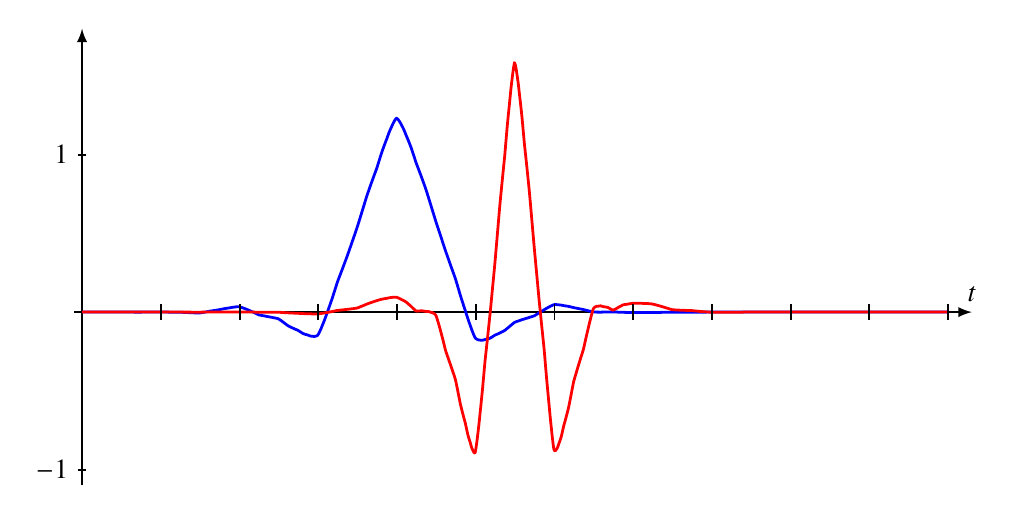
\begin{tikzpicture}[>=latex,yscale=2,xscale=1]

\draw[->,line width=0.7pt] (-0.1,0)--(11.3,0) coordinate[label={$t$}];
\draw[->,line width=0.7pt] (0,-1.1)--(0,1.8);

\draw[line width=1pt,color=blue] (0.00000, 0.00000)
(0.00195, -0.00000)
--(0.00391, -0.00000)
--(0.00586, 0.00000)
--(0.00781, 0.00000)
--(0.00977, -0.00000)
--(0.01172, -0.00000)
--(0.01367, -0.00000)
--(0.01562, -0.00000)
--(0.01758, 0.00000)
--(0.01953, 0.00000)
--(0.02148, 0.00000)
--(0.02344, 0.00000)
--(0.02539, 0.00000)
--(0.02734, -0.00000)
--(0.02930, -0.00000)
--(0.03125, -0.00000)
--(0.03320, -0.00000)
--(0.03516, -0.00000)
--(0.03711, -0.00000)
--(0.03906, -0.00000)
--(0.04102, -0.00000)
--(0.04297, 0.00000)
--(0.04492, 0.00000)
--(0.04688, 0.00000)
--(0.04883, 0.00000)
--(0.05078, 0.00000)
--(0.05273, 0.00000)
--(0.05469, 0.00000)
--(0.05664, 0.00000)
--(0.05859, 0.00000)
--(0.06055, -0.00000)
--(0.06250, -0.00000)
--(0.06445, -0.00000)
--(0.06641, -0.00000)
--(0.06836, -0.00000)
--(0.07031, -0.00000)
--(0.07227, -0.00000)
--(0.07422, -0.00000)
--(0.07617, -0.00000)
--(0.07812, -0.00000)
--(0.08008, -0.00000)
--(0.08203, -0.00000)
--(0.08398, -0.00000)
--(0.08594, -0.00000)
--(0.08789, -0.00000)
--(0.08984, -0.00000)
--(0.09180, 0.00000)
--(0.09375, 0.00000)
--(0.09570, 0.00000)
--(0.09766, 0.00000)
--(0.09961, 0.00000)
--(0.10156, 0.00000)
--(0.10352, 0.00000)
--(0.10547, 0.00000)
--(0.10742, 0.00000)
--(0.10938, 0.00000)
--(0.11133, 0.00000)
--(0.11328, 0.00000)
--(0.11523, 0.00000)
--(0.11719, 0.00000)
--(0.11914, 0.00000)
--(0.12109, 0.00000)
--(0.12305, 0.00000)
--(0.12500, 0.00000)
--(0.12695, 0.00000)
--(0.12891, -0.00000)
--(0.13086, -0.00000)
--(0.13281, -0.00000)
--(0.13477, -0.00000)
--(0.13672, -0.00000)
--(0.13867, -0.00000)
--(0.14062, -0.00000)
--(0.14258, -0.00000)
--(0.14453, -0.00000)
--(0.14648, -0.00000)
--(0.14844, -0.00000)
--(0.15039, -0.00000)
--(0.15234, -0.00000)
--(0.15430, -0.00000)
--(0.15625, -0.00000)
--(0.15820, -0.00000)
--(0.16016, -0.00000)
--(0.16211, -0.00000)
--(0.16406, -0.00000)
--(0.16602, -0.00000)
--(0.16797, -0.00000)
--(0.16992, -0.00000)
--(0.17188, -0.00000)
--(0.17383, -0.00000)
--(0.17578, -0.00000)
--(0.17773, -0.00000)
--(0.17969, -0.00000)
--(0.18164, -0.00000)
--(0.18359, -0.00000)
--(0.18555, -0.00000)
--(0.18750, -0.00000)
--(0.18945, 0.00000)
--(0.19141, 0.00000)
--(0.19336, 0.00000)
--(0.19531, 0.00000)
--(0.19727, 0.00000)
--(0.19922, 0.00000)
--(0.20117, 0.00000)
--(0.20312, 0.00000)
--(0.20508, 0.00000)
--(0.20703, 0.00000)
--(0.20898, 0.00000)
--(0.21094, 0.00000)
--(0.21289, 0.00000)
--(0.21484, 0.00000)
--(0.21680, 0.00000)
--(0.21875, 0.00000)
--(0.22070, 0.00000)
--(0.22266, 0.00000)
--(0.22461, 0.00000)
--(0.22656, 0.00000)
--(0.22852, 0.00000)
--(0.23047, 0.00000)
--(0.23242, 0.00000)
--(0.23438, 0.00000)
--(0.23633, 0.00000)
--(0.23828, 0.00000)
--(0.24023, 0.00000)
--(0.24219, 0.00000)
--(0.24414, 0.00000)
--(0.24609, 0.00000)
--(0.24805, 0.00000)
--(0.25000, 0.00000)
--(0.25195, 0.00000)
--(0.25391, 0.00000)
--(0.25586, 0.00000)
--(0.25781, 0.00000)
--(0.25977, 0.00000)
--(0.26172, 0.00000)
--(0.26367, 0.00000)
--(0.26562, -0.00000)
--(0.26758, -0.00000)
--(0.26953, -0.00000)
--(0.27148, -0.00000)
--(0.27344, -0.00000)
--(0.27539, -0.00000)
--(0.27734, -0.00000)
--(0.27930, -0.00000)
--(0.28125, -0.00000)
--(0.28320, -0.00000)
--(0.28516, -0.00000)
--(0.28711, -0.00000)
--(0.28906, -0.00000)
--(0.29102, -0.00000)
--(0.29297, -0.00000)
--(0.29492, -0.00000)
--(0.29688, -0.00000)
--(0.29883, -0.00000)
--(0.30078, -0.00000)
--(0.30273, -0.00000)
--(0.30469, -0.00000)
--(0.30664, -0.00000)
--(0.30859, -0.00000)
--(0.31055, -0.00000)
--(0.31250, -0.00000)
--(0.31445, -0.00000)
--(0.31641, -0.00000)
--(0.31836, -0.00000)
--(0.32031, -0.00000)
--(0.32227, -0.00000)
--(0.32422, -0.00000)
--(0.32617, -0.00000)
--(0.32812, -0.00000)
--(0.33008, -0.00000)
--(0.33203, -0.00000)
--(0.33398, -0.00000)
--(0.33594, -0.00000)
--(0.33789, -0.00000)
--(0.33984, -0.00000)
--(0.34180, -0.00000)
--(0.34375, -0.00000)
--(0.34570, -0.00000)
--(0.34766, -0.00000)
--(0.34961, -0.00000)
--(0.35156, -0.00000)
--(0.35352, -0.00000)
--(0.35547, -0.00000)
--(0.35742, -0.00000)
--(0.35938, -0.00000)
--(0.36133, -0.00000)
--(0.36328, -0.00000)
--(0.36523, -0.00000)
--(0.36719, -0.00000)
--(0.36914, -0.00000)
--(0.37109, -0.00000)
--(0.37305, -0.00000)
--(0.37500, -0.00000)
--(0.37695, -0.00000)
--(0.37891, -0.00000)
--(0.38086, -0.00000)
--(0.38281, -0.00000)
--(0.38477, 0.00000)
--(0.38672, 0.00000)
--(0.38867, 0.00000)
--(0.39062, 0.00000)
--(0.39258, 0.00000)
--(0.39453, 0.00000)
--(0.39648, 0.00000)
--(0.39844, 0.00000)
--(0.40039, 0.00000)
--(0.40234, 0.00000)
--(0.40430, 0.00000)
--(0.40625, 0.00000)
--(0.40820, 0.00000)
--(0.41016, 0.00000)
--(0.41211, 0.00001)
--(0.41406, 0.00001)
--(0.41602, 0.00001)
--(0.41797, 0.00001)
--(0.41992, 0.00001)
--(0.42188, 0.00001)
--(0.42383, 0.00001)
--(0.42578, 0.00001)
--(0.42773, 0.00001)
--(0.42969, 0.00001)
--(0.43164, 0.00001)
--(0.43359, 0.00001)
--(0.43555, 0.00001)
--(0.43750, 0.00001)
--(0.43945, 0.00001)
--(0.44141, 0.00001)
--(0.44336, 0.00001)
--(0.44531, 0.00001)
--(0.44727, 0.00001)
--(0.44922, 0.00001)
--(0.45117, 0.00001)
--(0.45312, 0.00001)
--(0.45508, 0.00001)
--(0.45703, 0.00001)
--(0.45898, 0.00001)
--(0.46094, 0.00001)
--(0.46289, 0.00001)
--(0.46484, 0.00001)
--(0.46680, 0.00001)
--(0.46875, 0.00002)
--(0.47070, 0.00002)
--(0.47266, 0.00002)
--(0.47461, 0.00002)
--(0.47656, 0.00002)
--(0.47852, 0.00002)
--(0.48047, 0.00002)
--(0.48242, 0.00002)
--(0.48438, 0.00002)
--(0.48633, 0.00002)
--(0.48828, 0.00002)
--(0.49023, 0.00002)
--(0.49219, 0.00002)
--(0.49414, 0.00002)
--(0.49609, 0.00002)
--(0.49805, 0.00002)
--(0.50000, 0.00002)
--(0.50195, 0.00001)
--(0.50391, 0.00001)
--(0.50586, 0.00001)
--(0.50781, 0.00001)
--(0.50977, 0.00001)
--(0.51172, 0.00001)
--(0.51367, 0.00001)
--(0.51562, 0.00001)
--(0.51758, 0.00001)
--(0.51953, 0.00001)
--(0.52148, 0.00001)
--(0.52344, 0.00001)
--(0.52539, 0.00001)
--(0.52734, 0.00001)
--(0.52930, 0.00000)
--(0.53125, 0.00000)
--(0.53320, 0.00000)
--(0.53516, 0.00000)
--(0.53711, 0.00000)
--(0.53906, -0.00000)
--(0.54102, -0.00000)
--(0.54297, -0.00000)
--(0.54492, -0.00000)
--(0.54688, -0.00000)
--(0.54883, -0.00001)
--(0.55078, -0.00001)
--(0.55273, -0.00001)
--(0.55469, -0.00001)
--(0.55664, -0.00001)
--(0.55859, -0.00001)
--(0.56055, -0.00001)
--(0.56250, -0.00001)
--(0.56445, -0.00001)
--(0.56641, -0.00001)
--(0.56836, -0.00001)
--(0.57031, -0.00001)
--(0.57227, -0.00001)
--(0.57422, -0.00001)
--(0.57617, -0.00001)
--(0.57812, -0.00001)
--(0.58008, -0.00001)
--(0.58203, -0.00001)
--(0.58398, -0.00001)
--(0.58594, -0.00001)
--(0.58789, -0.00001)
--(0.58984, -0.00001)
--(0.59180, -0.00001)
--(0.59375, -0.00001)
--(0.59570, -0.00001)
--(0.59766, -0.00001)
--(0.59961, -0.00001)
--(0.60156, -0.00001)
--(0.60352, -0.00001)
--(0.60547, -0.00001)
--(0.60742, -0.00001)
--(0.60938, -0.00001)
--(0.61133, -0.00001)
--(0.61328, -0.00001)
--(0.61523, -0.00001)
--(0.61719, -0.00002)
--(0.61914, -0.00002)
--(0.62109, -0.00002)
--(0.62305, -0.00002)
--(0.62500, -0.00002)
--(0.62695, -0.00003)
--(0.62891, -0.00003)
--(0.63086, -0.00003)
--(0.63281, -0.00003)
--(0.63477, -0.00004)
--(0.63672, -0.00004)
--(0.63867, -0.00004)
--(0.64062, -0.00004)
--(0.64258, -0.00005)
--(0.64453, -0.00005)
--(0.64648, -0.00005)
--(0.64844, -0.00005)
--(0.65039, -0.00006)
--(0.65234, -0.00006)
--(0.65430, -0.00006)
--(0.65625, -0.00006)
--(0.65820, -0.00006)
--(0.66016, -0.00007)
--(0.66211, -0.00007)
--(0.66406, -0.00007)
--(0.66602, -0.00007)
--(0.66797, -0.00007)
--(0.66992, -0.00007)
--(0.67188, -0.00008)
--(0.67383, -0.00008)
--(0.67578, -0.00008)
--(0.67773, -0.00008)
--(0.67969, -0.00008)
--(0.68164, -0.00009)
--(0.68359, -0.00009)
--(0.68555, -0.00009)
--(0.68750, -0.00009)
--(0.68945, -0.00010)
--(0.69141, -0.00010)
--(0.69336, -0.00010)
--(0.69531, -0.00010)
--(0.69727, -0.00010)
--(0.69922, -0.00011)
--(0.70117, -0.00011)
--(0.70312, -0.00011)
--(0.70508, -0.00011)
--(0.70703, -0.00011)
--(0.70898, -0.00011)
--(0.71094, -0.00012)
--(0.71289, -0.00012)
--(0.71484, -0.00012)
--(0.71680, -0.00012)
--(0.71875, -0.00012)
--(0.72070, -0.00012)
--(0.72266, -0.00013)
--(0.72461, -0.00013)
--(0.72656, -0.00013)
--(0.72852, -0.00013)
--(0.73047, -0.00013)
--(0.73242, -0.00013)
--(0.73438, -0.00013)
--(0.73633, -0.00013)
--(0.73828, -0.00013)
--(0.74023, -0.00013)
--(0.74219, -0.00013)
--(0.74414, -0.00012)
--(0.74609, -0.00012)
--(0.74805, -0.00011)
--(0.75000, -0.00011)
--(0.75195, -0.00010)
--(0.75391, -0.00009)
--(0.75586, -0.00009)
--(0.75781, -0.00008)
--(0.75977, -0.00007)
--(0.76172, -0.00006)
--(0.76367, -0.00006)
--(0.76562, -0.00005)
--(0.76758, -0.00004)
--(0.76953, -0.00003)
--(0.77148, -0.00002)
--(0.77344, -0.00001)
--(0.77539, -0.00001)
--(0.77734, 0.00000)
--(0.77930, 0.00001)
--(0.78125, 0.00002)
--(0.78320, 0.00003)
--(0.78516, 0.00004)
--(0.78711, 0.00004)
--(0.78906, 0.00005)
--(0.79102, 0.00006)
--(0.79297, 0.00007)
--(0.79492, 0.00008)
--(0.79688, 0.00009)
--(0.79883, 0.00010)
--(0.80078, 0.00011)
--(0.80273, 0.00012)
--(0.80469, 0.00013)
--(0.80664, 0.00013)
--(0.80859, 0.00014)
--(0.81055, 0.00015)
--(0.81250, 0.00016)
--(0.81445, 0.00016)
--(0.81641, 0.00017)
--(0.81836, 0.00018)
--(0.82031, 0.00019)
--(0.82227, 0.00019)
--(0.82422, 0.00020)
--(0.82617, 0.00021)
--(0.82812, 0.00021)
--(0.83008, 0.00022)
--(0.83203, 0.00023)
--(0.83398, 0.00024)
--(0.83594, 0.00024)
--(0.83789, 0.00025)
--(0.83984, 0.00026)
--(0.84180, 0.00027)
--(0.84375, 0.00027)
--(0.84570, 0.00028)
--(0.84766, 0.00029)
--(0.84961, 0.00030)
--(0.85156, 0.00031)
--(0.85352, 0.00031)
--(0.85547, 0.00032)
--(0.85742, 0.00033)
--(0.85938, 0.00033)
--(0.86133, 0.00034)
--(0.86328, 0.00035)
--(0.86523, 0.00036)
--(0.86719, 0.00037)
--(0.86914, 0.00037)
--(0.87109, 0.00038)
--(0.87305, 0.00039)
--(0.87500, 0.00040)
--(0.87695, 0.00041)
--(0.87891, 0.00041)
--(0.88086, 0.00042)
--(0.88281, 0.00043)
--(0.88477, 0.00044)
--(0.88672, 0.00045)
--(0.88867, 0.00046)
--(0.89062, 0.00046)
--(0.89258, 0.00047)
--(0.89453, 0.00048)
--(0.89648, 0.00049)
--(0.89844, 0.00050)
--(0.90039, 0.00050)
--(0.90234, 0.00051)
--(0.90430, 0.00051)
--(0.90625, 0.00052)
--(0.90820, 0.00053)
--(0.91016, 0.00053)
--(0.91211, 0.00054)
--(0.91406, 0.00055)
--(0.91602, 0.00055)
--(0.91797, 0.00056)
--(0.91992, 0.00056)
--(0.92188, 0.00057)
--(0.92383, 0.00057)
--(0.92578, 0.00058)
--(0.92773, 0.00058)
--(0.92969, 0.00059)
--(0.93164, 0.00060)
--(0.93359, 0.00061)
--(0.93555, 0.00061)
--(0.93750, 0.00062)
--(0.93945, 0.00063)
--(0.94141, 0.00064)
--(0.94336, 0.00064)
--(0.94531, 0.00065)
--(0.94727, 0.00066)
--(0.94922, 0.00066)
--(0.95117, 0.00067)
--(0.95312, 0.00068)
--(0.95508, 0.00068)
--(0.95703, 0.00069)
--(0.95898, 0.00069)
--(0.96094, 0.00070)
--(0.96289, 0.00070)
--(0.96484, 0.00071)
--(0.96680, 0.00072)
--(0.96875, 0.00072)
--(0.97070, 0.00073)
--(0.97266, 0.00073)
--(0.97461, 0.00073)
--(0.97656, 0.00074)
--(0.97852, 0.00074)
--(0.98047, 0.00074)
--(0.98242, 0.00075)
--(0.98438, 0.00075)
--(0.98633, 0.00075)
--(0.98828, 0.00075)
--(0.99023, 0.00075)
--(0.99219, 0.00075)
--(0.99414, 0.00074)
--(0.99609, 0.00073)
--(0.99805, 0.00073)
--(1.00000, 0.00071)
--(1.00195, 0.00070)
--(1.00391, 0.00069)
--(1.00586, 0.00068)
--(1.00781, 0.00067)
--(1.00977, 0.00065)
--(1.01172, 0.00064)
--(1.01367, 0.00063)
--(1.01562, 0.00061)
--(1.01758, 0.00060)
--(1.01953, 0.00058)
--(1.02148, 0.00057)
--(1.02344, 0.00055)
--(1.02539, 0.00054)
--(1.02734, 0.00052)
--(1.02930, 0.00051)
--(1.03125, 0.00049)
--(1.03320, 0.00048)
--(1.03516, 0.00047)
--(1.03711, 0.00045)
--(1.03906, 0.00044)
--(1.04102, 0.00042)
--(1.04297, 0.00040)
--(1.04492, 0.00039)
--(1.04688, 0.00037)
--(1.04883, 0.00035)
--(1.05078, 0.00034)
--(1.05273, 0.00032)
--(1.05469, 0.00030)
--(1.05664, 0.00028)
--(1.05859, 0.00026)
--(1.06055, 0.00024)
--(1.06250, 0.00022)
--(1.06445, 0.00020)
--(1.06641, 0.00018)
--(1.06836, 0.00016)
--(1.07031, 0.00014)
--(1.07227, 0.00012)
--(1.07422, 0.00010)
--(1.07617, 0.00008)
--(1.07812, 0.00006)
--(1.08008, 0.00004)
--(1.08203, 0.00002)
--(1.08398, 0.00000)
--(1.08594, -0.00002)
--(1.08789, -0.00004)
--(1.08984, -0.00006)
--(1.09180, -0.00009)
--(1.09375, -0.00011)
--(1.09570, -0.00013)
--(1.09766, -0.00015)
--(1.09961, -0.00017)
--(1.10156, -0.00019)
--(1.10352, -0.00022)
--(1.10547, -0.00024)
--(1.10742, -0.00026)
--(1.10938, -0.00028)
--(1.11133, -0.00030)
--(1.11328, -0.00032)
--(1.11523, -0.00034)
--(1.11719, -0.00035)
--(1.11914, -0.00036)
--(1.12109, -0.00037)
--(1.12305, -0.00037)
--(1.12500, -0.00038)
--(1.12695, -0.00038)
--(1.12891, -0.00038)
--(1.13086, -0.00039)
--(1.13281, -0.00039)
--(1.13477, -0.00039)
--(1.13672, -0.00039)
--(1.13867, -0.00039)
--(1.14062, -0.00040)
--(1.14258, -0.00040)
--(1.14453, -0.00040)
--(1.14648, -0.00040)
--(1.14844, -0.00040)
--(1.15039, -0.00040)
--(1.15234, -0.00041)
--(1.15430, -0.00041)
--(1.15625, -0.00042)
--(1.15820, -0.00042)
--(1.16016, -0.00043)
--(1.16211, -0.00043)
--(1.16406, -0.00044)
--(1.16602, -0.00044)
--(1.16797, -0.00044)
--(1.16992, -0.00045)
--(1.17188, -0.00045)
--(1.17383, -0.00046)
--(1.17578, -0.00046)
--(1.17773, -0.00047)
--(1.17969, -0.00047)
--(1.18164, -0.00047)
--(1.18359, -0.00047)
--(1.18555, -0.00047)
--(1.18750, -0.00048)
--(1.18945, -0.00048)
--(1.19141, -0.00048)
--(1.19336, -0.00048)
--(1.19531, -0.00048)
--(1.19727, -0.00049)
--(1.19922, -0.00049)
--(1.20117, -0.00050)
--(1.20312, -0.00050)
--(1.20508, -0.00051)
--(1.20703, -0.00052)
--(1.20898, -0.00052)
--(1.21094, -0.00053)
--(1.21289, -0.00053)
--(1.21484, -0.00054)
--(1.21680, -0.00054)
--(1.21875, -0.00054)
--(1.22070, -0.00055)
--(1.22266, -0.00055)
--(1.22461, -0.00056)
--(1.22656, -0.00057)
--(1.22852, -0.00057)
--(1.23047, -0.00058)
--(1.23242, -0.00059)
--(1.23438, -0.00060)
--(1.23633, -0.00061)
--(1.23828, -0.00063)
--(1.24023, -0.00064)
--(1.24219, -0.00066)
--(1.24414, -0.00070)
--(1.24609, -0.00074)
--(1.24805, -0.00078)
--(1.25000, -0.00083)
--(1.25195, -0.00087)
--(1.25391, -0.00092)
--(1.25586, -0.00097)
--(1.25781, -0.00102)
--(1.25977, -0.00107)
--(1.26172, -0.00112)
--(1.26367, -0.00117)
--(1.26562, -0.00122)
--(1.26758, -0.00128)
--(1.26953, -0.00133)
--(1.27148, -0.00139)
--(1.27344, -0.00144)
--(1.27539, -0.00150)
--(1.27734, -0.00155)
--(1.27930, -0.00161)
--(1.28125, -0.00166)
--(1.28320, -0.00171)
--(1.28516, -0.00177)
--(1.28711, -0.00182)
--(1.28906, -0.00188)
--(1.29102, -0.00194)
--(1.29297, -0.00200)
--(1.29492, -0.00205)
--(1.29688, -0.00211)
--(1.29883, -0.00217)
--(1.30078, -0.00223)
--(1.30273, -0.00228)
--(1.30469, -0.00234)
--(1.30664, -0.00238)
--(1.30859, -0.00242)
--(1.31055, -0.00246)
--(1.31250, -0.00250)
--(1.31445, -0.00254)
--(1.31641, -0.00258)
--(1.31836, -0.00262)
--(1.32031, -0.00266)
--(1.32227, -0.00270)
--(1.32422, -0.00274)
--(1.32617, -0.00278)
--(1.32812, -0.00282)
--(1.33008, -0.00286)
--(1.33203, -0.00289)
--(1.33398, -0.00293)
--(1.33594, -0.00297)
--(1.33789, -0.00301)
--(1.33984, -0.00305)
--(1.34180, -0.00308)
--(1.34375, -0.00312)
--(1.34570, -0.00316)
--(1.34766, -0.00320)
--(1.34961, -0.00324)
--(1.35156, -0.00328)
--(1.35352, -0.00331)
--(1.35547, -0.00335)
--(1.35742, -0.00339)
--(1.35938, -0.00342)
--(1.36133, -0.00346)
--(1.36328, -0.00350)
--(1.36523, -0.00354)
--(1.36719, -0.00358)
--(1.36914, -0.00363)
--(1.37109, -0.00368)
--(1.37305, -0.00373)
--(1.37500, -0.00379)
--(1.37695, -0.00384)
--(1.37891, -0.00389)
--(1.38086, -0.00395)
--(1.38281, -0.00400)
--(1.38477, -0.00405)
--(1.38672, -0.00411)
--(1.38867, -0.00416)
--(1.39062, -0.00421)
--(1.39258, -0.00427)
--(1.39453, -0.00432)
--(1.39648, -0.00437)
--(1.39844, -0.00442)
--(1.40039, -0.00446)
--(1.40234, -0.00450)
--(1.40430, -0.00454)
--(1.40625, -0.00457)
--(1.40820, -0.00461)
--(1.41016, -0.00464)
--(1.41211, -0.00468)
--(1.41406, -0.00471)
--(1.41602, -0.00474)
--(1.41797, -0.00478)
--(1.41992, -0.00481)
--(1.42188, -0.00484)
--(1.42383, -0.00487)
--(1.42578, -0.00490)
--(1.42773, -0.00492)
--(1.42969, -0.00496)
--(1.43164, -0.00500)
--(1.43359, -0.00504)
--(1.43555, -0.00508)
--(1.43750, -0.00512)
--(1.43945, -0.00517)
--(1.44141, -0.00521)
--(1.44336, -0.00525)
--(1.44531, -0.00529)
--(1.44727, -0.00532)
--(1.44922, -0.00534)
--(1.45117, -0.00537)
--(1.45312, -0.00539)
--(1.45508, -0.00541)
--(1.45703, -0.00543)
--(1.45898, -0.00545)
--(1.46094, -0.00547)
--(1.46289, -0.00549)
--(1.46484, -0.00552)
--(1.46680, -0.00554)
--(1.46875, -0.00556)
--(1.47070, -0.00557)
--(1.47266, -0.00558)
--(1.47461, -0.00559)
--(1.47656, -0.00559)
--(1.47852, -0.00560)
--(1.48047, -0.00560)
--(1.48242, -0.00560)
--(1.48438, -0.00559)
--(1.48633, -0.00558)
--(1.48828, -0.00556)
--(1.49023, -0.00553)
--(1.49219, -0.00549)
--(1.49414, -0.00540)
--(1.49609, -0.00530)
--(1.49805, -0.00519)
--(1.50000, -0.00507)
--(1.50195, -0.00495)
--(1.50391, -0.00482)
--(1.50586, -0.00469)
--(1.50781, -0.00454)
--(1.50977, -0.00441)
--(1.51172, -0.00427)
--(1.51367, -0.00412)
--(1.51562, -0.00397)
--(1.51758, -0.00382)
--(1.51953, -0.00366)
--(1.52148, -0.00350)
--(1.52344, -0.00333)
--(1.52539, -0.00318)
--(1.52734, -0.00302)
--(1.52930, -0.00287)
--(1.53125, -0.00271)
--(1.53320, -0.00255)
--(1.53516, -0.00239)
--(1.53711, -0.00223)
--(1.53906, -0.00206)
--(1.54102, -0.00189)
--(1.54297, -0.00171)
--(1.54492, -0.00153)
--(1.54688, -0.00135)
--(1.54883, -0.00117)
--(1.55078, -0.00099)
--(1.55273, -0.00080)
--(1.55469, -0.00062)
--(1.55664, -0.00044)
--(1.55859, -0.00027)
--(1.56055, -0.00009)
--(1.56250, 0.00009)
--(1.56445, 0.00027)
--(1.56641, 0.00045)
--(1.56836, 0.00063)
--(1.57031, 0.00081)
--(1.57227, 0.00100)
--(1.57422, 0.00118)
--(1.57617, 0.00136)
--(1.57812, 0.00154)
--(1.58008, 0.00172)
--(1.58203, 0.00191)
--(1.58398, 0.00209)
--(1.58594, 0.00228)
--(1.58789, 0.00247)
--(1.58984, 0.00267)
--(1.59180, 0.00288)
--(1.59375, 0.00308)
--(1.59570, 0.00328)
--(1.59766, 0.00348)
--(1.59961, 0.00367)
--(1.60156, 0.00387)
--(1.60352, 0.00408)
--(1.60547, 0.00428)
--(1.60742, 0.00448)
--(1.60938, 0.00467)
--(1.61133, 0.00487)
--(1.61328, 0.00507)
--(1.61523, 0.00526)
--(1.61719, 0.00545)
--(1.61914, 0.00562)
--(1.62109, 0.00578)
--(1.62305, 0.00593)
--(1.62500, 0.00608)
--(1.62695, 0.00624)
--(1.62891, 0.00639)
--(1.63086, 0.00654)
--(1.63281, 0.00669)
--(1.63477, 0.00684)
--(1.63672, 0.00699)
--(1.63867, 0.00714)
--(1.64062, 0.00729)
--(1.64258, 0.00743)
--(1.64453, 0.00758)
--(1.64648, 0.00772)
--(1.64844, 0.00787)
--(1.65039, 0.00802)
--(1.65234, 0.00818)
--(1.65430, 0.00833)
--(1.65625, 0.00848)
--(1.65820, 0.00864)
--(1.66016, 0.00879)
--(1.66211, 0.00894)
--(1.66406, 0.00910)
--(1.66602, 0.00925)
--(1.66797, 0.00940)
--(1.66992, 0.00955)
--(1.67188, 0.00970)
--(1.67383, 0.00985)
--(1.67578, 0.01000)
--(1.67773, 0.01015)
--(1.67969, 0.01030)
--(1.68164, 0.01046)
--(1.68359, 0.01061)
--(1.68555, 0.01077)
--(1.68750, 0.01093)
--(1.68945, 0.01109)
--(1.69141, 0.01125)
--(1.69336, 0.01141)
--(1.69531, 0.01157)
--(1.69727, 0.01173)
--(1.69922, 0.01189)
--(1.70117, 0.01206)
--(1.70312, 0.01222)
--(1.70508, 0.01238)
--(1.70703, 0.01255)
--(1.70898, 0.01271)
--(1.71094, 0.01287)
--(1.71289, 0.01303)
--(1.71484, 0.01318)
--(1.71680, 0.01334)
--(1.71875, 0.01350)
--(1.72070, 0.01365)
--(1.72266, 0.01381)
--(1.72461, 0.01397)
--(1.72656, 0.01413)
--(1.72852, 0.01429)
--(1.73047, 0.01445)
--(1.73242, 0.01461)
--(1.73438, 0.01477)
--(1.73633, 0.01493)
--(1.73828, 0.01509)
--(1.74023, 0.01526)
--(1.74219, 0.01543)
--(1.74414, 0.01561)
--(1.74609, 0.01580)
--(1.74805, 0.01599)
--(1.75000, 0.01619)
--(1.75195, 0.01638)
--(1.75391, 0.01658)
--(1.75586, 0.01678)
--(1.75781, 0.01698)
--(1.75977, 0.01717)
--(1.76172, 0.01736)
--(1.76367, 0.01756)
--(1.76562, 0.01775)
--(1.76758, 0.01795)
--(1.76953, 0.01815)
--(1.77148, 0.01834)
--(1.77344, 0.01854)
--(1.77539, 0.01874)
--(1.77734, 0.01894)
--(1.77930, 0.01914)
--(1.78125, 0.01934)
--(1.78320, 0.01954)
--(1.78516, 0.01974)
--(1.78711, 0.01993)
--(1.78906, 0.02013)
--(1.79102, 0.02033)
--(1.79297, 0.02053)
--(1.79492, 0.02072)
--(1.79688, 0.02092)
--(1.79883, 0.02111)
--(1.80078, 0.02131)
--(1.80273, 0.02150)
--(1.80469, 0.02168)
--(1.80664, 0.02185)
--(1.80859, 0.02201)
--(1.81055, 0.02217)
--(1.81250, 0.02233)
--(1.81445, 0.02249)
--(1.81641, 0.02264)
--(1.81836, 0.02279)
--(1.82031, 0.02294)
--(1.82227, 0.02310)
--(1.82422, 0.02325)
--(1.82617, 0.02340)
--(1.82812, 0.02356)
--(1.83008, 0.02371)
--(1.83203, 0.02386)
--(1.83398, 0.02401)
--(1.83594, 0.02415)
--(1.83789, 0.02430)
--(1.83984, 0.02444)
--(1.84180, 0.02458)
--(1.84375, 0.02472)
--(1.84570, 0.02486)
--(1.84766, 0.02501)
--(1.84961, 0.02515)
--(1.85156, 0.02529)
--(1.85352, 0.02543)
--(1.85547, 0.02556)
--(1.85742, 0.02570)
--(1.85938, 0.02584)
--(1.86133, 0.02597)
--(1.86328, 0.02611)
--(1.86523, 0.02626)
--(1.86719, 0.02641)
--(1.86914, 0.02658)
--(1.87109, 0.02677)
--(1.87305, 0.02695)
--(1.87500, 0.02714)
--(1.87695, 0.02733)
--(1.87891, 0.02752)
--(1.88086, 0.02771)
--(1.88281, 0.02790)
--(1.88477, 0.02809)
--(1.88672, 0.02828)
--(1.88867, 0.02847)
--(1.89062, 0.02866)
--(1.89258, 0.02885)
--(1.89453, 0.02903)
--(1.89648, 0.02922)
--(1.89844, 0.02940)
--(1.90039, 0.02956)
--(1.90234, 0.02971)
--(1.90430, 0.02986)
--(1.90625, 0.03000)
--(1.90820, 0.03015)
--(1.91016, 0.03030)
--(1.91211, 0.03044)
--(1.91406, 0.03058)
--(1.91602, 0.03071)
--(1.91797, 0.03085)
--(1.91992, 0.03099)
--(1.92188, 0.03112)
--(1.92383, 0.03125)
--(1.92578, 0.03137)
--(1.92773, 0.03150)
--(1.92969, 0.03163)
--(1.93164, 0.03177)
--(1.93359, 0.03192)
--(1.93555, 0.03207)
--(1.93750, 0.03222)
--(1.93945, 0.03236)
--(1.94141, 0.03250)
--(1.94336, 0.03264)
--(1.94531, 0.03277)
--(1.94727, 0.03289)
--(1.94922, 0.03299)
--(1.95117, 0.03310)
--(1.95312, 0.03320)
--(1.95508, 0.03329)
--(1.95703, 0.03338)
--(1.95898, 0.03347)
--(1.96094, 0.03355)
--(1.96289, 0.03365)
--(1.96484, 0.03375)
--(1.96680, 0.03385)
--(1.96875, 0.03394)
--(1.97070, 0.03401)
--(1.97266, 0.03408)
--(1.97461, 0.03413)
--(1.97656, 0.03418)
--(1.97852, 0.03424)
--(1.98047, 0.03429)
--(1.98242, 0.03432)
--(1.98438, 0.03434)
--(1.98633, 0.03435)
--(1.98828, 0.03435)
--(1.99023, 0.03433)
--(1.99219, 0.03427)
--(1.99414, 0.03413)
--(1.99609, 0.03395)
--(1.99805, 0.03374)
--(2.00000, 0.03352)
--(2.00195, 0.03329)
--(2.00391, 0.03305)
--(2.00586, 0.03278)
--(2.00781, 0.03251)
--(2.00977, 0.03225)
--(2.01172, 0.03197)
--(2.01367, 0.03170)
--(2.01562, 0.03141)
--(2.01758, 0.03110)
--(2.01953, 0.03078)
--(2.02148, 0.03046)
--(2.02344, 0.03014)
--(2.02539, 0.02982)
--(2.02734, 0.02951)
--(2.02930, 0.02918)
--(2.03125, 0.02886)
--(2.03320, 0.02853)
--(2.03516, 0.02819)
--(2.03711, 0.02786)
--(2.03906, 0.02751)
--(2.04102, 0.02714)
--(2.04297, 0.02677)
--(2.04492, 0.02640)
--(2.04688, 0.02602)
--(2.04883, 0.02564)
--(2.05078, 0.02526)
--(2.05273, 0.02487)
--(2.05469, 0.02449)
--(2.05664, 0.02414)
--(2.05859, 0.02379)
--(2.06055, 0.02345)
--(2.06250, 0.02311)
--(2.06445, 0.02276)
--(2.06641, 0.02241)
--(2.06836, 0.02206)
--(2.07031, 0.02170)
--(2.07227, 0.02134)
--(2.07422, 0.02098)
--(2.07617, 0.02061)
--(2.07812, 0.02025)
--(2.08008, 0.01988)
--(2.08203, 0.01951)
--(2.08398, 0.01914)
--(2.08594, 0.01876)
--(2.08789, 0.01836)
--(2.08984, 0.01796)
--(2.09180, 0.01756)
--(2.09375, 0.01715)
--(2.09570, 0.01674)
--(2.09766, 0.01633)
--(2.09961, 0.01592)
--(2.10156, 0.01550)
--(2.10352, 0.01509)
--(2.10547, 0.01467)
--(2.10742, 0.01425)
--(2.10938, 0.01383)
--(2.11133, 0.01341)
--(2.11328, 0.01299)
--(2.11523, 0.01256)
--(2.11719, 0.01213)
--(2.11914, 0.01170)
--(2.12109, 0.01127)
--(2.12305, 0.01083)
--(2.12500, 0.01040)
--(2.12695, 0.00996)
--(2.12891, 0.00952)
--(2.13086, 0.00909)
--(2.13281, 0.00865)
--(2.13477, 0.00820)
--(2.13672, 0.00775)
--(2.13867, 0.00730)
--(2.14062, 0.00685)
--(2.14258, 0.00640)
--(2.14453, 0.00595)
--(2.14648, 0.00550)
--(2.14844, 0.00505)
--(2.15039, 0.00462)
--(2.15234, 0.00418)
--(2.15430, 0.00375)
--(2.15625, 0.00331)
--(2.15820, 0.00288)
--(2.16016, 0.00244)
--(2.16211, 0.00200)
--(2.16406, 0.00156)
--(2.16602, 0.00112)
--(2.16797, 0.00069)
--(2.16992, 0.00025)
--(2.17188, -0.00019)
--(2.17383, -0.00063)
--(2.17578, -0.00107)
--(2.17773, -0.00151)
--(2.17969, -0.00197)
--(2.18164, -0.00245)
--(2.18359, -0.00294)
--(2.18555, -0.00343)
--(2.18750, -0.00392)
--(2.18945, -0.00442)
--(2.19141, -0.00491)
--(2.19336, -0.00541)
--(2.19531, -0.00591)
--(2.19727, -0.00639)
--(2.19922, -0.00686)
--(2.20117, -0.00734)
--(2.20312, -0.00782)
--(2.20508, -0.00829)
--(2.20703, -0.00876)
--(2.20898, -0.00923)
--(2.21094, -0.00971)
--(2.21289, -0.01019)
--(2.21484, -0.01068)
--(2.21680, -0.01117)
--(2.21875, -0.01165)
--(2.22070, -0.01212)
--(2.22266, -0.01258)
--(2.22461, -0.01304)
--(2.22656, -0.01350)
--(2.22852, -0.01396)
--(2.23047, -0.01443)
--(2.23242, -0.01488)
--(2.23438, -0.01532)
--(2.23633, -0.01576)
--(2.23828, -0.01618)
--(2.24023, -0.01659)
--(2.24219, -0.01697)
--(2.24414, -0.01727)
--(2.24609, -0.01754)
--(2.24805, -0.01779)
--(2.25000, -0.01803)
--(2.25195, -0.01826)
--(2.25391, -0.01848)
--(2.25586, -0.01869)
--(2.25781, -0.01889)
--(2.25977, -0.01910)
--(2.26172, -0.01930)
--(2.26367, -0.01950)
--(2.26562, -0.01970)
--(2.26758, -0.01988)
--(2.26953, -0.02006)
--(2.27148, -0.02023)
--(2.27344, -0.02040)
--(2.27539, -0.02058)
--(2.27734, -0.02076)
--(2.27930, -0.02094)
--(2.28125, -0.02112)
--(2.28320, -0.02130)
--(2.28516, -0.02147)
--(2.28711, -0.02165)
--(2.28906, -0.02182)
--(2.29102, -0.02198)
--(2.29297, -0.02212)
--(2.29492, -0.02228)
--(2.29688, -0.02243)
--(2.29883, -0.02258)
--(2.30078, -0.02273)
--(2.30273, -0.02288)
--(2.30469, -0.02304)
--(2.30664, -0.02323)
--(2.30859, -0.02343)
--(2.31055, -0.02364)
--(2.31250, -0.02385)
--(2.31445, -0.02405)
--(2.31641, -0.02426)
--(2.31836, -0.02447)
--(2.32031, -0.02468)
--(2.32227, -0.02489)
--(2.32422, -0.02509)
--(2.32617, -0.02529)
--(2.32812, -0.02550)
--(2.33008, -0.02570)
--(2.33203, -0.02591)
--(2.33398, -0.02611)
--(2.33594, -0.02632)
--(2.33789, -0.02651)
--(2.33984, -0.02670)
--(2.34180, -0.02689)
--(2.34375, -0.02707)
--(2.34570, -0.02726)
--(2.34766, -0.02744)
--(2.34961, -0.02763)
--(2.35156, -0.02781)
--(2.35352, -0.02800)
--(2.35547, -0.02819)
--(2.35742, -0.02838)
--(2.35938, -0.02857)
--(2.36133, -0.02876)
--(2.36328, -0.02895)
--(2.36523, -0.02913)
--(2.36719, -0.02932)
--(2.36914, -0.02949)
--(2.37109, -0.02966)
--(2.37305, -0.02982)
--(2.37500, -0.02999)
--(2.37695, -0.03016)
--(2.37891, -0.03033)
--(2.38086, -0.03050)
--(2.38281, -0.03066)
--(2.38477, -0.03083)
--(2.38672, -0.03099)
--(2.38867, -0.03116)
--(2.39062, -0.03132)
--(2.39258, -0.03149)
--(2.39453, -0.03166)
--(2.39648, -0.03183)
--(2.39844, -0.03200)
--(2.40039, -0.03220)
--(2.40234, -0.03240)
--(2.40430, -0.03261)
--(2.40625, -0.03282)
--(2.40820, -0.03302)
--(2.41016, -0.03323)
--(2.41211, -0.03344)
--(2.41406, -0.03365)
--(2.41602, -0.03387)
--(2.41797, -0.03409)
--(2.41992, -0.03430)
--(2.42188, -0.03452)
--(2.42383, -0.03474)
--(2.42578, -0.03496)
--(2.42773, -0.03518)
--(2.42969, -0.03539)
--(2.43164, -0.03556)
--(2.43359, -0.03572)
--(2.43555, -0.03588)
--(2.43750, -0.03604)
--(2.43945, -0.03619)
--(2.44141, -0.03635)
--(2.44336, -0.03651)
--(2.44531, -0.03667)
--(2.44727, -0.03686)
--(2.44922, -0.03706)
--(2.45117, -0.03725)
--(2.45312, -0.03746)
--(2.45508, -0.03766)
--(2.45703, -0.03787)
--(2.45898, -0.03808)
--(2.46094, -0.03829)
--(2.46289, -0.03849)
--(2.46484, -0.03868)
--(2.46680, -0.03887)
--(2.46875, -0.03908)
--(2.47070, -0.03930)
--(2.47266, -0.03954)
--(2.47461, -0.03978)
--(2.47656, -0.04003)
--(2.47852, -0.04027)
--(2.48047, -0.04051)
--(2.48242, -0.04077)
--(2.48438, -0.04105)
--(2.48633, -0.04134)
--(2.48828, -0.04164)
--(2.49023, -0.04197)
--(2.49219, -0.04234)
--(2.49414, -0.04283)
--(2.49609, -0.04338)
--(2.49805, -0.04395)
--(2.50000, -0.04455)
--(2.50195, -0.04516)
--(2.50391, -0.04577)
--(2.50586, -0.04642)
--(2.50781, -0.04707)
--(2.50977, -0.04772)
--(2.51172, -0.04837)
--(2.51367, -0.04903)
--(2.51562, -0.04970)
--(2.51758, -0.05039)
--(2.51953, -0.05109)
--(2.52148, -0.05180)
--(2.52344, -0.05250)
--(2.52539, -0.05318)
--(2.52734, -0.05385)
--(2.52930, -0.05453)
--(2.53125, -0.05521)
--(2.53320, -0.05589)
--(2.53516, -0.05658)
--(2.53711, -0.05727)
--(2.53906, -0.05796)
--(2.54102, -0.05868)
--(2.54297, -0.05941)
--(2.54492, -0.06013)
--(2.54688, -0.06086)
--(2.54883, -0.06159)
--(2.55078, -0.06233)
--(2.55273, -0.06306)
--(2.55469, -0.06380)
--(2.55664, -0.06452)
--(2.55859, -0.06525)
--(2.56055, -0.06597)
--(2.56250, -0.06670)
--(2.56445, -0.06743)
--(2.56641, -0.06816)
--(2.56836, -0.06889)
--(2.57031, -0.06962)
--(2.57227, -0.07034)
--(2.57422, -0.07106)
--(2.57617, -0.07178)
--(2.57812, -0.07250)
--(2.58008, -0.07321)
--(2.58203, -0.07393)
--(2.58398, -0.07464)
--(2.58594, -0.07537)
--(2.58789, -0.07612)
--(2.58984, -0.07688)
--(2.59180, -0.07764)
--(2.59375, -0.07840)
--(2.59570, -0.07915)
--(2.59766, -0.07989)
--(2.59961, -0.08063)
--(2.60156, -0.08137)
--(2.60352, -0.08212)
--(2.60547, -0.08286)
--(2.60742, -0.08359)
--(2.60938, -0.08431)
--(2.61133, -0.08504)
--(2.61328, -0.08574)
--(2.61523, -0.08644)
--(2.61719, -0.08711)
--(2.61914, -0.08769)
--(2.62109, -0.08823)
--(2.62305, -0.08876)
--(2.62500, -0.08928)
--(2.62695, -0.08979)
--(2.62891, -0.09029)
--(2.63086, -0.09078)
--(2.63281, -0.09126)
--(2.63477, -0.09175)
--(2.63672, -0.09224)
--(2.63867, -0.09272)
--(2.64062, -0.09319)
--(2.64258, -0.09365)
--(2.64453, -0.09410)
--(2.64648, -0.09456)
--(2.64844, -0.09501)
--(2.65039, -0.09549)
--(2.65234, -0.09597)
--(2.65430, -0.09645)
--(2.65625, -0.09693)
--(2.65820, -0.09741)
--(2.66016, -0.09788)
--(2.66211, -0.09836)
--(2.66406, -0.09882)
--(2.66602, -0.09928)
--(2.66797, -0.09973)
--(2.66992, -0.10018)
--(2.67188, -0.10062)
--(2.67383, -0.10107)
--(2.67578, -0.10151)
--(2.67773, -0.10195)
--(2.67969, -0.10239)
--(2.68164, -0.10283)
--(2.68359, -0.10326)
--(2.68555, -0.10370)
--(2.68750, -0.10413)
--(2.68945, -0.10456)
--(2.69141, -0.10499)
--(2.69336, -0.10542)
--(2.69531, -0.10585)
--(2.69727, -0.10629)
--(2.69922, -0.10673)
--(2.70117, -0.10717)
--(2.70312, -0.10761)
--(2.70508, -0.10805)
--(2.70703, -0.10849)
--(2.70898, -0.10893)
--(2.71094, -0.10936)
--(2.71289, -0.10976)
--(2.71484, -0.11014)
--(2.71680, -0.11053)
--(2.71875, -0.11091)
--(2.72070, -0.11131)
--(2.72266, -0.11171)
--(2.72461, -0.11211)
--(2.72656, -0.11252)
--(2.72852, -0.11291)
--(2.73047, -0.11330)
--(2.73242, -0.11370)
--(2.73438, -0.11411)
--(2.73633, -0.11452)
--(2.73828, -0.11494)
--(2.74023, -0.11537)
--(2.74219, -0.11583)
--(2.74414, -0.11638)
--(2.74609, -0.11698)
--(2.74805, -0.11758)
--(2.75000, -0.11820)
--(2.75195, -0.11882)
--(2.75391, -0.11945)
--(2.75586, -0.12009)
--(2.75781, -0.12073)
--(2.75977, -0.12135)
--(2.76172, -0.12197)
--(2.76367, -0.12259)
--(2.76562, -0.12321)
--(2.76758, -0.12384)
--(2.76953, -0.12447)
--(2.77148, -0.12510)
--(2.77344, -0.12574)
--(2.77539, -0.12636)
--(2.77734, -0.12699)
--(2.77930, -0.12762)
--(2.78125, -0.12824)
--(2.78320, -0.12885)
--(2.78516, -0.12945)
--(2.78711, -0.13005)
--(2.78906, -0.13065)
--(2.79102, -0.13127)
--(2.79297, -0.13189)
--(2.79492, -0.13249)
--(2.79688, -0.13309)
--(2.79883, -0.13368)
--(2.80078, -0.13426)
--(2.80273, -0.13483)
--(2.80469, -0.13536)
--(2.80664, -0.13582)
--(2.80859, -0.13624)
--(2.81055, -0.13664)
--(2.81250, -0.13703)
--(2.81445, -0.13741)
--(2.81641, -0.13779)
--(2.81836, -0.13814)
--(2.82031, -0.13849)
--(2.82227, -0.13886)
--(2.82422, -0.13922)
--(2.82617, -0.13958)
--(2.82812, -0.13993)
--(2.83008, -0.14027)
--(2.83203, -0.14059)
--(2.83398, -0.14091)
--(2.83594, -0.14123)
--(2.83789, -0.14153)
--(2.83984, -0.14182)
--(2.84180, -0.14211)
--(2.84375, -0.14240)
--(2.84570, -0.14269)
--(2.84766, -0.14298)
--(2.84961, -0.14326)
--(2.85156, -0.14354)
--(2.85352, -0.14378)
--(2.85547, -0.14401)
--(2.85742, -0.14426)
--(2.85938, -0.14450)
--(2.86133, -0.14473)
--(2.86328, -0.14497)
--(2.86523, -0.14522)
--(2.86719, -0.14549)
--(2.86914, -0.14586)
--(2.87109, -0.14626)
--(2.87305, -0.14668)
--(2.87500, -0.14710)
--(2.87695, -0.14750)
--(2.87891, -0.14791)
--(2.88086, -0.14832)
--(2.88281, -0.14873)
--(2.88477, -0.14912)
--(2.88672, -0.14952)
--(2.88867, -0.14989)
--(2.89062, -0.15026)
--(2.89258, -0.15064)
--(2.89453, -0.15101)
--(2.89648, -0.15136)
--(2.89844, -0.15168)
--(2.90039, -0.15192)
--(2.90234, -0.15211)
--(2.90430, -0.15230)
--(2.90625, -0.15246)
--(2.90820, -0.15262)
--(2.91016, -0.15277)
--(2.91211, -0.15291)
--(2.91406, -0.15303)
--(2.91602, -0.15313)
--(2.91797, -0.15322)
--(2.91992, -0.15331)
--(2.92188, -0.15339)
--(2.92383, -0.15344)
--(2.92578, -0.15348)
--(2.92773, -0.15351)
--(2.92969, -0.15356)
--(2.93164, -0.15369)
--(2.93359, -0.15383)
--(2.93555, -0.15396)
--(2.93750, -0.15408)
--(2.93945, -0.15420)
--(2.94141, -0.15429)
--(2.94336, -0.15438)
--(2.94531, -0.15443)
--(2.94727, -0.15440)
--(2.94922, -0.15433)
--(2.95117, -0.15424)
--(2.95312, -0.15413)
--(2.95508, -0.15399)
--(2.95703, -0.15384)
--(2.95898, -0.15365)
--(2.96094, -0.15346)
--(2.96289, -0.15333)
--(2.96484, -0.15320)
--(2.96680, -0.15305)
--(2.96875, -0.15287)
--(2.97070, -0.15259)
--(2.97266, -0.15228)
--(2.97461, -0.15192)
--(2.97656, -0.15154)
--(2.97852, -0.15119)
--(2.98047, -0.15080)
--(2.98242, -0.15033)
--(2.98438, -0.14979)
--(2.98633, -0.14924)
--(2.98828, -0.14860)
--(2.99023, -0.14788)
--(2.99219, -0.14700)
--(2.99414, -0.14571)
--(2.99609, -0.14423)
--(2.99805, -0.14266)
--(3.00000, -0.14099)
--(3.00195, -0.13930)
--(3.00391, -0.13755)
--(3.00586, -0.13569)
--(3.00781, -0.13380)
--(3.00977, -0.13192)
--(3.01172, -0.13002)
--(3.01367, -0.12808)
--(3.01562, -0.12609)
--(3.01758, -0.12401)
--(3.01953, -0.12189)
--(3.02148, -0.11974)
--(3.02344, -0.11758)
--(3.02539, -0.11546)
--(3.02734, -0.11334)
--(3.02930, -0.11119)
--(3.03125, -0.10902)
--(3.03320, -0.10683)
--(3.03516, -0.10461)
--(3.03711, -0.10237)
--(3.03906, -0.10010)
--(3.04102, -0.09773)
--(3.04297, -0.09533)
--(3.04492, -0.09291)
--(3.04688, -0.09048)
--(3.04883, -0.08802)
--(3.05078, -0.08555)
--(3.05273, -0.08307)
--(3.05469, -0.08061)
--(3.05664, -0.07823)
--(3.05859, -0.07587)
--(3.06055, -0.07350)
--(3.06250, -0.07113)
--(3.06445, -0.06873)
--(3.06641, -0.06632)
--(3.06836, -0.06391)
--(3.07031, -0.06148)
--(3.07227, -0.05903)
--(3.07422, -0.05657)
--(3.07617, -0.05408)
--(3.07812, -0.05159)
--(3.08008, -0.04909)
--(3.08203, -0.04658)
--(3.08398, -0.04405)
--(3.08594, -0.04148)
--(3.08789, -0.03884)
--(3.08984, -0.03616)
--(3.09180, -0.03347)
--(3.09375, -0.03075)
--(3.09570, -0.02804)
--(3.09766, -0.02531)
--(3.09961, -0.02257)
--(3.10156, -0.01981)
--(3.10352, -0.01705)
--(3.10547, -0.01428)
--(3.10742, -0.01151)
--(3.10938, -0.00874)
--(3.11133, -0.00594)
--(3.11328, -0.00314)
--(3.11523, -0.00035)
--(3.11719, 0.00244)
--(3.11914, 0.00516)
--(3.12109, 0.00787)
--(3.12305, 0.01058)
--(3.12500, 0.01329)
--(3.12695, 0.01600)
--(3.12891, 0.01871)
--(3.13086, 0.02143)
--(3.13281, 0.02415)
--(3.13477, 0.02690)
--(3.13672, 0.02966)
--(3.13867, 0.03243)
--(3.14062, 0.03520)
--(3.14258, 0.03797)
--(3.14453, 0.04074)
--(3.14648, 0.04353)
--(3.14844, 0.04631)
--(3.15039, 0.04908)
--(3.15234, 0.05186)
--(3.15430, 0.05464)
--(3.15625, 0.05742)
--(3.15820, 0.06022)
--(3.16016, 0.06303)
--(3.16211, 0.06585)
--(3.16406, 0.06867)
--(3.16602, 0.07148)
--(3.16797, 0.07428)
--(3.16992, 0.07711)
--(3.17188, 0.07995)
--(3.17383, 0.08278)
--(3.17578, 0.08563)
--(3.17773, 0.08850)
--(3.17969, 0.09140)
--(3.18164, 0.09439)
--(3.18359, 0.09742)
--(3.18555, 0.10047)
--(3.18750, 0.10354)
--(3.18945, 0.10661)
--(3.19141, 0.10968)
--(3.19336, 0.11278)
--(3.19531, 0.11587)
--(3.19727, 0.11893)
--(3.19922, 0.12199)
--(3.20117, 0.12505)
--(3.20312, 0.12811)
--(3.20508, 0.13118)
--(3.20703, 0.13426)
--(3.20898, 0.13733)
--(3.21094, 0.14041)
--(3.21289, 0.14352)
--(3.21484, 0.14663)
--(3.21680, 0.14974)
--(3.21875, 0.15285)
--(3.22070, 0.15593)
--(3.22266, 0.15900)
--(3.22461, 0.16206)
--(3.22656, 0.16513)
--(3.22852, 0.16823)
--(3.23047, 0.17132)
--(3.23242, 0.17439)
--(3.23438, 0.17744)
--(3.23633, 0.18049)
--(3.23828, 0.18352)
--(3.24023, 0.18652)
--(3.24219, 0.18945)
--(3.24414, 0.19222)
--(3.24609, 0.19490)
--(3.24805, 0.19756)
--(3.25000, 0.20018)
--(3.25195, 0.20280)
--(3.25391, 0.20541)
--(3.25586, 0.20798)
--(3.25781, 0.21055)
--(3.25977, 0.21313)
--(3.26172, 0.21571)
--(3.26367, 0.21828)
--(3.26562, 0.22084)
--(3.26758, 0.22338)
--(3.26953, 0.22590)
--(3.27148, 0.22842)
--(3.27344, 0.23095)
--(3.27539, 0.23351)
--(3.27734, 0.23608)
--(3.27930, 0.23865)
--(3.28125, 0.24122)
--(3.28320, 0.24379)
--(3.28516, 0.24635)
--(3.28711, 0.24892)
--(3.28906, 0.25148)
--(3.29102, 0.25401)
--(3.29297, 0.25654)
--(3.29492, 0.25906)
--(3.29688, 0.26159)
--(3.29883, 0.26411)
--(3.30078, 0.26664)
--(3.30273, 0.26918)
--(3.30469, 0.27173)
--(3.30664, 0.27431)
--(3.30859, 0.27692)
--(3.31055, 0.27953)
--(3.31250, 0.28215)
--(3.31445, 0.28477)
--(3.31641, 0.28738)
--(3.31836, 0.29001)
--(3.32031, 0.29263)
--(3.32227, 0.29526)
--(3.32422, 0.29789)
--(3.32617, 0.30052)
--(3.32812, 0.30316)
--(3.33008, 0.30580)
--(3.33203, 0.30844)
--(3.33398, 0.31108)
--(3.33594, 0.31372)
--(3.33789, 0.31633)
--(3.33984, 0.31892)
--(3.34180, 0.32152)
--(3.34375, 0.32412)
--(3.34570, 0.32673)
--(3.34766, 0.32934)
--(3.34961, 0.33195)
--(3.35156, 0.33457)
--(3.35352, 0.33718)
--(3.35547, 0.33981)
--(3.35742, 0.34244)
--(3.35938, 0.34508)
--(3.36133, 0.34771)
--(3.36328, 0.35035)
--(3.36523, 0.35301)
--(3.36719, 0.35568)
--(3.36914, 0.35839)
--(3.37109, 0.36112)
--(3.37305, 0.36387)
--(3.37500, 0.36662)
--(3.37695, 0.36938)
--(3.37891, 0.37214)
--(3.38086, 0.37491)
--(3.38281, 0.37769)
--(3.38477, 0.38046)
--(3.38672, 0.38322)
--(3.38867, 0.38600)
--(3.39062, 0.38878)
--(3.39258, 0.39157)
--(3.39453, 0.39436)
--(3.39648, 0.39716)
--(3.39844, 0.39996)
--(3.40039, 0.40277)
--(3.40234, 0.40559)
--(3.40430, 0.40841)
--(3.40625, 0.41123)
--(3.40820, 0.41406)
--(3.41016, 0.41688)
--(3.41211, 0.41971)
--(3.41406, 0.42254)
--(3.41602, 0.42539)
--(3.41797, 0.42824)
--(3.41992, 0.43109)
--(3.42188, 0.43393)
--(3.42383, 0.43679)
--(3.42578, 0.43964)
--(3.42773, 0.44249)
--(3.42969, 0.44533)
--(3.43164, 0.44812)
--(3.43359, 0.45090)
--(3.43555, 0.45367)
--(3.43750, 0.45644)
--(3.43945, 0.45921)
--(3.44141, 0.46198)
--(3.44336, 0.46475)
--(3.44531, 0.46753)
--(3.44727, 0.47032)
--(3.44922, 0.47312)
--(3.45117, 0.47593)
--(3.45312, 0.47874)
--(3.45508, 0.48154)
--(3.45703, 0.48435)
--(3.45898, 0.48716)
--(3.46094, 0.48998)
--(3.46289, 0.49279)
--(3.46484, 0.49560)
--(3.46680, 0.49841)
--(3.46875, 0.50123)
--(3.47070, 0.50407)
--(3.47266, 0.50692)
--(3.47461, 0.50977)
--(3.47656, 0.51262)
--(3.47852, 0.51547)
--(3.48047, 0.51831)
--(3.48242, 0.52118)
--(3.48438, 0.52405)
--(3.48633, 0.52693)
--(3.48828, 0.52982)
--(3.49023, 0.53273)
--(3.49219, 0.53567)
--(3.49414, 0.53870)
--(3.49609, 0.54177)
--(3.49805, 0.54485)
--(3.50000, 0.54796)
--(3.50195, 0.55106)
--(3.50391, 0.55418)
--(3.50586, 0.55732)
--(3.50781, 0.56046)
--(3.50977, 0.56360)
--(3.51172, 0.56674)
--(3.51367, 0.56989)
--(3.51562, 0.57305)
--(3.51758, 0.57622)
--(3.51953, 0.57940)
--(3.52148, 0.58258)
--(3.52344, 0.58576)
--(3.52539, 0.58890)
--(3.52734, 0.59204)
--(3.52930, 0.59518)
--(3.53125, 0.59833)
--(3.53320, 0.60147)
--(3.53516, 0.60462)
--(3.53711, 0.60777)
--(3.53906, 0.61093)
--(3.54102, 0.61409)
--(3.54297, 0.61726)
--(3.54492, 0.62044)
--(3.54688, 0.62361)
--(3.54883, 0.62679)
--(3.55078, 0.62996)
--(3.55273, 0.63314)
--(3.55469, 0.63632)
--(3.55664, 0.63952)
--(3.55859, 0.64273)
--(3.56055, 0.64593)
--(3.56250, 0.64914)
--(3.56445, 0.65235)
--(3.56641, 0.65555)
--(3.56836, 0.65876)
--(3.57031, 0.66197)
--(3.57227, 0.66516)
--(3.57422, 0.66834)
--(3.57617, 0.67152)
--(3.57812, 0.67470)
--(3.58008, 0.67788)
--(3.58203, 0.68106)
--(3.58398, 0.68423)
--(3.58594, 0.68741)
--(3.58789, 0.69061)
--(3.58984, 0.69383)
--(3.59180, 0.69704)
--(3.59375, 0.70024)
--(3.59570, 0.70343)
--(3.59766, 0.70661)
--(3.59961, 0.70978)
--(3.60156, 0.71295)
--(3.60352, 0.71613)
--(3.60547, 0.71931)
--(3.60742, 0.72247)
--(3.60938, 0.72561)
--(3.61133, 0.72875)
--(3.61328, 0.73188)
--(3.61523, 0.73498)
--(3.61719, 0.73804)
--(3.61914, 0.74099)
--(3.62109, 0.74388)
--(3.62305, 0.74676)
--(3.62500, 0.74960)
--(3.62695, 0.75245)
--(3.62891, 0.75529)
--(3.63086, 0.75810)
--(3.63281, 0.76090)
--(3.63477, 0.76370)
--(3.63672, 0.76650)
--(3.63867, 0.76930)
--(3.64062, 0.77208)
--(3.64258, 0.77484)
--(3.64453, 0.77760)
--(3.64648, 0.78035)
--(3.64844, 0.78310)
--(3.65039, 0.78590)
--(3.65234, 0.78870)
--(3.65430, 0.79151)
--(3.65625, 0.79431)
--(3.65820, 0.79710)
--(3.66016, 0.79988)
--(3.66211, 0.80267)
--(3.66406, 0.80544)
--(3.66602, 0.80821)
--(3.66797, 0.81096)
--(3.66992, 0.81371)
--(3.67188, 0.81645)
--(3.67383, 0.81919)
--(3.67578, 0.82193)
--(3.67773, 0.82467)
--(3.67969, 0.82739)
--(3.68164, 0.83009)
--(3.68359, 0.83277)
--(3.68555, 0.83546)
--(3.68750, 0.83813)
--(3.68945, 0.84080)
--(3.69141, 0.84347)
--(3.69336, 0.84613)
--(3.69531, 0.84880)
--(3.69727, 0.85149)
--(3.69922, 0.85419)
--(3.70117, 0.85688)
--(3.70312, 0.85958)
--(3.70508, 0.86227)
--(3.70703, 0.86497)
--(3.70898, 0.86766)
--(3.71094, 0.87034)
--(3.71289, 0.87296)
--(3.71484, 0.87557)
--(3.71680, 0.87817)
--(3.71875, 0.88077)
--(3.72070, 0.88341)
--(3.72266, 0.88605)
--(3.72461, 0.88869)
--(3.72656, 0.89133)
--(3.72852, 0.89395)
--(3.73047, 0.89657)
--(3.73242, 0.89923)
--(3.73438, 0.90189)
--(3.73633, 0.90455)
--(3.73828, 0.90723)
--(3.74023, 0.90994)
--(3.74219, 0.91272)
--(3.74414, 0.91568)
--(3.74609, 0.91873)
--(3.74805, 0.92179)
--(3.75000, 0.92490)
--(3.75195, 0.92800)
--(3.75391, 0.93112)
--(3.75586, 0.93427)
--(3.75781, 0.93743)
--(3.75977, 0.94054)
--(3.76172, 0.94365)
--(3.76367, 0.94677)
--(3.76562, 0.94989)
--(3.76758, 0.95304)
--(3.76953, 0.95620)
--(3.77148, 0.95935)
--(3.77344, 0.96250)
--(3.77539, 0.96564)
--(3.77734, 0.96876)
--(3.77930, 0.97189)
--(3.78125, 0.97502)
--(3.78320, 0.97812)
--(3.78516, 0.98123)
--(3.78711, 0.98432)
--(3.78906, 0.98741)
--(3.79102, 0.99054)
--(3.79297, 0.99367)
--(3.79492, 0.99678)
--(3.79688, 0.99987)
--(3.79883, 1.00297)
--(3.80078, 1.00604)
--(3.80273, 1.00909)
--(3.80469, 1.01209)
--(3.80664, 1.01495)
--(3.80859, 1.01776)
--(3.81055, 1.02055)
--(3.81250, 1.02330)
--(3.81445, 1.02605)
--(3.81641, 1.02878)
--(3.81836, 1.03149)
--(3.82031, 1.03418)
--(3.82227, 1.03690)
--(3.82422, 1.03962)
--(3.82617, 1.04232)
--(3.82812, 1.04501)
--(3.83008, 1.04768)
--(3.83203, 1.05033)
--(3.83398, 1.05297)
--(3.83594, 1.05561)
--(3.83789, 1.05823)
--(3.83984, 1.06085)
--(3.84180, 1.06345)
--(3.84375, 1.06604)
--(3.84570, 1.06865)
--(3.84766, 1.07125)
--(3.84961, 1.07384)
--(3.85156, 1.07642)
--(3.85352, 1.07895)
--(3.85547, 1.08146)
--(3.85742, 1.08398)
--(3.85938, 1.08650)
--(3.86133, 1.08900)
--(3.86328, 1.09151)
--(3.86523, 1.09402)
--(3.86719, 1.09657)
--(3.86914, 1.09925)
--(3.87109, 1.10198)
--(3.87305, 1.10472)
--(3.87500, 1.10747)
--(3.87695, 1.11019)
--(3.87891, 1.11290)
--(3.88086, 1.11562)
--(3.88281, 1.11834)
--(3.88477, 1.12104)
--(3.88672, 1.12373)
--(3.88867, 1.12640)
--(3.89062, 1.12905)
--(3.89258, 1.13171)
--(3.89453, 1.13435)
--(3.89648, 1.13696)
--(3.89844, 1.13953)
--(3.90039, 1.14197)
--(3.90234, 1.14434)
--(3.90430, 1.14669)
--(3.90625, 1.14901)
--(3.90820, 1.15132)
--(3.91016, 1.15362)
--(3.91211, 1.15589)
--(3.91406, 1.15814)
--(3.91602, 1.16035)
--(3.91797, 1.16255)
--(3.91992, 1.16474)
--(3.92188, 1.16691)
--(3.92383, 1.16903)
--(3.92578, 1.17115)
--(3.92773, 1.17325)
--(3.92969, 1.17537)
--(3.93164, 1.17762)
--(3.93359, 1.17990)
--(3.93555, 1.18216)
--(3.93750, 1.18441)
--(3.93945, 1.18664)
--(3.94141, 1.18884)
--(3.94336, 1.19103)
--(3.94531, 1.19317)
--(3.94727, 1.19517)
--(3.94922, 1.19710)
--(3.95117, 1.19902)
--(3.95312, 1.20089)
--(3.95508, 1.20272)
--(3.95703, 1.20452)
--(3.95898, 1.20627)
--(3.96094, 1.20802)
--(3.96289, 1.20985)
--(3.96484, 1.21168)
--(3.96680, 1.21347)
--(3.96875, 1.21521)
--(3.97070, 1.21682)
--(3.97266, 1.21835)
--(3.97461, 1.21982)
--(3.97656, 1.22125)
--(3.97852, 1.22272)
--(3.98047, 1.22414)
--(3.98242, 1.22541)
--(3.98438, 1.22659)
--(3.98633, 1.22775)
--(3.98828, 1.22877)
--(3.99023, 1.22966)
--(3.99219, 1.23029)
--(3.99414, 1.23028)
--(3.99609, 1.22998)
--(3.99805, 1.22954)
--(4.00000, 1.22893)
--(4.00195, 1.22829)
--(4.00391, 1.22755)
--(4.00586, 1.22665)
--(4.00781, 1.22569)
--(4.00977, 1.22475)
--(4.01172, 1.22377)
--(4.01367, 1.22273)
--(4.01562, 1.22161)
--(4.01758, 1.22035)
--(4.01953, 1.21902)
--(4.02148, 1.21765)
--(4.02344, 1.21625)
--(4.02539, 1.21493)
--(4.02734, 1.21361)
--(4.02930, 1.21223)
--(4.03125, 1.21083)
--(4.03320, 1.20938)
--(4.03516, 1.20789)
--(4.03711, 1.20637)
--(4.03906, 1.20479)
--(4.04102, 1.20307)
--(4.04297, 1.20129)
--(4.04492, 1.19948)
--(4.04688, 1.19764)
--(4.04883, 1.19576)
--(4.05078, 1.19388)
--(4.05273, 1.19196)
--(4.05469, 1.19006)
--(4.05664, 1.18828)
--(4.05859, 1.18652)
--(4.06055, 1.18475)
--(4.06250, 1.18297)
--(4.06445, 1.18114)
--(4.06641, 1.17929)
--(4.06836, 1.17743)
--(4.07031, 1.17555)
--(4.07227, 1.17365)
--(4.07422, 1.17172)
--(4.07617, 1.16975)
--(4.07812, 1.16776)
--(4.08008, 1.16578)
--(4.08203, 1.16376)
--(4.08398, 1.16171)
--(4.08594, 1.15961)
--(4.08789, 1.15738)
--(4.08984, 1.15509)
--(4.09180, 1.15277)
--(4.09375, 1.15041)
--(4.09570, 1.14806)
--(4.09766, 1.14569)
--(4.09961, 1.14330)
--(4.10156, 1.14089)
--(4.10352, 1.13845)
--(4.10547, 1.13601)
--(4.10742, 1.13357)
--(4.10938, 1.13112)
--(4.11133, 1.12863)
--(4.11328, 1.12614)
--(4.11523, 1.12366)
--(4.11719, 1.12121)
--(4.11914, 1.11887)
--(4.12109, 1.11659)
--(4.12305, 1.11430)
--(4.12500, 1.11202)
--(4.12695, 1.10973)
--(4.12891, 1.10743)
--(4.13086, 1.10514)
--(4.13281, 1.10284)
--(4.13477, 1.10049)
--(4.13672, 1.09811)
--(4.13867, 1.09573)
--(4.14062, 1.09335)
--(4.14258, 1.09096)
--(4.14453, 1.08857)
--(4.14648, 1.08616)
--(4.14844, 1.08375)
--(4.15039, 1.08133)
--(4.15234, 1.07890)
--(4.15430, 1.07646)
--(4.15625, 1.07401)
--(4.15820, 1.07153)
--(4.16016, 1.06903)
--(4.16211, 1.06652)
--(4.16406, 1.06401)
--(4.16602, 1.06151)
--(4.16797, 1.05901)
--(4.16992, 1.05648)
--(4.17188, 1.05394)
--(4.17383, 1.05139)
--(4.17578, 1.04881)
--(4.17773, 1.04621)
--(4.17969, 1.04355)
--(4.18164, 1.04077)
--(4.18359, 1.03792)
--(4.18555, 1.03504)
--(4.18750, 1.03214)
--(4.18945, 1.02923)
--(4.19141, 1.02630)
--(4.19336, 1.02334)
--(4.19531, 1.02038)
--(4.19727, 1.01745)
--(4.19922, 1.01452)
--(4.20117, 1.01158)
--(4.20312, 1.00863)
--(4.20508, 1.00567)
--(4.20703, 1.00269)
--(4.20898, 0.99971)
--(4.21094, 0.99672)
--(4.21289, 0.99370)
--(4.21484, 0.99068)
--(4.21680, 0.98766)
--(4.21875, 0.98463)
--(4.22070, 0.98163)
--(4.22266, 0.97863)
--(4.22461, 0.97563)
--(4.22656, 0.97263)
--(4.22852, 0.96959)
--(4.23047, 0.96654)
--(4.23242, 0.96352)
--(4.23438, 0.96051)
--(4.23633, 0.95749)
--(4.23828, 0.95450)
--(4.24023, 0.95153)
--(4.24219, 0.94862)
--(4.24414, 0.94590)
--(4.24609, 0.94326)
--(4.24805, 0.94065)
--(4.25000, 0.93807)
--(4.25195, 0.93548)
--(4.25391, 0.93290)
--(4.25586, 0.93036)
--(4.25781, 0.92783)
--(4.25977, 0.92527)
--(4.26172, 0.92271)
--(4.26367, 0.92015)
--(4.26562, 0.91760)
--(4.26758, 0.91508)
--(4.26953, 0.91257)
--(4.27148, 0.91005)
--(4.27344, 0.90752)
--(4.27539, 0.90494)
--(4.27734, 0.90234)
--(4.27930, 0.89974)
--(4.28125, 0.89713)
--(4.28320, 0.89452)
--(4.28516, 0.89191)
--(4.28711, 0.88930)
--(4.28906, 0.88669)
--(4.29102, 0.88410)
--(4.29297, 0.88152)
--(4.29492, 0.87894)
--(4.29688, 0.87636)
--(4.29883, 0.87376)
--(4.30078, 0.87116)
--(4.30273, 0.86856)
--(4.30469, 0.86595)
--(4.30664, 0.86331)
--(4.30859, 0.86066)
--(4.31055, 0.85801)
--(4.31250, 0.85534)
--(4.31445, 0.85268)
--(4.31641, 0.85001)
--(4.31836, 0.84734)
--(4.32031, 0.84466)
--(4.32227, 0.84196)
--(4.32422, 0.83925)
--(4.32617, 0.83654)
--(4.32812, 0.83383)
--(4.33008, 0.83110)
--(4.33203, 0.82837)
--(4.33398, 0.82564)
--(4.33594, 0.82291)
--(4.33789, 0.82022)
--(4.33984, 0.81754)
--(4.34180, 0.81485)
--(4.34375, 0.81216)
--(4.34570, 0.80945)
--(4.34766, 0.80673)
--(4.34961, 0.80400)
--(4.35156, 0.80127)
--(4.35352, 0.79854)
--(4.35547, 0.79580)
--(4.35742, 0.79304)
--(4.35938, 0.79026)
--(4.36133, 0.78749)
--(4.36328, 0.78470)
--(4.36523, 0.78188)
--(4.36719, 0.77903)
--(4.36914, 0.77606)
--(4.37109, 0.77305)
--(4.37305, 0.77001)
--(4.37500, 0.76695)
--(4.37695, 0.76388)
--(4.37891, 0.76080)
--(4.38086, 0.75770)
--(4.38281, 0.75459)
--(4.38477, 0.75148)
--(4.38672, 0.74837)
--(4.38867, 0.74525)
--(4.39062, 0.74213)
--(4.39258, 0.73898)
--(4.39453, 0.73582)
--(4.39648, 0.73266)
--(4.39844, 0.72950)
--(4.40039, 0.72636)
--(4.40234, 0.72323)
--(4.40430, 0.72009)
--(4.40625, 0.71695)
--(4.40820, 0.71380)
--(4.41016, 0.71065)
--(4.41211, 0.70749)
--(4.41406, 0.70433)
--(4.41602, 0.70116)
--(4.41797, 0.69797)
--(4.41992, 0.69478)
--(4.42188, 0.69159)
--(4.42383, 0.68840)
--(4.42578, 0.68521)
--(4.42773, 0.68202)
--(4.42969, 0.67883)
--(4.43164, 0.67565)
--(4.43359, 0.67248)
--(4.43555, 0.66932)
--(4.43750, 0.66615)
--(4.43945, 0.66298)
--(4.44141, 0.65980)
--(4.44336, 0.65663)
--(4.44531, 0.65346)
--(4.44727, 0.65030)
--(4.44922, 0.64714)
--(4.45117, 0.64398)
--(4.45312, 0.64082)
--(4.45508, 0.63766)
--(4.45703, 0.63450)
--(4.45898, 0.63134)
--(4.46094, 0.62818)
--(4.46289, 0.62498)
--(4.46484, 0.62178)
--(4.46680, 0.61858)
--(4.46875, 0.61537)
--(4.47070, 0.61218)
--(4.47266, 0.60900)
--(4.47461, 0.60581)
--(4.47656, 0.60263)
--(4.47852, 0.59944)
--(4.48047, 0.59625)
--(4.48242, 0.59308)
--(4.48438, 0.58991)
--(4.48633, 0.58674)
--(4.48828, 0.58358)
--(4.49023, 0.58043)
--(4.49219, 0.57731)
--(4.49414, 0.57426)
--(4.49609, 0.57123)
--(4.49805, 0.56822)
--(4.50000, 0.56522)
--(4.50195, 0.56223)
--(4.50391, 0.55924)
--(4.50586, 0.55627)
--(4.50781, 0.55330)
--(4.50977, 0.55031)
--(4.51172, 0.54733)
--(4.51367, 0.54436)
--(4.51562, 0.54139)
--(4.51758, 0.53843)
--(4.51953, 0.53547)
--(4.52148, 0.53252)
--(4.52344, 0.52957)
--(4.52539, 0.52663)
--(4.52734, 0.52368)
--(4.52930, 0.52073)
--(4.53125, 0.51779)
--(4.53320, 0.51485)
--(4.53516, 0.51190)
--(4.53711, 0.50896)
--(4.53906, 0.50602)
--(4.54102, 0.50310)
--(4.54297, 0.50019)
--(4.54492, 0.49727)
--(4.54688, 0.49435)
--(4.54883, 0.49143)
--(4.55078, 0.48851)
--(4.55273, 0.48559)
--(4.55469, 0.48265)
--(4.55664, 0.47967)
--(4.55859, 0.47668)
--(4.56055, 0.47368)
--(4.56250, 0.47067)
--(4.56445, 0.46767)
--(4.56641, 0.46467)
--(4.56836, 0.46166)
--(4.57031, 0.45866)
--(4.57227, 0.45567)
--(4.57422, 0.45268)
--(4.57617, 0.44969)
--(4.57812, 0.44671)
--(4.58008, 0.44372)
--(4.58203, 0.44074)
--(4.58398, 0.43775)
--(4.58594, 0.43477)
--(4.58789, 0.43180)
--(4.58984, 0.42882)
--(4.59180, 0.42585)
--(4.59375, 0.42288)
--(4.59570, 0.41992)
--(4.59766, 0.41697)
--(4.59961, 0.41402)
--(4.60156, 0.41107)
--(4.60352, 0.40811)
--(4.60547, 0.40516)
--(4.60742, 0.40221)
--(4.60938, 0.39927)
--(4.61133, 0.39633)
--(4.61328, 0.39340)
--(4.61523, 0.39048)
--(4.61719, 0.38758)
--(4.61914, 0.38474)
--(4.62109, 0.38192)
--(4.62305, 0.37911)
--(4.62500, 0.37631)
--(4.62695, 0.37351)
--(4.62891, 0.37072)
--(4.63086, 0.36794)
--(4.63281, 0.36516)
--(4.63477, 0.36238)
--(4.63672, 0.35961)
--(4.63867, 0.35684)
--(4.64062, 0.35408)
--(4.64258, 0.35132)
--(4.64453, 0.34857)
--(4.64648, 0.34582)
--(4.64844, 0.34306)
--(4.65039, 0.34027)
--(4.65234, 0.33746)
--(4.65430, 0.33466)
--(4.65625, 0.33186)
--(4.65820, 0.32906)
--(4.66016, 0.32627)
--(4.66211, 0.32347)
--(4.66406, 0.32068)
--(4.66602, 0.31789)
--(4.66797, 0.31510)
--(4.66992, 0.31232)
--(4.67188, 0.30954)
--(4.67383, 0.30675)
--(4.67578, 0.30397)
--(4.67773, 0.30120)
--(4.67969, 0.29844)
--(4.68164, 0.29572)
--(4.68359, 0.29302)
--(4.68555, 0.29032)
--(4.68750, 0.28763)
--(4.68945, 0.28494)
--(4.69141, 0.28225)
--(4.69336, 0.27956)
--(4.69531, 0.27687)
--(4.69727, 0.27415)
--(4.69922, 0.27142)
--(4.70117, 0.26869)
--(4.70312, 0.26596)
--(4.70508, 0.26322)
--(4.70703, 0.26049)
--(4.70898, 0.25775)
--(4.71094, 0.25502)
--(4.71289, 0.25233)
--(4.71484, 0.24965)
--(4.71680, 0.24697)
--(4.71875, 0.24428)
--(4.72070, 0.24156)
--(4.72266, 0.23884)
--(4.72461, 0.23610)
--(4.72656, 0.23336)
--(4.72852, 0.23065)
--(4.73047, 0.22793)
--(4.73242, 0.22517)
--(4.73438, 0.22240)
--(4.73633, 0.21964)
--(4.73828, 0.21684)
--(4.74023, 0.21401)
--(4.74219, 0.21112)
--(4.74414, 0.20804)
--(4.74609, 0.20489)
--(4.74805, 0.20170)
--(4.75000, 0.19848)
--(4.75195, 0.19525)
--(4.75391, 0.19201)
--(4.75586, 0.18873)
--(4.75781, 0.18544)
--(4.75977, 0.18218)
--(4.76172, 0.17892)
--(4.76367, 0.17566)
--(4.76562, 0.17238)
--(4.76758, 0.16907)
--(4.76953, 0.16575)
--(4.77148, 0.16243)
--(4.77344, 0.15911)
--(4.77539, 0.15581)
--(4.77734, 0.15252)
--(4.77930, 0.14922)
--(4.78125, 0.14592)
--(4.78320, 0.14263)
--(4.78516, 0.13934)
--(4.78711, 0.13605)
--(4.78906, 0.13276)
--(4.79102, 0.12943)
--(4.79297, 0.12610)
--(4.79492, 0.12278)
--(4.79688, 0.11946)
--(4.79883, 0.11614)
--(4.80078, 0.11284)
--(4.80273, 0.10955)
--(4.80469, 0.10629)
--(4.80664, 0.10313)
--(4.80859, 0.10002)
--(4.81055, 0.09691)
--(4.81250, 0.09383)
--(4.81445, 0.09075)
--(4.81641, 0.08767)
--(4.81836, 0.08461)
--(4.82031, 0.08156)
--(4.82227, 0.07849)
--(4.82422, 0.07542)
--(4.82617, 0.07236)
--(4.82812, 0.06930)
--(4.83008, 0.06626)
--(4.83203, 0.06323)
--(4.83398, 0.06020)
--(4.83594, 0.05718)
--(4.83789, 0.05414)
--(4.83984, 0.05111)
--(4.84180, 0.04808)
--(4.84375, 0.04506)
--(4.84570, 0.04203)
--(4.84766, 0.03901)
--(4.84961, 0.03598)
--(4.85156, 0.03297)
--(4.85352, 0.02999)
--(4.85547, 0.02702)
--(4.85742, 0.02404)
--(4.85938, 0.02106)
--(4.86133, 0.01810)
--(4.86328, 0.01512)
--(4.86523, 0.01215)
--(4.86719, 0.00916)
--(4.86914, 0.00610)
--(4.87109, 0.00301)
--(4.87305, -0.00008)
--(4.87500, -0.00318)
--(4.87695, -0.00626)
--(4.87891, -0.00933)
--(4.88086, -0.01241)
--(4.88281, -0.01549)
--(4.88477, -0.01856)
--(4.88672, -0.02162)
--(4.88867, -0.02467)
--(4.89062, -0.02771)
--(4.89258, -0.03075)
--(4.89453, -0.03378)
--(4.89648, -0.03679)
--(4.89844, -0.03977)
--(4.90039, -0.04267)
--(4.90234, -0.04553)
--(4.90430, -0.04837)
--(4.90625, -0.05119)
--(4.90820, -0.05401)
--(4.91016, -0.05682)
--(4.91211, -0.05961)
--(4.91406, -0.06239)
--(4.91602, -0.06514)
--(4.91797, -0.06788)
--(4.91992, -0.07063)
--(4.92188, -0.07335)
--(4.92383, -0.07605)
--(4.92578, -0.07874)
--(4.92773, -0.08143)
--(4.92969, -0.08413)
--(4.93164, -0.08693)
--(4.93359, -0.08976)
--(4.93555, -0.09258)
--(4.93750, -0.09539)
--(4.93945, -0.09819)
--(4.94141, -0.10097)
--(4.94336, -0.10374)
--(4.94531, -0.10648)
--(4.94727, -0.10913)
--(4.94922, -0.11173)
--(4.95117, -0.11432)
--(4.95312, -0.11689)
--(4.95508, -0.11942)
--(4.95703, -0.12194)
--(4.95898, -0.12443)
--(4.96094, -0.12692)
--(4.96289, -0.12946)
--(4.96484, -0.13200)
--(4.96680, -0.13451)
--(4.96875, -0.13699)
--(4.97070, -0.13938)
--(4.97266, -0.14172)
--(4.97461, -0.14402)
--(4.97656, -0.14629)
--(4.97852, -0.14860)
--(4.98047, -0.15087)
--(4.98242, -0.15304)
--(4.98438, -0.15515)
--(4.98633, -0.15725)
--(4.98828, -0.15924)
--(4.99023, -0.16116)
--(4.99219, -0.16289)
--(4.99414, -0.16420)
--(4.99609, -0.16530)
--(4.99805, -0.16631)
--(5.00000, -0.16721)
--(5.00195, -0.16808)
--(5.00391, -0.16889)
--(5.00586, -0.16959)
--(5.00781, -0.17025)
--(5.00977, -0.17093)
--(5.01172, -0.17157)
--(5.01367, -0.17217)
--(5.01562, -0.17273)
--(5.01758, -0.17319)
--(5.01953, -0.17360)
--(5.02148, -0.17399)
--(5.02344, -0.17436)
--(5.02539, -0.17479)
--(5.02734, -0.17521)
--(5.02930, -0.17560)
--(5.03125, -0.17597)
--(5.03320, -0.17632)
--(5.03516, -0.17663)
--(5.03711, -0.17693)
--(5.03906, -0.17719)
--(5.04102, -0.17735)
--(5.04297, -0.17747)
--(5.04492, -0.17757)
--(5.04688, -0.17766)
--(5.04883, -0.17772)
--(5.05078, -0.17777)
--(5.05273, -0.17780)
--(5.05469, -0.17784)
--(5.05664, -0.17796)
--(5.05859, -0.17810)
--(5.06055, -0.17822)
--(5.06250, -0.17834)
--(5.06445, -0.17843)
--(5.06641, -0.17851)
--(5.06836, -0.17857)
--(5.07031, -0.17863)
--(5.07227, -0.17867)
--(5.07422, -0.17869)
--(5.07617, -0.17870)
--(5.07812, -0.17868)
--(5.08008, -0.17867)
--(5.08203, -0.17864)
--(5.08398, -0.17859)
--(5.08594, -0.17851)
--(5.08789, -0.17833)
--(5.08984, -0.17811)
--(5.09180, -0.17788)
--(5.09375, -0.17762)
--(5.09570, -0.17737)
--(5.09766, -0.17710)
--(5.09961, -0.17682)
--(5.10156, -0.17653)
--(5.10352, -0.17623)
--(5.10547, -0.17592)
--(5.10742, -0.17561)
--(5.10938, -0.17529)
--(5.11133, -0.17496)
--(5.11328, -0.17463)
--(5.11523, -0.17430)
--(5.11719, -0.17400)
--(5.11914, -0.17379)
--(5.12109, -0.17362)
--(5.12305, -0.17346)
--(5.12500, -0.17330)
--(5.12695, -0.17314)
--(5.12891, -0.17298)
--(5.13086, -0.17282)
--(5.13281, -0.17265)
--(5.13477, -0.17246)
--(5.13672, -0.17224)
--(5.13867, -0.17203)
--(5.14062, -0.17181)
--(5.14258, -0.17159)
--(5.14453, -0.17138)
--(5.14648, -0.17115)
--(5.14844, -0.17092)
--(5.15039, -0.17067)
--(5.15234, -0.17042)
--(5.15430, -0.17016)
--(5.15625, -0.16990)
--(5.15820, -0.16961)
--(5.16016, -0.16932)
--(5.16211, -0.16902)
--(5.16406, -0.16871)
--(5.16602, -0.16842)
--(5.16797, -0.16813)
--(5.16992, -0.16781)
--(5.17188, -0.16749)
--(5.17383, -0.16716)
--(5.17578, -0.16682)
--(5.17773, -0.16646)
--(5.17969, -0.16606)
--(5.18164, -0.16558)
--(5.18359, -0.16507)
--(5.18555, -0.16453)
--(5.18750, -0.16397)
--(5.18945, -0.16341)
--(5.19141, -0.16284)
--(5.19336, -0.16226)
--(5.19531, -0.16166)
--(5.19727, -0.16109)
--(5.19922, -0.16051)
--(5.20117, -0.15992)
--(5.20312, -0.15933)
--(5.20508, -0.15873)
--(5.20703, -0.15811)
--(5.20898, -0.15750)
--(5.21094, -0.15688)
--(5.21289, -0.15625)
--(5.21484, -0.15562)
--(5.21680, -0.15499)
--(5.21875, -0.15435)
--(5.22070, -0.15373)
--(5.22266, -0.15310)
--(5.22461, -0.15248)
--(5.22656, -0.15185)
--(5.22852, -0.15120)
--(5.23047, -0.15054)
--(5.23242, -0.14989)
--(5.23438, -0.14925)
--(5.23633, -0.14861)
--(5.23828, -0.14798)
--(5.24023, -0.14736)
--(5.24219, -0.14677)
--(5.24414, -0.14627)
--(5.24609, -0.14582)
--(5.24805, -0.14538)
--(5.25000, -0.14495)
--(5.25195, -0.14452)
--(5.25391, -0.14410)
--(5.25586, -0.14369)
--(5.25781, -0.14328)
--(5.25977, -0.14287)
--(5.26172, -0.14245)
--(5.26367, -0.14203)
--(5.26562, -0.14162)
--(5.26758, -0.14122)
--(5.26953, -0.14082)
--(5.27148, -0.14042)
--(5.27344, -0.14001)
--(5.27539, -0.13957)
--(5.27734, -0.13911)
--(5.27930, -0.13866)
--(5.28125, -0.13819)
--(5.28320, -0.13774)
--(5.28516, -0.13728)
--(5.28711, -0.13681)
--(5.28906, -0.13635)
--(5.29102, -0.13590)
--(5.29297, -0.13545)
--(5.29492, -0.13499)
--(5.29688, -0.13454)
--(5.29883, -0.13409)
--(5.30078, -0.13363)
--(5.30273, -0.13316)
--(5.30469, -0.13270)
--(5.30664, -0.13224)
--(5.30859, -0.13177)
--(5.31055, -0.13130)
--(5.31250, -0.13083)
--(5.31445, -0.13036)
--(5.31641, -0.12989)
--(5.31836, -0.12942)
--(5.32031, -0.12894)
--(5.32227, -0.12844)
--(5.32422, -0.12794)
--(5.32617, -0.12744)
--(5.32812, -0.12693)
--(5.33008, -0.12642)
--(5.33203, -0.12591)
--(5.33398, -0.12539)
--(5.33594, -0.12488)
--(5.33789, -0.12439)
--(5.33984, -0.12390)
--(5.34180, -0.12342)
--(5.34375, -0.12293)
--(5.34570, -0.12242)
--(5.34766, -0.12191)
--(5.34961, -0.12139)
--(5.35156, -0.12087)
--(5.35352, -0.12036)
--(5.35547, -0.11984)
--(5.35742, -0.11931)
--(5.35938, -0.11876)
--(5.36133, -0.11822)
--(5.36328, -0.11766)
--(5.36523, -0.11708)
--(5.36719, -0.11648)
--(5.36914, -0.11578)
--(5.37109, -0.11505)
--(5.37305, -0.11430)
--(5.37500, -0.11353)
--(5.37695, -0.11276)
--(5.37891, -0.11198)
--(5.38086, -0.11119)
--(5.38281, -0.11039)
--(5.38477, -0.10959)
--(5.38672, -0.10879)
--(5.38867, -0.10798)
--(5.39062, -0.10717)
--(5.39258, -0.10635)
--(5.39453, -0.10552)
--(5.39648, -0.10468)
--(5.39844, -0.10386)
--(5.40039, -0.10306)
--(5.40234, -0.10226)
--(5.40430, -0.10147)
--(5.40625, -0.10068)
--(5.40820, -0.09988)
--(5.41016, -0.09908)
--(5.41211, -0.09828)
--(5.41406, -0.09748)
--(5.41602, -0.09667)
--(5.41797, -0.09585)
--(5.41992, -0.09503)
--(5.42188, -0.09421)
--(5.42383, -0.09339)
--(5.42578, -0.09258)
--(5.42773, -0.09176)
--(5.42969, -0.09094)
--(5.43164, -0.09011)
--(5.43359, -0.08928)
--(5.43555, -0.08845)
--(5.43750, -0.08762)
--(5.43945, -0.08679)
--(5.44141, -0.08595)
--(5.44336, -0.08512)
--(5.44531, -0.08430)
--(5.44727, -0.08349)
--(5.44922, -0.08269)
--(5.45117, -0.08189)
--(5.45312, -0.08110)
--(5.45508, -0.08031)
--(5.45703, -0.07952)
--(5.45898, -0.07873)
--(5.46094, -0.07794)
--(5.46289, -0.07712)
--(5.46484, -0.07629)
--(5.46680, -0.07547)
--(5.46875, -0.07464)
--(5.47070, -0.07384)
--(5.47266, -0.07305)
--(5.47461, -0.07227)
--(5.47656, -0.07149)
--(5.47852, -0.07070)
--(5.48047, -0.06992)
--(5.48242, -0.06916)
--(5.48438, -0.06841)
--(5.48633, -0.06766)
--(5.48828, -0.06694)
--(5.49023, -0.06623)
--(5.49219, -0.06557)
--(5.49414, -0.06503)
--(5.49609, -0.06454)
--(5.49805, -0.06408)
--(5.50000, -0.06364)
--(5.50195, -0.06321)
--(5.50391, -0.06279)
--(5.50586, -0.06239)
--(5.50781, -0.06201)
--(5.50977, -0.06161)
--(5.51172, -0.06122)
--(5.51367, -0.06083)
--(5.51562, -0.06046)
--(5.51758, -0.06010)
--(5.51953, -0.05976)
--(5.52148, -0.05942)
--(5.52344, -0.05909)
--(5.52539, -0.05874)
--(5.52734, -0.05838)
--(5.52930, -0.05804)
--(5.53125, -0.05769)
--(5.53320, -0.05735)
--(5.53516, -0.05701)
--(5.53711, -0.05667)
--(5.53906, -0.05635)
--(5.54102, -0.05604)
--(5.54297, -0.05574)
--(5.54492, -0.05545)
--(5.54688, -0.05515)
--(5.54883, -0.05486)
--(5.55078, -0.05457)
--(5.55273, -0.05427)
--(5.55469, -0.05397)
--(5.55664, -0.05363)
--(5.55859, -0.05328)
--(5.56055, -0.05292)
--(5.56250, -0.05256)
--(5.56445, -0.05221)
--(5.56641, -0.05186)
--(5.56836, -0.05150)
--(5.57031, -0.05115)
--(5.57227, -0.05080)
--(5.57422, -0.05045)
--(5.57617, -0.05010)
--(5.57812, -0.04976)
--(5.58008, -0.04941)
--(5.58203, -0.04907)
--(5.58398, -0.04872)
--(5.58594, -0.04839)
--(5.58789, -0.04807)
--(5.58984, -0.04776)
--(5.59180, -0.04745)
--(5.59375, -0.04715)
--(5.59570, -0.04684)
--(5.59766, -0.04654)
--(5.59961, -0.04623)
--(5.60156, -0.04593)
--(5.60352, -0.04563)
--(5.60547, -0.04532)
--(5.60742, -0.04502)
--(5.60938, -0.04471)
--(5.61133, -0.04441)
--(5.61328, -0.04411)
--(5.61523, -0.04381)
--(5.61719, -0.04351)
--(5.61914, -0.04320)
--(5.62109, -0.04290)
--(5.62305, -0.04259)
--(5.62500, -0.04228)
--(5.62695, -0.04197)
--(5.62891, -0.04167)
--(5.63086, -0.04136)
--(5.63281, -0.04105)
--(5.63477, -0.04075)
--(5.63672, -0.04045)
--(5.63867, -0.04014)
--(5.64062, -0.03984)
--(5.64258, -0.03954)
--(5.64453, -0.03924)
--(5.64648, -0.03893)
--(5.64844, -0.03863)
--(5.65039, -0.03831)
--(5.65234, -0.03798)
--(5.65430, -0.03766)
--(5.65625, -0.03733)
--(5.65820, -0.03701)
--(5.66016, -0.03669)
--(5.66211, -0.03637)
--(5.66406, -0.03604)
--(5.66602, -0.03571)
--(5.66797, -0.03538)
--(5.66992, -0.03506)
--(5.67188, -0.03473)
--(5.67383, -0.03440)
--(5.67578, -0.03407)
--(5.67773, -0.03375)
--(5.67969, -0.03344)
--(5.68164, -0.03315)
--(5.68359, -0.03288)
--(5.68555, -0.03262)
--(5.68750, -0.03235)
--(5.68945, -0.03209)
--(5.69141, -0.03182)
--(5.69336, -0.03156)
--(5.69531, -0.03129)
--(5.69727, -0.03101)
--(5.69922, -0.03072)
--(5.70117, -0.03043)
--(5.70312, -0.03014)
--(5.70508, -0.02985)
--(5.70703, -0.02956)
--(5.70898, -0.02926)
--(5.71094, -0.02897)
--(5.71289, -0.02869)
--(5.71484, -0.02841)
--(5.71680, -0.02813)
--(5.71875, -0.02784)
--(5.72070, -0.02754)
--(5.72266, -0.02723)
--(5.72461, -0.02692)
--(5.72656, -0.02661)
--(5.72852, -0.02630)
--(5.73047, -0.02599)
--(5.73242, -0.02567)
--(5.73438, -0.02533)
--(5.73633, -0.02500)
--(5.73828, -0.02465)
--(5.74023, -0.02428)
--(5.74219, -0.02388)
--(5.74414, -0.02339)
--(5.74609, -0.02287)
--(5.74805, -0.02232)
--(5.75000, -0.02176)
--(5.75195, -0.02119)
--(5.75391, -0.02062)
--(5.75586, -0.02002)
--(5.75781, -0.01942)
--(5.75977, -0.01883)
--(5.76172, -0.01824)
--(5.76367, -0.01764)
--(5.76562, -0.01704)
--(5.76758, -0.01641)
--(5.76953, -0.01579)
--(5.77148, -0.01516)
--(5.77344, -0.01452)
--(5.77539, -0.01391)
--(5.77734, -0.01329)
--(5.77930, -0.01267)
--(5.78125, -0.01205)
--(5.78320, -0.01143)
--(5.78516, -0.01080)
--(5.78711, -0.01018)
--(5.78906, -0.00955)
--(5.79102, -0.00890)
--(5.79297, -0.00825)
--(5.79492, -0.00760)
--(5.79688, -0.00695)
--(5.79883, -0.00630)
--(5.80078, -0.00565)
--(5.80273, -0.00501)
--(5.80469, -0.00437)
--(5.80664, -0.00376)
--(5.80859, -0.00317)
--(5.81055, -0.00258)
--(5.81250, -0.00199)
--(5.81445, -0.00140)
--(5.81641, -0.00081)
--(5.81836, -0.00023)
--(5.82031, 0.00035)
--(5.82227, 0.00094)
--(5.82422, 0.00153)
--(5.82617, 0.00212)
--(5.82812, 0.00270)
--(5.83008, 0.00329)
--(5.83203, 0.00387)
--(5.83398, 0.00445)
--(5.83594, 0.00504)
--(5.83789, 0.00563)
--(5.83984, 0.00623)
--(5.84180, 0.00683)
--(5.84375, 0.00743)
--(5.84570, 0.00803)
--(5.84766, 0.00863)
--(5.84961, 0.00923)
--(5.85156, 0.00983)
--(5.85352, 0.01042)
--(5.85547, 0.01101)
--(5.85742, 0.01160)
--(5.85938, 0.01219)
--(5.86133, 0.01278)
--(5.86328, 0.01337)
--(5.86523, 0.01396)
--(5.86719, 0.01454)
--(5.86914, 0.01514)
--(5.87109, 0.01573)
--(5.87305, 0.01632)
--(5.87500, 0.01691)
--(5.87695, 0.01750)
--(5.87891, 0.01808)
--(5.88086, 0.01867)
--(5.88281, 0.01925)
--(5.88477, 0.01984)
--(5.88672, 0.02042)
--(5.88867, 0.02100)
--(5.89062, 0.02158)
--(5.89258, 0.02216)
--(5.89453, 0.02273)
--(5.89648, 0.02330)
--(5.89844, 0.02387)
--(5.90039, 0.02441)
--(5.90234, 0.02495)
--(5.90430, 0.02548)
--(5.90625, 0.02601)
--(5.90820, 0.02654)
--(5.91016, 0.02706)
--(5.91211, 0.02759)
--(5.91406, 0.02811)
--(5.91602, 0.02862)
--(5.91797, 0.02913)
--(5.91992, 0.02963)
--(5.92188, 0.03014)
--(5.92383, 0.03064)
--(5.92578, 0.03114)
--(5.92773, 0.03164)
--(5.92969, 0.03215)
--(5.93164, 0.03269)
--(5.93359, 0.03324)
--(5.93555, 0.03379)
--(5.93750, 0.03434)
--(5.93945, 0.03488)
--(5.94141, 0.03542)
--(5.94336, 0.03596)
--(5.94531, 0.03650)
--(5.94727, 0.03701)
--(5.94922, 0.03751)
--(5.95117, 0.03801)
--(5.95312, 0.03850)
--(5.95508, 0.03898)
--(5.95703, 0.03947)
--(5.95898, 0.03994)
--(5.96094, 0.04041)
--(5.96289, 0.04090)
--(5.96484, 0.04139)
--(5.96680, 0.04187)
--(5.96875, 0.04234)
--(5.97070, 0.04279)
--(5.97266, 0.04323)
--(5.97461, 0.04366)
--(5.97656, 0.04408)
--(5.97852, 0.04451)
--(5.98047, 0.04494)
--(5.98242, 0.04533)
--(5.98438, 0.04572)
--(5.98633, 0.04610)
--(5.98828, 0.04646)
--(5.99023, 0.04679)
--(5.99219, 0.04708)
--(5.99414, 0.04726)
--(5.99609, 0.04739)
--(5.99805, 0.04749)
--(6.00000, 0.04756)
--(6.00195, 0.04763)
--(6.00391, 0.04769)
--(6.00586, 0.04771)
--(6.00781, 0.04773)
--(6.00977, 0.04775)
--(6.01172, 0.04776)
--(6.01367, 0.04777)
--(6.01562, 0.04776)
--(6.01758, 0.04773)
--(6.01953, 0.04768)
--(6.02148, 0.04763)
--(6.02344, 0.04758)
--(6.02539, 0.04754)
--(6.02734, 0.04751)
--(6.02930, 0.04747)
--(6.03125, 0.04742)
--(6.03320, 0.04736)
--(6.03516, 0.04730)
--(6.03711, 0.04724)
--(6.03906, 0.04716)
--(6.04102, 0.04706)
--(6.04297, 0.04695)
--(6.04492, 0.04684)
--(6.04688, 0.04672)
--(6.04883, 0.04660)
--(6.05078, 0.04648)
--(6.05273, 0.04635)
--(6.05469, 0.04622)
--(6.05664, 0.04611)
--(6.05859, 0.04601)
--(6.06055, 0.04591)
--(6.06250, 0.04580)
--(6.06445, 0.04569)
--(6.06641, 0.04557)
--(6.06836, 0.04545)
--(6.07031, 0.04533)
--(6.07227, 0.04521)
--(6.07422, 0.04509)
--(6.07617, 0.04496)
--(6.07812, 0.04482)
--(6.08008, 0.04469)
--(6.08203, 0.04455)
--(6.08398, 0.04441)
--(6.08594, 0.04426)
--(6.08789, 0.04409)
--(6.08984, 0.04390)
--(6.09180, 0.04372)
--(6.09375, 0.04353)
--(6.09570, 0.04334)
--(6.09766, 0.04314)
--(6.09961, 0.04295)
--(6.10156, 0.04275)
--(6.10352, 0.04255)
--(6.10547, 0.04235)
--(6.10742, 0.04215)
--(6.10938, 0.04195)
--(6.11133, 0.04175)
--(6.11328, 0.04155)
--(6.11523, 0.04135)
--(6.11719, 0.04116)
--(6.11914, 0.04099)
--(6.12109, 0.04085)
--(6.12305, 0.04070)
--(6.12500, 0.04056)
--(6.12695, 0.04041)
--(6.12891, 0.04027)
--(6.13086, 0.04013)
--(6.13281, 0.03999)
--(6.13477, 0.03984)
--(6.13672, 0.03969)
--(6.13867, 0.03954)
--(6.14062, 0.03938)
--(6.14258, 0.03923)
--(6.14453, 0.03908)
--(6.14648, 0.03893)
--(6.14844, 0.03878)
--(6.15039, 0.03862)
--(6.15234, 0.03847)
--(6.15430, 0.03831)
--(6.15625, 0.03814)
--(6.15820, 0.03798)
--(6.16016, 0.03781)
--(6.16211, 0.03764)
--(6.16406, 0.03748)
--(6.16602, 0.03731)
--(6.16797, 0.03715)
--(6.16992, 0.03698)
--(6.17188, 0.03681)
--(6.17383, 0.03664)
--(6.17578, 0.03647)
--(6.17773, 0.03629)
--(6.17969, 0.03610)
--(6.18164, 0.03590)
--(6.18359, 0.03568)
--(6.18555, 0.03546)
--(6.18750, 0.03524)
--(6.18945, 0.03502)
--(6.19141, 0.03479)
--(6.19336, 0.03456)
--(6.19531, 0.03433)
--(6.19727, 0.03411)
--(6.19922, 0.03388)
--(6.20117, 0.03365)
--(6.20312, 0.03342)
--(6.20508, 0.03319)
--(6.20703, 0.03295)
--(6.20898, 0.03272)
--(6.21094, 0.03248)
--(6.21289, 0.03225)
--(6.21484, 0.03201)
--(6.21680, 0.03178)
--(6.21875, 0.03154)
--(6.22070, 0.03131)
--(6.22266, 0.03108)
--(6.22461, 0.03085)
--(6.22656, 0.03061)
--(6.22852, 0.03038)
--(6.23047, 0.03014)
--(6.23242, 0.02990)
--(6.23438, 0.02966)
--(6.23633, 0.02943)
--(6.23828, 0.02919)
--(6.24023, 0.02896)
--(6.24219, 0.02873)
--(6.24414, 0.02853)
--(6.24609, 0.02832)
--(6.24805, 0.02812)
--(6.25000, 0.02793)
--(6.25195, 0.02773)
--(6.25391, 0.02753)
--(6.25586, 0.02734)
--(6.25781, 0.02715)
--(6.25977, 0.02695)
--(6.26172, 0.02676)
--(6.26367, 0.02657)
--(6.26562, 0.02637)
--(6.26758, 0.02618)
--(6.26953, 0.02599)
--(6.27148, 0.02580)
--(6.27344, 0.02561)
--(6.27539, 0.02541)
--(6.27734, 0.02521)
--(6.27930, 0.02501)
--(6.28125, 0.02481)
--(6.28320, 0.02461)
--(6.28516, 0.02441)
--(6.28711, 0.02421)
--(6.28906, 0.02400)
--(6.29102, 0.02380)
--(6.29297, 0.02361)
--(6.29492, 0.02341)
--(6.29688, 0.02321)
--(6.29883, 0.02301)
--(6.30078, 0.02281)
--(6.30273, 0.02262)
--(6.30469, 0.02242)
--(6.30664, 0.02223)
--(6.30859, 0.02204)
--(6.31055, 0.02185)
--(6.31250, 0.02166)
--(6.31445, 0.02147)
--(6.31641, 0.02128)
--(6.31836, 0.02109)
--(6.32031, 0.02090)
--(6.32227, 0.02070)
--(6.32422, 0.02051)
--(6.32617, 0.02032)
--(6.32812, 0.02012)
--(6.33008, 0.01992)
--(6.33203, 0.01973)
--(6.33398, 0.01953)
--(6.33594, 0.01934)
--(6.33789, 0.01915)
--(6.33984, 0.01897)
--(6.34180, 0.01878)
--(6.34375, 0.01859)
--(6.34570, 0.01840)
--(6.34766, 0.01821)
--(6.34961, 0.01802)
--(6.35156, 0.01782)
--(6.35352, 0.01763)
--(6.35547, 0.01744)
--(6.35742, 0.01725)
--(6.35938, 0.01705)
--(6.36133, 0.01686)
--(6.36328, 0.01666)
--(6.36523, 0.01646)
--(6.36719, 0.01624)
--(6.36914, 0.01601)
--(6.37109, 0.01576)
--(6.37305, 0.01551)
--(6.37500, 0.01526)
--(6.37695, 0.01500)
--(6.37891, 0.01475)
--(6.38086, 0.01449)
--(6.38281, 0.01423)
--(6.38477, 0.01397)
--(6.38672, 0.01371)
--(6.38867, 0.01345)
--(6.39062, 0.01319)
--(6.39258, 0.01292)
--(6.39453, 0.01266)
--(6.39648, 0.01239)
--(6.39844, 0.01213)
--(6.40039, 0.01188)
--(6.40234, 0.01163)
--(6.40430, 0.01138)
--(6.40625, 0.01114)
--(6.40820, 0.01089)
--(6.41016, 0.01065)
--(6.41211, 0.01040)
--(6.41406, 0.01016)
--(6.41602, 0.00991)
--(6.41797, 0.00966)
--(6.41992, 0.00942)
--(6.42188, 0.00917)
--(6.42383, 0.00892)
--(6.42578, 0.00868)
--(6.42773, 0.00844)
--(6.42969, 0.00819)
--(6.43164, 0.00794)
--(6.43359, 0.00769)
--(6.43555, 0.00744)
--(6.43750, 0.00719)
--(6.43945, 0.00694)
--(6.44141, 0.00669)
--(6.44336, 0.00644)
--(6.44531, 0.00619)
--(6.44727, 0.00595)
--(6.44922, 0.00572)
--(6.45117, 0.00549)
--(6.45312, 0.00526)
--(6.45508, 0.00503)
--(6.45703, 0.00480)
--(6.45898, 0.00458)
--(6.46094, 0.00435)
--(6.46289, 0.00412)
--(6.46484, 0.00388)
--(6.46680, 0.00364)
--(6.46875, 0.00341)
--(6.47070, 0.00319)
--(6.47266, 0.00297)
--(6.47461, 0.00275)
--(6.47656, 0.00254)
--(6.47852, 0.00233)
--(6.48047, 0.00211)
--(6.48242, 0.00191)
--(6.48438, 0.00171)
--(6.48633, 0.00151)
--(6.48828, 0.00133)
--(6.49023, 0.00115)
--(6.49219, 0.00099)
--(6.49414, 0.00087)
--(6.49609, 0.00078)
--(6.49805, 0.00070)
--(6.50000, 0.00063)
--(6.50195, 0.00056)
--(6.50391, 0.00050)
--(6.50586, 0.00045)
--(6.50781, 0.00040)
--(6.50977, 0.00035)
--(6.51172, 0.00030)
--(6.51367, 0.00025)
--(6.51562, 0.00021)
--(6.51758, 0.00018)
--(6.51953, 0.00016)
--(6.52148, 0.00013)
--(6.52344, 0.00011)
--(6.52539, 0.00008)
--(6.52734, 0.00005)
--(6.52930, 0.00002)
--(6.53125, -0.00000)
--(6.53320, -0.00002)
--(6.53516, -0.00005)
--(6.53711, -0.00007)
--(6.53906, -0.00008)
--(6.54102, -0.00009)
--(6.54297, -0.00009)
--(6.54492, -0.00009)
--(6.54688, -0.00009)
--(6.54883, -0.00009)
--(6.55078, -0.00009)
--(6.55273, -0.00009)
--(6.55469, -0.00009)
--(6.55664, -0.00010)
--(6.55859, -0.00011)
--(6.56055, -0.00012)
--(6.56250, -0.00014)
--(6.56445, -0.00015)
--(6.56641, -0.00016)
--(6.56836, -0.00017)
--(6.57031, -0.00018)
--(6.57227, -0.00019)
--(6.57422, -0.00020)
--(6.57617, -0.00021)
--(6.57812, -0.00021)
--(6.58008, -0.00022)
--(6.58203, -0.00022)
--(6.58398, -0.00022)
--(6.58594, -0.00022)
--(6.58789, -0.00022)
--(6.58984, -0.00020)
--(6.59180, -0.00019)
--(6.59375, -0.00017)
--(6.59570, -0.00016)
--(6.59766, -0.00014)
--(6.59961, -0.00013)
--(6.60156, -0.00011)
--(6.60352, -0.00009)
--(6.60547, -0.00008)
--(6.60742, -0.00006)
--(6.60938, -0.00004)
--(6.61133, -0.00002)
--(6.61328, -0.00000)
--(6.61523, 0.00001)
--(6.61719, 0.00003)
--(6.61914, 0.00004)
--(6.62109, 0.00004)
--(6.62305, 0.00005)
--(6.62500, 0.00005)
--(6.62695, 0.00005)
--(6.62891, 0.00006)
--(6.63086, 0.00006)
--(6.63281, 0.00006)
--(6.63477, 0.00007)
--(6.63672, 0.00008)
--(6.63867, 0.00008)
--(6.64062, 0.00009)
--(6.64258, 0.00010)
--(6.64453, 0.00010)
--(6.64648, 0.00011)
--(6.64844, 0.00011)
--(6.65039, 0.00012)
--(6.65234, 0.00012)
--(6.65430, 0.00013)
--(6.65625, 0.00013)
--(6.65820, 0.00014)
--(6.66016, 0.00014)
--(6.66211, 0.00015)
--(6.66406, 0.00016)
--(6.66602, 0.00016)
--(6.66797, 0.00017)
--(6.66992, 0.00017)
--(6.67188, 0.00018)
--(6.67383, 0.00018)
--(6.67578, 0.00019)
--(6.67773, 0.00020)
--(6.67969, 0.00021)
--(6.68164, 0.00024)
--(6.68359, 0.00026)
--(6.68555, 0.00029)
--(6.68750, 0.00032)
--(6.68945, 0.00035)
--(6.69141, 0.00038)
--(6.69336, 0.00041)
--(6.69531, 0.00044)
--(6.69727, 0.00046)
--(6.69922, 0.00049)
--(6.70117, 0.00052)
--(6.70312, 0.00054)
--(6.70508, 0.00057)
--(6.70703, 0.00060)
--(6.70898, 0.00062)
--(6.71094, 0.00065)
--(6.71289, 0.00068)
--(6.71484, 0.00071)
--(6.71680, 0.00073)
--(6.71875, 0.00076)
--(6.72070, 0.00079)
--(6.72266, 0.00081)
--(6.72461, 0.00083)
--(6.72656, 0.00085)
--(6.72852, 0.00088)
--(6.73047, 0.00090)
--(6.73242, 0.00092)
--(6.73438, 0.00094)
--(6.73633, 0.00096)
--(6.73828, 0.00098)
--(6.74023, 0.00099)
--(6.74219, 0.00100)
--(6.74414, 0.00099)
--(6.74609, 0.00097)
--(6.74805, 0.00094)
--(6.75000, 0.00091)
--(6.75195, 0.00089)
--(6.75391, 0.00086)
--(6.75586, 0.00082)
--(6.75781, 0.00079)
--(6.75977, 0.00075)
--(6.76172, 0.00072)
--(6.76367, 0.00068)
--(6.76562, 0.00065)
--(6.76758, 0.00061)
--(6.76953, 0.00057)
--(6.77148, 0.00052)
--(6.77344, 0.00048)
--(6.77539, 0.00045)
--(6.77734, 0.00041)
--(6.77930, 0.00037)
--(6.78125, 0.00034)
--(6.78320, 0.00030)
--(6.78516, 0.00026)
--(6.78711, 0.00022)
--(6.78906, 0.00018)
--(6.79102, 0.00014)
--(6.79297, 0.00010)
--(6.79492, 0.00005)
--(6.79688, 0.00001)
--(6.79883, -0.00003)
--(6.80078, -0.00008)
--(6.80273, -0.00012)
--(6.80469, -0.00016)
--(6.80664, -0.00020)
--(6.80859, -0.00024)
--(6.81055, -0.00028)
--(6.81250, -0.00032)
--(6.81445, -0.00035)
--(6.81641, -0.00039)
--(6.81836, -0.00043)
--(6.82031, -0.00047)
--(6.82227, -0.00050)
--(6.82422, -0.00054)
--(6.82617, -0.00058)
--(6.82812, -0.00061)
--(6.83008, -0.00065)
--(6.83203, -0.00069)
--(6.83398, -0.00072)
--(6.83594, -0.00076)
--(6.83789, -0.00080)
--(6.83984, -0.00084)
--(6.84180, -0.00089)
--(6.84375, -0.00093)
--(6.84570, -0.00097)
--(6.84766, -0.00101)
--(6.84961, -0.00105)
--(6.85156, -0.00109)
--(6.85352, -0.00113)
--(6.85547, -0.00117)
--(6.85742, -0.00121)
--(6.85938, -0.00125)
--(6.86133, -0.00129)
--(6.86328, -0.00133)
--(6.86523, -0.00136)
--(6.86719, -0.00140)
--(6.86914, -0.00142)
--(6.87109, -0.00145)
--(6.87305, -0.00147)
--(6.87500, -0.00150)
--(6.87695, -0.00152)
--(6.87891, -0.00154)
--(6.88086, -0.00156)
--(6.88281, -0.00158)
--(6.88477, -0.00160)
--(6.88672, -0.00162)
--(6.88867, -0.00164)
--(6.89062, -0.00166)
--(6.89258, -0.00168)
--(6.89453, -0.00169)
--(6.89648, -0.00171)
--(6.89844, -0.00173)
--(6.90039, -0.00175)
--(6.90234, -0.00176)
--(6.90430, -0.00178)
--(6.90625, -0.00180)
--(6.90820, -0.00182)
--(6.91016, -0.00183)
--(6.91211, -0.00185)
--(6.91406, -0.00187)
--(6.91602, -0.00188)
--(6.91797, -0.00190)
--(6.91992, -0.00191)
--(6.92188, -0.00193)
--(6.92383, -0.00194)
--(6.92578, -0.00195)
--(6.92773, -0.00197)
--(6.92969, -0.00198)
--(6.93164, -0.00200)
--(6.93359, -0.00202)
--(6.93555, -0.00204)
--(6.93750, -0.00206)
--(6.93945, -0.00208)
--(6.94141, -0.00210)
--(6.94336, -0.00212)
--(6.94531, -0.00214)
--(6.94727, -0.00216)
--(6.94922, -0.00218)
--(6.95117, -0.00220)
--(6.95312, -0.00222)
--(6.95508, -0.00224)
--(6.95703, -0.00225)
--(6.95898, -0.00227)
--(6.96094, -0.00229)
--(6.96289, -0.00231)
--(6.96484, -0.00232)
--(6.96680, -0.00234)
--(6.96875, -0.00236)
--(6.97070, -0.00237)
--(6.97266, -0.00239)
--(6.97461, -0.00240)
--(6.97656, -0.00242)
--(6.97852, -0.00243)
--(6.98047, -0.00245)
--(6.98242, -0.00246)
--(6.98438, -0.00248)
--(6.98633, -0.00249)
--(6.98828, -0.00250)
--(6.99023, -0.00252)
--(6.99219, -0.00253)
--(6.99414, -0.00254)
--(6.99609, -0.00255)
--(6.99805, -0.00255)
--(7.00000, -0.00256)
--(7.00195, -0.00257)
--(7.00391, -0.00258)
--(7.00586, -0.00258)
--(7.00781, -0.00259)
--(7.00977, -0.00259)
--(7.01172, -0.00260)
--(7.01367, -0.00261)
--(7.01562, -0.00261)
--(7.01758, -0.00262)
--(7.01953, -0.00262)
--(7.02148, -0.00262)
--(7.02344, -0.00263)
--(7.02539, -0.00263)
--(7.02734, -0.00264)
--(7.02930, -0.00264)
--(7.03125, -0.00265)
--(7.03320, -0.00265)
--(7.03516, -0.00265)
--(7.03711, -0.00266)
--(7.03906, -0.00266)
--(7.04102, -0.00266)
--(7.04297, -0.00267)
--(7.04492, -0.00267)
--(7.04688, -0.00267)
--(7.04883, -0.00267)
--(7.05078, -0.00268)
--(7.05273, -0.00268)
--(7.05469, -0.00268)
--(7.05664, -0.00268)
--(7.05859, -0.00268)
--(7.06055, -0.00268)
--(7.06250, -0.00268)
--(7.06445, -0.00268)
--(7.06641, -0.00268)
--(7.06836, -0.00268)
--(7.07031, -0.00268)
--(7.07227, -0.00268)
--(7.07422, -0.00268)
--(7.07617, -0.00268)
--(7.07812, -0.00268)
--(7.08008, -0.00268)
--(7.08203, -0.00268)
--(7.08398, -0.00268)
--(7.08594, -0.00268)
--(7.08789, -0.00268)
--(7.08984, -0.00267)
--(7.09180, -0.00267)
--(7.09375, -0.00267)
--(7.09570, -0.00267)
--(7.09766, -0.00267)
--(7.09961, -0.00266)
--(7.10156, -0.00266)
--(7.10352, -0.00266)
--(7.10547, -0.00266)
--(7.10742, -0.00265)
--(7.10938, -0.00265)
--(7.11133, -0.00265)
--(7.11328, -0.00264)
--(7.11523, -0.00264)
--(7.11719, -0.00264)
--(7.11914, -0.00264)
--(7.12109, -0.00264)
--(7.12305, -0.00264)
--(7.12500, -0.00264)
--(7.12695, -0.00264)
--(7.12891, -0.00264)
--(7.13086, -0.00264)
--(7.13281, -0.00264)
--(7.13477, -0.00264)
--(7.13672, -0.00264)
--(7.13867, -0.00264)
--(7.14062, -0.00264)
--(7.14258, -0.00264)
--(7.14453, -0.00264)
--(7.14648, -0.00264)
--(7.14844, -0.00264)
--(7.15039, -0.00264)
--(7.15234, -0.00264)
--(7.15430, -0.00264)
--(7.15625, -0.00264)
--(7.15820, -0.00264)
--(7.16016, -0.00264)
--(7.16211, -0.00264)
--(7.16406, -0.00263)
--(7.16602, -0.00263)
--(7.16797, -0.00263)
--(7.16992, -0.00263)
--(7.17188, -0.00263)
--(7.17383, -0.00263)
--(7.17578, -0.00262)
--(7.17773, -0.00262)
--(7.17969, -0.00262)
--(7.18164, -0.00262)
--(7.18359, -0.00261)
--(7.18555, -0.00261)
--(7.18750, -0.00261)
--(7.18945, -0.00261)
--(7.19141, -0.00260)
--(7.19336, -0.00260)
--(7.19531, -0.00260)
--(7.19727, -0.00259)
--(7.19922, -0.00259)
--(7.20117, -0.00258)
--(7.20312, -0.00258)
--(7.20508, -0.00257)
--(7.20703, -0.00257)
--(7.20898, -0.00257)
--(7.21094, -0.00256)
--(7.21289, -0.00256)
--(7.21484, -0.00255)
--(7.21680, -0.00255)
--(7.21875, -0.00254)
--(7.22070, -0.00254)
--(7.22266, -0.00253)
--(7.22461, -0.00253)
--(7.22656, -0.00252)
--(7.22852, -0.00252)
--(7.23047, -0.00251)
--(7.23242, -0.00251)
--(7.23438, -0.00250)
--(7.23633, -0.00249)
--(7.23828, -0.00249)
--(7.24023, -0.00248)
--(7.24219, -0.00247)
--(7.24414, -0.00246)
--(7.24609, -0.00245)
--(7.24805, -0.00244)
--(7.25000, -0.00243)
--(7.25195, -0.00242)
--(7.25391, -0.00241)
--(7.25586, -0.00239)
--(7.25781, -0.00238)
--(7.25977, -0.00237)
--(7.26172, -0.00236)
--(7.26367, -0.00235)
--(7.26562, -0.00233)
--(7.26758, -0.00232)
--(7.26953, -0.00231)
--(7.27148, -0.00229)
--(7.27344, -0.00228)
--(7.27539, -0.00227)
--(7.27734, -0.00226)
--(7.27930, -0.00224)
--(7.28125, -0.00223)
--(7.28320, -0.00221)
--(7.28516, -0.00220)
--(7.28711, -0.00219)
--(7.28906, -0.00217)
--(7.29102, -0.00216)
--(7.29297, -0.00214)
--(7.29492, -0.00213)
--(7.29688, -0.00211)
--(7.29883, -0.00210)
--(7.30078, -0.00209)
--(7.30273, -0.00207)
--(7.30469, -0.00206)
--(7.30664, -0.00204)
--(7.30859, -0.00203)
--(7.31055, -0.00201)
--(7.31250, -0.00200)
--(7.31445, -0.00199)
--(7.31641, -0.00197)
--(7.31836, -0.00196)
--(7.32031, -0.00195)
--(7.32227, -0.00193)
--(7.32422, -0.00192)
--(7.32617, -0.00190)
--(7.32812, -0.00189)
--(7.33008, -0.00188)
--(7.33203, -0.00186)
--(7.33398, -0.00185)
--(7.33594, -0.00183)
--(7.33789, -0.00182)
--(7.33984, -0.00181)
--(7.34180, -0.00179)
--(7.34375, -0.00178)
--(7.34570, -0.00176)
--(7.34766, -0.00175)
--(7.34961, -0.00173)
--(7.35156, -0.00172)
--(7.35352, -0.00170)
--(7.35547, -0.00169)
--(7.35742, -0.00167)
--(7.35938, -0.00166)
--(7.36133, -0.00164)
--(7.36328, -0.00163)
--(7.36523, -0.00161)
--(7.36719, -0.00159)
--(7.36914, -0.00158)
--(7.37109, -0.00156)
--(7.37305, -0.00154)
--(7.37500, -0.00153)
--(7.37695, -0.00151)
--(7.37891, -0.00149)
--(7.38086, -0.00148)
--(7.38281, -0.00146)
--(7.38477, -0.00144)
--(7.38672, -0.00142)
--(7.38867, -0.00141)
--(7.39062, -0.00139)
--(7.39258, -0.00137)
--(7.39453, -0.00136)
--(7.39648, -0.00134)
--(7.39844, -0.00132)
--(7.40039, -0.00130)
--(7.40234, -0.00129)
--(7.40430, -0.00127)
--(7.40625, -0.00125)
--(7.40820, -0.00124)
--(7.41016, -0.00122)
--(7.41211, -0.00121)
--(7.41406, -0.00119)
--(7.41602, -0.00117)
--(7.41797, -0.00116)
--(7.41992, -0.00114)
--(7.42188, -0.00112)
--(7.42383, -0.00111)
--(7.42578, -0.00109)
--(7.42773, -0.00108)
--(7.42969, -0.00106)
--(7.43164, -0.00104)
--(7.43359, -0.00102)
--(7.43555, -0.00101)
--(7.43750, -0.00099)
--(7.43945, -0.00097)
--(7.44141, -0.00095)
--(7.44336, -0.00094)
--(7.44531, -0.00092)
--(7.44727, -0.00090)
--(7.44922, -0.00088)
--(7.45117, -0.00087)
--(7.45312, -0.00085)
--(7.45508, -0.00084)
--(7.45703, -0.00082)
--(7.45898, -0.00080)
--(7.46094, -0.00079)
--(7.46289, -0.00077)
--(7.46484, -0.00075)
--(7.46680, -0.00074)
--(7.46875, -0.00072)
--(7.47070, -0.00070)
--(7.47266, -0.00069)
--(7.47461, -0.00067)
--(7.47656, -0.00066)
--(7.47852, -0.00064)
--(7.48047, -0.00063)
--(7.48242, -0.00061)
--(7.48438, -0.00060)
--(7.48633, -0.00059)
--(7.48828, -0.00057)
--(7.49023, -0.00056)
--(7.49219, -0.00055)
--(7.49414, -0.00054)
--(7.49609, -0.00053)
--(7.49805, -0.00053)
--(7.50000, -0.00052)
--(7.50195, -0.00052)
--(7.50391, -0.00051)
--(7.50586, -0.00051)
--(7.50781, -0.00050)
--(7.50977, -0.00050)
--(7.51172, -0.00050)
--(7.51367, -0.00049)
--(7.51562, -0.00049)
--(7.51758, -0.00049)
--(7.51953, -0.00049)
--(7.52148, -0.00048)
--(7.52344, -0.00048)
--(7.52539, -0.00048)
--(7.52734, -0.00048)
--(7.52930, -0.00047)
--(7.53125, -0.00047)
--(7.53320, -0.00047)
--(7.53516, -0.00047)
--(7.53711, -0.00047)
--(7.53906, -0.00046)
--(7.54102, -0.00046)
--(7.54297, -0.00046)
--(7.54492, -0.00046)
--(7.54688, -0.00046)
--(7.54883, -0.00046)
--(7.55078, -0.00046)
--(7.55273, -0.00046)
--(7.55469, -0.00046)
--(7.55664, -0.00046)
--(7.55859, -0.00046)
--(7.56055, -0.00046)
--(7.56250, -0.00046)
--(7.56445, -0.00045)
--(7.56641, -0.00045)
--(7.56836, -0.00045)
--(7.57031, -0.00045)
--(7.57227, -0.00045)
--(7.57422, -0.00045)
--(7.57617, -0.00045)
--(7.57812, -0.00045)
--(7.58008, -0.00044)
--(7.58203, -0.00044)
--(7.58398, -0.00044)
--(7.58594, -0.00044)
--(7.58789, -0.00044)
--(7.58984, -0.00044)
--(7.59180, -0.00044)
--(7.59375, -0.00044)
--(7.59570, -0.00044)
--(7.59766, -0.00044)
--(7.59961, -0.00044)
--(7.60156, -0.00044)
--(7.60352, -0.00045)
--(7.60547, -0.00045)
--(7.60742, -0.00045)
--(7.60938, -0.00045)
--(7.61133, -0.00045)
--(7.61328, -0.00045)
--(7.61523, -0.00045)
--(7.61719, -0.00045)
--(7.61914, -0.00045)
--(7.62109, -0.00045)
--(7.62305, -0.00045)
--(7.62500, -0.00045)
--(7.62695, -0.00044)
--(7.62891, -0.00044)
--(7.63086, -0.00044)
--(7.63281, -0.00044)
--(7.63477, -0.00044)
--(7.63672, -0.00044)
--(7.63867, -0.00044)
--(7.64062, -0.00044)
--(7.64258, -0.00044)
--(7.64453, -0.00044)
--(7.64648, -0.00044)
--(7.64844, -0.00043)
--(7.65039, -0.00043)
--(7.65234, -0.00043)
--(7.65430, -0.00043)
--(7.65625, -0.00043)
--(7.65820, -0.00043)
--(7.66016, -0.00043)
--(7.66211, -0.00043)
--(7.66406, -0.00043)
--(7.66602, -0.00043)
--(7.66797, -0.00042)
--(7.66992, -0.00042)
--(7.67188, -0.00042)
--(7.67383, -0.00042)
--(7.67578, -0.00042)
--(7.67773, -0.00042)
--(7.67969, -0.00042)
--(7.68164, -0.00042)
--(7.68359, -0.00042)
--(7.68555, -0.00042)
--(7.68750, -0.00042)
--(7.68945, -0.00042)
--(7.69141, -0.00042)
--(7.69336, -0.00042)
--(7.69531, -0.00042)
--(7.69727, -0.00042)
--(7.69922, -0.00042)
--(7.70117, -0.00042)
--(7.70312, -0.00043)
--(7.70508, -0.00043)
--(7.70703, -0.00043)
--(7.70898, -0.00043)
--(7.71094, -0.00043)
--(7.71289, -0.00043)
--(7.71484, -0.00043)
--(7.71680, -0.00043)
--(7.71875, -0.00043)
--(7.72070, -0.00043)
--(7.72266, -0.00043)
--(7.72461, -0.00043)
--(7.72656, -0.00043)
--(7.72852, -0.00043)
--(7.73047, -0.00043)
--(7.73242, -0.00043)
--(7.73438, -0.00043)
--(7.73633, -0.00043)
--(7.73828, -0.00043)
--(7.74023, -0.00043)
--(7.74219, -0.00043)
--(7.74414, -0.00042)
--(7.74609, -0.00042)
--(7.74805, -0.00042)
--(7.75000, -0.00041)
--(7.75195, -0.00041)
--(7.75391, -0.00041)
--(7.75586, -0.00040)
--(7.75781, -0.00040)
--(7.75977, -0.00040)
--(7.76172, -0.00039)
--(7.76367, -0.00039)
--(7.76562, -0.00038)
--(7.76758, -0.00038)
--(7.76953, -0.00037)
--(7.77148, -0.00037)
--(7.77344, -0.00037)
--(7.77539, -0.00036)
--(7.77734, -0.00036)
--(7.77930, -0.00035)
--(7.78125, -0.00035)
--(7.78320, -0.00035)
--(7.78516, -0.00034)
--(7.78711, -0.00034)
--(7.78906, -0.00033)
--(7.79102, -0.00033)
--(7.79297, -0.00032)
--(7.79492, -0.00032)
--(7.79688, -0.00031)
--(7.79883, -0.00031)
--(7.80078, -0.00030)
--(7.80273, -0.00030)
--(7.80469, -0.00030)
--(7.80664, -0.00029)
--(7.80859, -0.00029)
--(7.81055, -0.00028)
--(7.81250, -0.00028)
--(7.81445, -0.00027)
--(7.81641, -0.00027)
--(7.81836, -0.00027)
--(7.82031, -0.00026)
--(7.82227, -0.00026)
--(7.82422, -0.00025)
--(7.82617, -0.00025)
--(7.82812, -0.00025)
--(7.83008, -0.00024)
--(7.83203, -0.00024)
--(7.83398, -0.00023)
--(7.83594, -0.00023)
--(7.83789, -0.00022)
--(7.83984, -0.00022)
--(7.84180, -0.00022)
--(7.84375, -0.00021)
--(7.84570, -0.00021)
--(7.84766, -0.00020)
--(7.84961, -0.00020)
--(7.85156, -0.00019)
--(7.85352, -0.00019)
--(7.85547, -0.00019)
--(7.85742, -0.00018)
--(7.85938, -0.00018)
--(7.86133, -0.00017)
--(7.86328, -0.00017)
--(7.86523, -0.00016)
--(7.86719, -0.00016)
--(7.86914, -0.00016)
--(7.87109, -0.00015)
--(7.87305, -0.00015)
--(7.87500, -0.00015)
--(7.87695, -0.00014)
--(7.87891, -0.00014)
--(7.88086, -0.00014)
--(7.88281, -0.00013)
--(7.88477, -0.00013)
--(7.88672, -0.00013)
--(7.88867, -0.00012)
--(7.89062, -0.00012)
--(7.89258, -0.00012)
--(7.89453, -0.00011)
--(7.89648, -0.00011)
--(7.89844, -0.00011)
--(7.90039, -0.00011)
--(7.90234, -0.00010)
--(7.90430, -0.00010)
--(7.90625, -0.00010)
--(7.90820, -0.00009)
--(7.91016, -0.00009)
--(7.91211, -0.00009)
--(7.91406, -0.00009)
--(7.91602, -0.00008)
--(7.91797, -0.00008)
--(7.91992, -0.00008)
--(7.92188, -0.00007)
--(7.92383, -0.00007)
--(7.92578, -0.00007)
--(7.92773, -0.00007)
--(7.92969, -0.00006)
--(7.93164, -0.00006)
--(7.93359, -0.00006)
--(7.93555, -0.00005)
--(7.93750, -0.00005)
--(7.93945, -0.00005)
--(7.94141, -0.00004)
--(7.94336, -0.00004)
--(7.94531, -0.00004)
--(7.94727, -0.00004)
--(7.94922, -0.00003)
--(7.95117, -0.00003)
--(7.95312, -0.00003)
--(7.95508, -0.00002)
--(7.95703, -0.00002)
--(7.95898, -0.00002)
--(7.96094, -0.00002)
--(7.96289, -0.00001)
--(7.96484, -0.00001)
--(7.96680, -0.00001)
--(7.96875, -0.00000)
--(7.97070, -0.00000)
--(7.97266, 0.00000)
--(7.97461, 0.00000)
--(7.97656, 0.00001)
--(7.97852, 0.00001)
--(7.98047, 0.00001)
--(7.98242, 0.00001)
--(7.98438, 0.00002)
--(7.98633, 0.00002)
--(7.98828, 0.00002)
--(7.99023, 0.00002)
--(7.99219, 0.00003)
--(7.99414, 0.00003)
--(7.99609, 0.00003)
--(7.99805, 0.00003)
--(8.00000, 0.00003)
--(8.00195, 0.00003)
--(8.00391, 0.00003)
--(8.00586, 0.00003)
--(8.00781, 0.00004)
--(8.00977, 0.00004)
--(8.01172, 0.00004)
--(8.01367, 0.00004)
--(8.01562, 0.00004)
--(8.01758, 0.00004)
--(8.01953, 0.00004)
--(8.02148, 0.00004)
--(8.02344, 0.00004)
--(8.02539, 0.00004)
--(8.02734, 0.00004)
--(8.02930, 0.00004)
--(8.03125, 0.00005)
--(8.03320, 0.00005)
--(8.03516, 0.00005)
--(8.03711, 0.00005)
--(8.03906, 0.00005)
--(8.04102, 0.00005)
--(8.04297, 0.00005)
--(8.04492, 0.00005)
--(8.04688, 0.00005)
--(8.04883, 0.00005)
--(8.05078, 0.00005)
--(8.05273, 0.00005)
--(8.05469, 0.00005)
--(8.05664, 0.00005)
--(8.05859, 0.00005)
--(8.06055, 0.00005)
--(8.06250, 0.00005)
--(8.06445, 0.00005)
--(8.06641, 0.00005)
--(8.06836, 0.00005)
--(8.07031, 0.00006)
--(8.07227, 0.00006)
--(8.07422, 0.00006)
--(8.07617, 0.00006)
--(8.07812, 0.00006)
--(8.08008, 0.00006)
--(8.08203, 0.00006)
--(8.08398, 0.00006)
--(8.08594, 0.00006)
--(8.08789, 0.00006)
--(8.08984, 0.00006)
--(8.09180, 0.00006)
--(8.09375, 0.00006)
--(8.09570, 0.00006)
--(8.09766, 0.00006)
--(8.09961, 0.00006)
--(8.10156, 0.00006)
--(8.10352, 0.00006)
--(8.10547, 0.00006)
--(8.10742, 0.00006)
--(8.10938, 0.00006)
--(8.11133, 0.00006)
--(8.11328, 0.00006)
--(8.11523, 0.00006)
--(8.11719, 0.00006)
--(8.11914, 0.00006)
--(8.12109, 0.00006)
--(8.12305, 0.00006)
--(8.12500, 0.00006)
--(8.12695, 0.00006)
--(8.12891, 0.00006)
--(8.13086, 0.00006)
--(8.13281, 0.00006)
--(8.13477, 0.00006)
--(8.13672, 0.00006)
--(8.13867, 0.00006)
--(8.14062, 0.00006)
--(8.14258, 0.00006)
--(8.14453, 0.00006)
--(8.14648, 0.00006)
--(8.14844, 0.00006)
--(8.15039, 0.00006)
--(8.15234, 0.00006)
--(8.15430, 0.00006)
--(8.15625, 0.00006)
--(8.15820, 0.00006)
--(8.16016, 0.00006)
--(8.16211, 0.00006)
--(8.16406, 0.00006)
--(8.16602, 0.00006)
--(8.16797, 0.00006)
--(8.16992, 0.00006)
--(8.17188, 0.00006)
--(8.17383, 0.00006)
--(8.17578, 0.00006)
--(8.17773, 0.00006)
--(8.17969, 0.00006)
--(8.18164, 0.00006)
--(8.18359, 0.00006)
--(8.18555, 0.00006)
--(8.18750, 0.00006)
--(8.18945, 0.00006)
--(8.19141, 0.00006)
--(8.19336, 0.00006)
--(8.19531, 0.00006)
--(8.19727, 0.00006)
--(8.19922, 0.00006)
--(8.20117, 0.00006)
--(8.20312, 0.00006)
--(8.20508, 0.00006)
--(8.20703, 0.00006)
--(8.20898, 0.00006)
--(8.21094, 0.00006)
--(8.21289, 0.00006)
--(8.21484, 0.00006)
--(8.21680, 0.00006)
--(8.21875, 0.00006)
--(8.22070, 0.00006)
--(8.22266, 0.00006)
--(8.22461, 0.00006)
--(8.22656, 0.00006)
--(8.22852, 0.00006)
--(8.23047, 0.00006)
--(8.23242, 0.00006)
--(8.23438, 0.00006)
--(8.23633, 0.00006)
--(8.23828, 0.00006)
--(8.24023, 0.00006)
--(8.24219, 0.00006)
--(8.24414, 0.00006)
--(8.24609, 0.00006)
--(8.24805, 0.00006)
--(8.25000, 0.00006)
--(8.25195, 0.00006)
--(8.25391, 0.00006)
--(8.25586, 0.00006)
--(8.25781, 0.00005)
--(8.25977, 0.00005)
--(8.26172, 0.00005)
--(8.26367, 0.00005)
--(8.26562, 0.00005)
--(8.26758, 0.00005)
--(8.26953, 0.00005)
--(8.27148, 0.00005)
--(8.27344, 0.00005)
--(8.27539, 0.00005)
--(8.27734, 0.00005)
--(8.27930, 0.00005)
--(8.28125, 0.00005)
--(8.28320, 0.00005)
--(8.28516, 0.00005)
--(8.28711, 0.00005)
--(8.28906, 0.00005)
--(8.29102, 0.00004)
--(8.29297, 0.00004)
--(8.29492, 0.00004)
--(8.29688, 0.00004)
--(8.29883, 0.00004)
--(8.30078, 0.00004)
--(8.30273, 0.00004)
--(8.30469, 0.00004)
--(8.30664, 0.00004)
--(8.30859, 0.00004)
--(8.31055, 0.00004)
--(8.31250, 0.00004)
--(8.31445, 0.00004)
--(8.31641, 0.00004)
--(8.31836, 0.00004)
--(8.32031, 0.00004)
--(8.32227, 0.00003)
--(8.32422, 0.00003)
--(8.32617, 0.00003)
--(8.32812, 0.00003)
--(8.33008, 0.00003)
--(8.33203, 0.00003)
--(8.33398, 0.00003)
--(8.33594, 0.00003)
--(8.33789, 0.00003)
--(8.33984, 0.00003)
--(8.34180, 0.00003)
--(8.34375, 0.00003)
--(8.34570, 0.00003)
--(8.34766, 0.00003)
--(8.34961, 0.00002)
--(8.35156, 0.00002)
--(8.35352, 0.00002)
--(8.35547, 0.00002)
--(8.35742, 0.00002)
--(8.35938, 0.00002)
--(8.36133, 0.00002)
--(8.36328, 0.00002)
--(8.36523, 0.00002)
--(8.36719, 0.00002)
--(8.36914, 0.00002)
--(8.37109, 0.00002)
--(8.37305, 0.00002)
--(8.37500, 0.00001)
--(8.37695, 0.00001)
--(8.37891, 0.00001)
--(8.38086, 0.00001)
--(8.38281, 0.00001)
--(8.38477, 0.00001)
--(8.38672, 0.00001)
--(8.38867, 0.00001)
--(8.39062, 0.00001)
--(8.39258, 0.00001)
--(8.39453, 0.00000)
--(8.39648, 0.00000)
--(8.39844, 0.00000)
--(8.40039, 0.00000)
--(8.40234, 0.00000)
--(8.40430, -0.00000)
--(8.40625, -0.00000)
--(8.40820, -0.00000)
--(8.41016, -0.00000)
--(8.41211, -0.00000)
--(8.41406, -0.00000)
--(8.41602, -0.00001)
--(8.41797, -0.00001)
--(8.41992, -0.00001)
--(8.42188, -0.00001)
--(8.42383, -0.00001)
--(8.42578, -0.00001)
--(8.42773, -0.00001)
--(8.42969, -0.00001)
--(8.43164, -0.00001)
--(8.43359, -0.00001)
--(8.43555, -0.00002)
--(8.43750, -0.00002)
--(8.43945, -0.00002)
--(8.44141, -0.00002)
--(8.44336, -0.00002)
--(8.44531, -0.00002)
--(8.44727, -0.00002)
--(8.44922, -0.00002)
--(8.45117, -0.00002)
--(8.45312, -0.00002)
--(8.45508, -0.00003)
--(8.45703, -0.00003)
--(8.45898, -0.00003)
--(8.46094, -0.00003)
--(8.46289, -0.00003)
--(8.46484, -0.00003)
--(8.46680, -0.00003)
--(8.46875, -0.00003)
--(8.47070, -0.00003)
--(8.47266, -0.00003)
--(8.47461, -0.00003)
--(8.47656, -0.00004)
--(8.47852, -0.00004)
--(8.48047, -0.00004)
--(8.48242, -0.00004)
--(8.48438, -0.00004)
--(8.48633, -0.00004)
--(8.48828, -0.00004)
--(8.49023, -0.00004)
--(8.49219, -0.00004)
--(8.49414, -0.00004)
--(8.49609, -0.00004)
--(8.49805, -0.00004)
--(8.50000, -0.00004)
--(8.50195, -0.00004)
--(8.50391, -0.00004)
--(8.50586, -0.00004)
--(8.50781, -0.00004)
--(8.50977, -0.00004)
--(8.51172, -0.00004)
--(8.51367, -0.00004)
--(8.51562, -0.00004)
--(8.51758, -0.00004)
--(8.51953, -0.00004)
--(8.52148, -0.00004)
--(8.52344, -0.00004)
--(8.52539, -0.00004)
--(8.52734, -0.00004)
--(8.52930, -0.00004)
--(8.53125, -0.00004)
--(8.53320, -0.00004)
--(8.53516, -0.00004)
--(8.53711, -0.00004)
--(8.53906, -0.00004)
--(8.54102, -0.00004)
--(8.54297, -0.00004)
--(8.54492, -0.00004)
--(8.54688, -0.00004)
--(8.54883, -0.00004)
--(8.55078, -0.00004)
--(8.55273, -0.00003)
--(8.55469, -0.00003)
--(8.55664, -0.00003)
--(8.55859, -0.00003)
--(8.56055, -0.00003)
--(8.56250, -0.00003)
--(8.56445, -0.00003)
--(8.56641, -0.00003)
--(8.56836, -0.00003)
--(8.57031, -0.00003)
--(8.57227, -0.00003)
--(8.57422, -0.00003)
--(8.57617, -0.00003)
--(8.57812, -0.00003)
--(8.58008, -0.00003)
--(8.58203, -0.00003)
--(8.58398, -0.00003)
--(8.58594, -0.00003)
--(8.58789, -0.00003)
--(8.58984, -0.00003)
--(8.59180, -0.00003)
--(8.59375, -0.00003)
--(8.59570, -0.00003)
--(8.59766, -0.00003)
--(8.59961, -0.00003)
--(8.60156, -0.00003)
--(8.60352, -0.00003)
--(8.60547, -0.00003)
--(8.60742, -0.00002)
--(8.60938, -0.00002)
--(8.61133, -0.00002)
--(8.61328, -0.00002)
--(8.61523, -0.00002)
--(8.61719, -0.00002)
--(8.61914, -0.00002)
--(8.62109, -0.00002)
--(8.62305, -0.00002)
--(8.62500, -0.00002)
--(8.62695, -0.00002)
--(8.62891, -0.00002)
--(8.63086, -0.00002)
--(8.63281, -0.00002)
--(8.63477, -0.00002)
--(8.63672, -0.00002)
--(8.63867, -0.00002)
--(8.64062, -0.00002)
--(8.64258, -0.00002)
--(8.64453, -0.00002)
--(8.64648, -0.00002)
--(8.64844, -0.00002)
--(8.65039, -0.00002)
--(8.65234, -0.00002)
--(8.65430, -0.00002)
--(8.65625, -0.00002)
--(8.65820, -0.00002)
--(8.66016, -0.00002)
--(8.66211, -0.00002)
--(8.66406, -0.00001)
--(8.66602, -0.00001)
--(8.66797, -0.00001)
--(8.66992, -0.00001)
--(8.67188, -0.00001)
--(8.67383, -0.00001)
--(8.67578, -0.00001)
--(8.67773, -0.00001)
--(8.67969, -0.00001)
--(8.68164, -0.00001)
--(8.68359, -0.00001)
--(8.68555, -0.00001)
--(8.68750, -0.00001)
--(8.68945, -0.00001)
--(8.69141, -0.00001)
--(8.69336, -0.00001)
--(8.69531, -0.00001)
--(8.69727, -0.00001)
--(8.69922, -0.00001)
--(8.70117, -0.00001)
--(8.70312, -0.00001)
--(8.70508, -0.00001)
--(8.70703, -0.00001)
--(8.70898, -0.00001)
--(8.71094, -0.00001)
--(8.71289, -0.00001)
--(8.71484, -0.00000)
--(8.71680, -0.00000)
--(8.71875, -0.00000)
--(8.72070, -0.00000)
--(8.72266, -0.00000)
--(8.72461, -0.00000)
--(8.72656, -0.00000)
--(8.72852, -0.00000)
--(8.73047, -0.00000)
--(8.73242, -0.00000)
--(8.73438, -0.00000)
--(8.73633, -0.00000)
--(8.73828, -0.00000)
--(8.74023, -0.00000)
--(8.74219, 0.00000)
--(8.74414, 0.00000)
--(8.74609, 0.00000)
--(8.74805, 0.00000)
--(8.75000, 0.00000)
--(8.75195, 0.00000)
--(8.75391, 0.00000)
--(8.75586, 0.00000)
--(8.75781, 0.00000)
--(8.75977, 0.00000)
--(8.76172, 0.00000)
--(8.76367, 0.00000)
--(8.76562, 0.00000)
--(8.76758, 0.00000)
--(8.76953, 0.00000)
--(8.77148, 0.00000)
--(8.77344, 0.00000)
--(8.77539, 0.00000)
--(8.77734, 0.00000)
--(8.77930, 0.00000)
--(8.78125, 0.00000)
--(8.78320, 0.00000)
--(8.78516, 0.00000)
--(8.78711, 0.00000)
--(8.78906, 0.00000)
--(8.79102, 0.00000)
--(8.79297, 0.00000)
--(8.79492, 0.00000)
--(8.79688, 0.00000)
--(8.79883, 0.00000)
--(8.80078, 0.00000)
--(8.80273, 0.00000)
--(8.80469, 0.00000)
--(8.80664, 0.00000)
--(8.80859, 0.00000)
--(8.81055, 0.00000)
--(8.81250, 0.00000)
--(8.81445, 0.00000)
--(8.81641, 0.00000)
--(8.81836, 0.00000)
--(8.82031, 0.00000)
--(8.82227, 0.00000)
--(8.82422, 0.00000)
--(8.82617, 0.00000)
--(8.82812, 0.00000)
--(8.83008, 0.00000)
--(8.83203, 0.00000)
--(8.83398, 0.00000)
--(8.83594, 0.00000)
--(8.83789, 0.00000)
--(8.83984, 0.00000)
--(8.84180, 0.00000)
--(8.84375, 0.00000)
--(8.84570, 0.00000)
--(8.84766, 0.00000)
--(8.84961, 0.00000)
--(8.85156, 0.00000)
--(8.85352, 0.00000)
--(8.85547, 0.00000)
--(8.85742, 0.00000)
--(8.85938, 0.00000)
--(8.86133, 0.00000)
--(8.86328, 0.00000)
--(8.86523, 0.00000)
--(8.86719, 0.00000)
--(8.86914, 0.00000)
--(8.87109, 0.00000)
--(8.87305, 0.00000)
--(8.87500, 0.00000)
--(8.87695, 0.00000)
--(8.87891, 0.00000)
--(8.88086, 0.00000)
--(8.88281, 0.00000)
--(8.88477, 0.00000)
--(8.88672, 0.00000)
--(8.88867, 0.00000)
--(8.89062, 0.00000)
--(8.89258, 0.00000)
--(8.89453, 0.00000)
--(8.89648, 0.00000)
--(8.89844, 0.00000)
--(8.90039, 0.00000)
--(8.90234, 0.00000)
--(8.90430, 0.00000)
--(8.90625, 0.00000)
--(8.90820, 0.00000)
--(8.91016, 0.00000)
--(8.91211, 0.00000)
--(8.91406, 0.00000)
--(8.91602, 0.00000)
--(8.91797, 0.00000)
--(8.91992, 0.00000)
--(8.92188, 0.00000)
--(8.92383, 0.00000)
--(8.92578, 0.00000)
--(8.92773, 0.00000)
--(8.92969, 0.00000)
--(8.93164, 0.00000)
--(8.93359, 0.00000)
--(8.93555, 0.00000)
--(8.93750, 0.00000)
--(8.93945, 0.00000)
--(8.94141, 0.00000)
--(8.94336, 0.00000)
--(8.94531, 0.00000)
--(8.94727, 0.00000)
--(8.94922, 0.00000)
--(8.95117, 0.00000)
--(8.95312, 0.00000)
--(8.95508, 0.00000)
--(8.95703, 0.00000)
--(8.95898, 0.00000)
--(8.96094, 0.00000)
--(8.96289, 0.00000)
--(8.96484, 0.00000)
--(8.96680, 0.00000)
--(8.96875, 0.00000)
--(8.97070, 0.00000)
--(8.97266, 0.00000)
--(8.97461, 0.00000)
--(8.97656, 0.00000)
--(8.97852, 0.00000)
--(8.98047, 0.00000)
--(8.98242, 0.00000)
--(8.98438, 0.00000)
--(8.98633, 0.00000)
--(8.98828, 0.00000)
--(8.99023, 0.00000)
--(8.99219, 0.00000)
--(8.99414, 0.00000)
--(8.99609, 0.00000)
--(8.99805, 0.00000)
--(9.00000, 0.00000)
--(9.00195, 0.00000)
--(9.00391, 0.00000)
--(9.00586, 0.00000)
--(9.00781, 0.00000)
--(9.00977, 0.00000)
--(9.01172, 0.00000)
--(9.01367, 0.00000)
--(9.01562, 0.00000)
--(9.01758, 0.00000)
--(9.01953, 0.00000)
--(9.02148, 0.00000)
--(9.02344, 0.00000)
--(9.02539, 0.00000)
--(9.02734, 0.00000)
--(9.02930, 0.00000)
--(9.03125, 0.00000)
--(9.03320, 0.00000)
--(9.03516, 0.00000)
--(9.03711, 0.00000)
--(9.03906, 0.00000)
--(9.04102, 0.00000)
--(9.04297, 0.00000)
--(9.04492, 0.00000)
--(9.04688, 0.00000)
--(9.04883, 0.00000)
--(9.05078, 0.00000)
--(9.05273, 0.00000)
--(9.05469, 0.00000)
--(9.05664, 0.00000)
--(9.05859, 0.00000)
--(9.06055, 0.00000)
--(9.06250, 0.00000)
--(9.06445, 0.00000)
--(9.06641, 0.00000)
--(9.06836, 0.00000)
--(9.07031, 0.00000)
--(9.07227, 0.00000)
--(9.07422, 0.00000)
--(9.07617, 0.00000)
--(9.07812, 0.00000)
--(9.08008, 0.00000)
--(9.08203, 0.00000)
--(9.08398, 0.00000)
--(9.08594, 0.00000)
--(9.08789, 0.00000)
--(9.08984, 0.00000)
--(9.09180, 0.00000)
--(9.09375, 0.00000)
--(9.09570, 0.00000)
--(9.09766, 0.00000)
--(9.09961, 0.00000)
--(9.10156, 0.00000)
--(9.10352, 0.00000)
--(9.10547, 0.00000)
--(9.10742, 0.00000)
--(9.10938, 0.00000)
--(9.11133, 0.00000)
--(9.11328, 0.00000)
--(9.11523, 0.00000)
--(9.11719, 0.00000)
--(9.11914, 0.00000)
--(9.12109, 0.00000)
--(9.12305, 0.00000)
--(9.12500, 0.00000)
--(9.12695, 0.00000)
--(9.12891, 0.00000)
--(9.13086, 0.00000)
--(9.13281, 0.00000)
--(9.13477, 0.00000)
--(9.13672, 0.00000)
--(9.13867, 0.00000)
--(9.14062, 0.00000)
--(9.14258, 0.00000)
--(9.14453, 0.00000)
--(9.14648, 0.00000)
--(9.14844, 0.00000)
--(9.15039, 0.00000)
--(9.15234, 0.00000)
--(9.15430, 0.00000)
--(9.15625, 0.00000)
--(9.15820, 0.00000)
--(9.16016, 0.00000)
--(9.16211, 0.00000)
--(9.16406, 0.00000)
--(9.16602, 0.00000)
--(9.16797, 0.00000)
--(9.16992, 0.00000)
--(9.17188, 0.00000)
--(9.17383, 0.00000)
--(9.17578, 0.00000)
--(9.17773, 0.00000)
--(9.17969, 0.00000)
--(9.18164, 0.00000)
--(9.18359, 0.00000)
--(9.18555, 0.00000)
--(9.18750, 0.00000)
--(9.18945, 0.00000)
--(9.19141, 0.00000)
--(9.19336, 0.00000)
--(9.19531, 0.00000)
--(9.19727, 0.00000)
--(9.19922, 0.00000)
--(9.20117, 0.00000)
--(9.20312, 0.00000)
--(9.20508, 0.00000)
--(9.20703, 0.00000)
--(9.20898, 0.00000)
--(9.21094, 0.00000)
--(9.21289, 0.00000)
--(9.21484, 0.00000)
--(9.21680, 0.00000)
--(9.21875, 0.00000)
--(9.22070, 0.00000)
--(9.22266, 0.00000)
--(9.22461, 0.00000)
--(9.22656, 0.00000)
--(9.22852, 0.00000)
--(9.23047, 0.00000)
--(9.23242, 0.00000)
--(9.23438, 0.00000)
--(9.23633, 0.00000)
--(9.23828, 0.00000)
--(9.24023, 0.00000)
--(9.24219, 0.00000)
--(9.24414, 0.00000)
--(9.24609, 0.00000)
--(9.24805, 0.00000)
--(9.25000, 0.00000)
--(9.25195, 0.00000)
--(9.25391, 0.00000)
--(9.25586, 0.00000)
--(9.25781, 0.00000)
--(9.25977, 0.00000)
--(9.26172, 0.00000)
--(9.26367, 0.00000)
--(9.26562, 0.00000)
--(9.26758, 0.00000)
--(9.26953, 0.00000)
--(9.27148, 0.00000)
--(9.27344, 0.00000)
--(9.27539, 0.00000)
--(9.27734, 0.00000)
--(9.27930, 0.00000)
--(9.28125, 0.00000)
--(9.28320, 0.00000)
--(9.28516, 0.00000)
--(9.28711, 0.00000)
--(9.28906, 0.00000)
--(9.29102, 0.00000)
--(9.29297, 0.00000)
--(9.29492, 0.00000)
--(9.29688, 0.00000)
--(9.29883, 0.00000)
--(9.30078, 0.00000)
--(9.30273, 0.00000)
--(9.30469, 0.00000)
--(9.30664, 0.00000)
--(9.30859, 0.00000)
--(9.31055, 0.00000)
--(9.31250, 0.00000)
--(9.31445, 0.00000)
--(9.31641, 0.00000)
--(9.31836, 0.00000)
--(9.32031, 0.00000)
--(9.32227, 0.00000)
--(9.32422, 0.00000)
--(9.32617, 0.00000)
--(9.32812, 0.00000)
--(9.33008, 0.00000)
--(9.33203, 0.00000)
--(9.33398, 0.00000)
--(9.33594, 0.00000)
--(9.33789, 0.00000)
--(9.33984, 0.00000)
--(9.34180, 0.00000)
--(9.34375, 0.00000)
--(9.34570, 0.00000)
--(9.34766, 0.00000)
--(9.34961, 0.00000)
--(9.35156, 0.00000)
--(9.35352, 0.00000)
--(9.35547, 0.00000)
--(9.35742, 0.00000)
--(9.35938, 0.00000)
--(9.36133, 0.00000)
--(9.36328, 0.00000)
--(9.36523, 0.00000)
--(9.36719, 0.00000)
--(9.36914, 0.00000)
--(9.37109, 0.00000)
--(9.37305, 0.00000)
--(9.37500, 0.00000)
--(9.37695, 0.00000)
--(9.37891, 0.00000)
--(9.38086, 0.00000)
--(9.38281, 0.00000)
--(9.38477, 0.00000)
--(9.38672, 0.00000)
--(9.38867, 0.00000)
--(9.39062, 0.00000)
--(9.39258, 0.00000)
--(9.39453, 0.00000)
--(9.39648, 0.00000)
--(9.39844, 0.00000)
--(9.40039, 0.00000)
--(9.40234, 0.00000)
--(9.40430, 0.00000)
--(9.40625, 0.00000)
--(9.40820, 0.00000)
--(9.41016, 0.00000)
--(9.41211, 0.00000)
--(9.41406, 0.00000)
--(9.41602, 0.00000)
--(9.41797, 0.00000)
--(9.41992, 0.00000)
--(9.42188, 0.00000)
--(9.42383, 0.00000)
--(9.42578, 0.00000)
--(9.42773, 0.00000)
--(9.42969, 0.00000)
--(9.43164, 0.00000)
--(9.43359, 0.00000)
--(9.43555, 0.00000)
--(9.43750, 0.00000)
--(9.43945, 0.00000)
--(9.44141, 0.00000)
--(9.44336, 0.00000)
--(9.44531, 0.00000)
--(9.44727, 0.00000)
--(9.44922, 0.00000)
--(9.45117, 0.00000)
--(9.45312, 0.00000)
--(9.45508, 0.00000)
--(9.45703, 0.00000)
--(9.45898, 0.00000)
--(9.46094, 0.00000)
--(9.46289, 0.00000)
--(9.46484, 0.00000)
--(9.46680, 0.00000)
--(9.46875, 0.00000)
--(9.47070, 0.00000)
--(9.47266, 0.00000)
--(9.47461, 0.00000)
--(9.47656, 0.00000)
--(9.47852, 0.00000)
--(9.48047, -0.00000)
--(9.48242, -0.00000)
--(9.48438, -0.00000)
--(9.48633, -0.00000)
--(9.48828, -0.00000)
--(9.49023, -0.00000)
--(9.49219, -0.00000)
--(9.49414, -0.00000)
--(9.49609, -0.00000)
--(9.49805, -0.00000)
--(9.50000, -0.00000)
--(9.50195, -0.00000)
--(9.50391, -0.00000)
--(9.50586, -0.00000)
--(9.50781, -0.00000)
--(9.50977, -0.00000)
--(9.51172, -0.00000)
--(9.51367, -0.00000)
--(9.51562, -0.00000)
--(9.51758, -0.00000)
--(9.51953, -0.00000)
--(9.52148, -0.00000)
--(9.52344, -0.00000)
--(9.52539, -0.00000)
--(9.52734, -0.00000)
--(9.52930, -0.00000)
--(9.53125, -0.00000)
--(9.53320, -0.00000)
--(9.53516, -0.00000)
--(9.53711, -0.00000)
--(9.53906, -0.00000)
--(9.54102, -0.00000)
--(9.54297, -0.00000)
--(9.54492, -0.00000)
--(9.54688, -0.00000)
--(9.54883, -0.00000)
--(9.55078, -0.00000)
--(9.55273, -0.00000)
--(9.55469, -0.00000)
--(9.55664, -0.00000)
--(9.55859, -0.00000)
--(9.56055, -0.00000)
--(9.56250, -0.00000)
--(9.56445, -0.00000)
--(9.56641, -0.00000)
--(9.56836, -0.00000)
--(9.57031, -0.00000)
--(9.57227, -0.00000)
--(9.57422, -0.00000)
--(9.57617, -0.00000)
--(9.57812, -0.00000)
--(9.58008, -0.00000)
--(9.58203, -0.00000)
--(9.58398, -0.00000)
--(9.58594, -0.00000)
--(9.58789, -0.00000)
--(9.58984, -0.00000)
--(9.59180, -0.00000)
--(9.59375, -0.00000)
--(9.59570, -0.00000)
--(9.59766, -0.00000)
--(9.59961, -0.00000)
--(9.60156, -0.00000)
--(9.60352, -0.00000)
--(9.60547, -0.00000)
--(9.60742, -0.00000)
--(9.60938, -0.00000)
--(9.61133, -0.00000)
--(9.61328, -0.00000)
--(9.61523, -0.00000)
--(9.61719, -0.00000)
--(9.61914, -0.00000)
--(9.62109, -0.00000)
--(9.62305, -0.00000)
--(9.62500, -0.00000)
--(9.62695, -0.00000)
--(9.62891, -0.00000)
--(9.63086, -0.00000)
--(9.63281, -0.00000)
--(9.63477, -0.00000)
--(9.63672, -0.00000)
--(9.63867, -0.00000)
--(9.64062, -0.00000)
--(9.64258, -0.00000)
--(9.64453, -0.00000)
--(9.64648, -0.00000)
--(9.64844, -0.00000)
--(9.65039, -0.00000)
--(9.65234, -0.00000)
--(9.65430, -0.00000)
--(9.65625, -0.00000)
--(9.65820, -0.00000)
--(9.66016, -0.00000)
--(9.66211, -0.00000)
--(9.66406, -0.00000)
--(9.66602, -0.00000)
--(9.66797, -0.00000)
--(9.66992, -0.00000)
--(9.67188, -0.00000)
--(9.67383, -0.00000)
--(9.67578, -0.00000)
--(9.67773, -0.00000)
--(9.67969, -0.00000)
--(9.68164, -0.00000)
--(9.68359, -0.00000)
--(9.68555, -0.00000)
--(9.68750, -0.00000)
--(9.68945, -0.00000)
--(9.69141, -0.00000)
--(9.69336, -0.00000)
--(9.69531, -0.00000)
--(9.69727, -0.00000)
--(9.69922, 0.00000)
--(9.70117, 0.00000)
--(9.70312, 0.00000)
--(9.70508, 0.00000)
--(9.70703, 0.00000)
--(9.70898, 0.00000)
--(9.71094, 0.00000)
--(9.71289, 0.00000)
--(9.71484, 0.00000)
--(9.71680, 0.00000)
--(9.71875, 0.00000)
--(9.72070, 0.00000)
--(9.72266, 0.00000)
--(9.72461, 0.00000)
--(9.72656, 0.00000)
--(9.72852, 0.00000)
--(9.73047, 0.00000)
--(9.73242, 0.00000)
--(9.73438, 0.00000)
--(9.73633, 0.00000)
--(9.73828, 0.00000)
--(9.74023, 0.00000)
--(9.74219, 0.00000)
--(9.74414, 0.00000)
--(9.74609, 0.00000)
--(9.74805, 0.00000)
--(9.75000, 0.00000)
--(9.75195, 0.00000)
--(9.75391, 0.00000)
--(9.75586, 0.00000)
--(9.75781, 0.00000)
--(9.75977, 0.00000)
--(9.76172, 0.00000)
--(9.76367, 0.00000)
--(9.76562, 0.00000)
--(9.76758, 0.00000)
--(9.76953, 0.00000)
--(9.77148, 0.00000)
--(9.77344, 0.00000)
--(9.77539, 0.00000)
--(9.77734, 0.00000)
--(9.77930, 0.00000)
--(9.78125, 0.00000)
--(9.78320, 0.00000)
--(9.78516, 0.00000)
--(9.78711, 0.00000)
--(9.78906, 0.00000)
--(9.79102, 0.00000)
--(9.79297, 0.00000)
--(9.79492, 0.00000)
--(9.79688, 0.00000)
--(9.79883, 0.00000)
--(9.80078, 0.00000)
--(9.80273, 0.00000)
--(9.80469, 0.00000)
--(9.80664, 0.00000)
--(9.80859, 0.00000)
--(9.81055, 0.00000)
--(9.81250, 0.00000)
--(9.81445, 0.00000)
--(9.81641, 0.00000)
--(9.81836, 0.00000)
--(9.82031, 0.00000)
--(9.82227, 0.00000)
--(9.82422, 0.00000)
--(9.82617, 0.00000)
--(9.82812, 0.00000)
--(9.83008, 0.00000)
--(9.83203, 0.00000)
--(9.83398, 0.00000)
--(9.83594, 0.00000)
--(9.83789, 0.00000)
--(9.83984, 0.00000)
--(9.84180, 0.00000)
--(9.84375, 0.00000)
--(9.84570, 0.00000)
--(9.84766, 0.00000)
--(9.84961, 0.00000)
--(9.85156, 0.00000)
--(9.85352, 0.00000)
--(9.85547, 0.00000)
--(9.85742, 0.00000)
--(9.85938, 0.00000)
--(9.86133, 0.00000)
--(9.86328, 0.00000)
--(9.86523, 0.00000)
--(9.86719, -0.00000)
--(9.86914, -0.00000)
--(9.87109, -0.00000)
--(9.87305, -0.00000)
--(9.87500, -0.00000)
--(9.87695, -0.00000)
--(9.87891, -0.00000)
--(9.88086, -0.00000)
--(9.88281, -0.00000)
--(9.88477, -0.00000)
--(9.88672, -0.00000)
--(9.88867, -0.00000)
--(9.89062, -0.00000)
--(9.89258, -0.00000)
--(9.89453, -0.00000)
--(9.89648, -0.00000)
--(9.89844, -0.00000)
--(9.90039, -0.00000)
--(9.90234, -0.00000)
--(9.90430, -0.00000)
--(9.90625, -0.00000)
--(9.90820, -0.00000)
--(9.91016, -0.00000)
--(9.91211, -0.00000)
--(9.91406, -0.00000)
--(9.91602, -0.00000)
--(9.91797, -0.00000)
--(9.91992, -0.00000)
--(9.92188, -0.00000)
--(9.92383, -0.00000)
--(9.92578, -0.00000)
--(9.92773, -0.00000)
--(9.92969, -0.00000)
--(9.93164, -0.00000)
--(9.93359, -0.00000)
--(9.93555, -0.00000)
--(9.93750, -0.00000)
--(9.93945, -0.00000)
--(9.94141, -0.00000)
--(9.94336, -0.00000)
--(9.94531, -0.00000)
--(9.94727, -0.00000)
--(9.94922, -0.00000)
--(9.95117, -0.00000)
--(9.95312, -0.00000)
--(9.95508, -0.00000)
--(9.95703, -0.00000)
--(9.95898, -0.00000)
--(9.96094, -0.00000)
--(9.96289, -0.00000)
--(9.96484, -0.00000)
--(9.96680, -0.00000)
--(9.96875, -0.00000)
--(9.97070, -0.00000)
--(9.97266, -0.00000)
--(9.97461, -0.00000)
--(9.97656, -0.00000)
--(9.97852, -0.00000)
--(9.98047, -0.00000)
--(9.98242, -0.00000)
--(9.98438, -0.00000)
--(9.98633, -0.00000)
--(9.98828, -0.00000)
--(9.99023, -0.00000)
--(9.99219, -0.00000)
--(9.99414, -0.00000)
--(9.99609, -0.00000)
--(9.99805, -0.00000)
--(10.00000, -0.00000)
--(10.00195, -0.00000)
--(10.00391, -0.00000)
--(10.00586, -0.00000)
--(10.00781, -0.00000)
--(10.00977, -0.00000)
--(10.01172, -0.00000)
--(10.01367, -0.00000)
--(10.01562, -0.00000)
--(10.01758, -0.00000)
--(10.01953, -0.00000)
--(10.02148, -0.00000)
--(10.02344, -0.00000)
--(10.02539, -0.00000)
--(10.02734, -0.00000)
--(10.02930, -0.00000)
--(10.03125, -0.00000)
--(10.03320, -0.00000)
--(10.03516, -0.00000)
--(10.03711, -0.00000)
--(10.03906, -0.00000)
--(10.04102, -0.00000)
--(10.04297, -0.00000)
--(10.04492, -0.00000)
--(10.04688, -0.00000)
--(10.04883, -0.00000)
--(10.05078, -0.00000)
--(10.05273, -0.00000)
--(10.05469, -0.00000)
--(10.05664, -0.00000)
--(10.05859, -0.00000)
--(10.06055, -0.00000)
--(10.06250, -0.00000)
--(10.06445, -0.00000)
--(10.06641, -0.00000)
--(10.06836, -0.00000)
--(10.07031, -0.00000)
--(10.07227, -0.00000)
--(10.07422, -0.00000)
--(10.07617, -0.00000)
--(10.07812, -0.00000)
--(10.08008, -0.00000)
--(10.08203, -0.00000)
--(10.08398, -0.00000)
--(10.08594, -0.00000)
--(10.08789, -0.00000)
--(10.08984, -0.00000)
--(10.09180, -0.00000)
--(10.09375, -0.00000)
--(10.09570, -0.00000)
--(10.09766, -0.00000)
--(10.09961, -0.00000)
--(10.10156, -0.00000)
--(10.10352, -0.00000)
--(10.10547, -0.00000)
--(10.10742, -0.00000)
--(10.10938, -0.00000)
--(10.11133, -0.00000)
--(10.11328, -0.00000)
--(10.11523, -0.00000)
--(10.11719, -0.00000)
--(10.11914, -0.00000)
--(10.12109, -0.00000)
--(10.12305, -0.00000)
--(10.12500, -0.00000)
--(10.12695, -0.00000)
--(10.12891, -0.00000)
--(10.13086, -0.00000)
--(10.13281, -0.00000)
--(10.13477, -0.00000)
--(10.13672, -0.00000)
--(10.13867, -0.00000)
--(10.14062, -0.00000)
--(10.14258, -0.00000)
--(10.14453, -0.00000)
--(10.14648, -0.00000)
--(10.14844, -0.00000)
--(10.15039, -0.00000)
--(10.15234, -0.00000)
--(10.15430, -0.00000)
--(10.15625, -0.00000)
--(10.15820, -0.00000)
--(10.16016, -0.00000)
--(10.16211, -0.00000)
--(10.16406, -0.00000)
--(10.16602, -0.00000)
--(10.16797, -0.00000)
--(10.16992, -0.00000)
--(10.17188, -0.00000)
--(10.17383, -0.00000)
--(10.17578, -0.00000)
--(10.17773, -0.00000)
--(10.17969, -0.00000)
--(10.18164, -0.00000)
--(10.18359, -0.00000)
--(10.18555, -0.00000)
--(10.18750, -0.00000)
--(10.18945, -0.00000)
--(10.19141, -0.00000)
--(10.19336, -0.00000)
--(10.19531, -0.00000)
--(10.19727, -0.00000)
--(10.19922, -0.00000)
--(10.20117, -0.00000)
--(10.20312, -0.00000)
--(10.20508, -0.00000)
--(10.20703, -0.00000)
--(10.20898, -0.00000)
--(10.21094, -0.00000)
--(10.21289, -0.00000)
--(10.21484, -0.00000)
--(10.21680, -0.00000)
--(10.21875, -0.00000)
--(10.22070, -0.00000)
--(10.22266, -0.00000)
--(10.22461, -0.00000)
--(10.22656, -0.00000)
--(10.22852, -0.00000)
--(10.23047, -0.00000)
--(10.23242, -0.00000)
--(10.23438, -0.00000)
--(10.23633, 0.00000)
--(10.23828, 0.00000)
--(10.24023, 0.00000)
--(10.24219, 0.00000)
--(10.24414, 0.00000)
--(10.24609, 0.00000)
--(10.24805, 0.00000)
--(10.25000, 0.00000)
--(10.25195, 0.00000)
--(10.25391, 0.00000)
--(10.25586, 0.00000)
--(10.25781, 0.00000)
--(10.25977, 0.00000)
--(10.26172, 0.00000)
--(10.26367, 0.00000)
--(10.26562, 0.00000)
--(10.26758, 0.00000)
--(10.26953, 0.00000)
--(10.27148, 0.00000)
--(10.27344, 0.00000)
--(10.27539, 0.00000)
--(10.27734, 0.00000)
--(10.27930, 0.00000)
--(10.28125, 0.00000)
--(10.28320, 0.00000)
--(10.28516, 0.00000)
--(10.28711, 0.00000)
--(10.28906, 0.00000)
--(10.29102, 0.00000)
--(10.29297, 0.00000)
--(10.29492, 0.00000)
--(10.29688, 0.00000)
--(10.29883, 0.00000)
--(10.30078, 0.00000)
--(10.30273, 0.00000)
--(10.30469, 0.00000)
--(10.30664, 0.00000)
--(10.30859, 0.00000)
--(10.31055, 0.00000)
--(10.31250, 0.00000)
--(10.31445, 0.00000)
--(10.31641, 0.00000)
--(10.31836, 0.00000)
--(10.32031, 0.00000)
--(10.32227, 0.00000)
--(10.32422, 0.00000)
--(10.32617, 0.00000)
--(10.32812, 0.00000)
--(10.33008, 0.00000)
--(10.33203, 0.00000)
--(10.33398, 0.00000)
--(10.33594, 0.00000)
--(10.33789, 0.00000)
--(10.33984, 0.00000)
--(10.34180, 0.00000)
--(10.34375, 0.00000)
--(10.34570, -0.00000)
--(10.34766, -0.00000)
--(10.34961, -0.00000)
--(10.35156, -0.00000)
--(10.35352, -0.00000)
--(10.35547, -0.00000)
--(10.35742, -0.00000)
--(10.35938, -0.00000)
--(10.36133, -0.00000)
--(10.36328, -0.00000)
--(10.36523, -0.00000)
--(10.36719, -0.00000)
--(10.36914, -0.00000)
--(10.37109, -0.00000)
--(10.37305, -0.00000)
--(10.37500, -0.00000)
--(10.37695, -0.00000)
--(10.37891, -0.00000)
--(10.38086, -0.00000)
--(10.38281, -0.00000)
--(10.38477, -0.00000)
--(10.38672, -0.00000)
--(10.38867, -0.00000)
--(10.39062, -0.00000)
--(10.39258, -0.00000)
--(10.39453, -0.00000)
--(10.39648, -0.00000)
--(10.39844, -0.00000)
--(10.40039, -0.00000)
--(10.40234, -0.00000)
--(10.40430, -0.00000)
--(10.40625, -0.00000)
--(10.40820, -0.00000)
--(10.41016, -0.00000)
--(10.41211, -0.00000)
--(10.41406, -0.00000)
--(10.41602, -0.00000)
--(10.41797, -0.00000)
--(10.41992, -0.00000)
--(10.42188, -0.00000)
--(10.42383, -0.00000)
--(10.42578, -0.00000)
--(10.42773, -0.00000)
--(10.42969, 0.00000)
--(10.43164, 0.00000)
--(10.43359, 0.00000)
--(10.43555, 0.00000)
--(10.43750, 0.00000)
--(10.43945, 0.00000)
--(10.44141, 0.00000)
--(10.44336, 0.00000)
--(10.44531, 0.00000)
--(10.44727, 0.00000)
--(10.44922, 0.00000)
--(10.45117, 0.00000)
--(10.45312, 0.00000)
--(10.45508, 0.00000)
--(10.45703, 0.00000)
--(10.45898, 0.00000)
--(10.46094, 0.00000)
--(10.46289, 0.00000)
--(10.46484, 0.00000)
--(10.46680, 0.00000)
--(10.46875, 0.00000)
--(10.47070, 0.00000)
--(10.47266, 0.00000)
--(10.47461, 0.00000)
--(10.47656, 0.00000)
--(10.47852, 0.00000)
--(10.48047, 0.00000)
--(10.48242, 0.00000)
--(10.48438, 0.00000)
--(10.48633, 0.00000)
--(10.48828, 0.00000)
--(10.49023, 0.00000)
--(10.49219, 0.00000)
--(10.49414, 0.00000)
--(10.49609, 0.00000)
--(10.49805, 0.00000)
--(10.50000, 0.00000)
--(10.50195, 0.00000)
--(10.50391, 0.00000)
--(10.50586, 0.00000)
--(10.50781, 0.00000)
--(10.50977, 0.00000)
--(10.51172, 0.00000)
--(10.51367, 0.00000)
--(10.51562, 0.00000)
--(10.51758, 0.00000)
--(10.51953, 0.00000)
--(10.52148, 0.00000)
--(10.52344, 0.00000)
--(10.52539, 0.00000)
--(10.52734, 0.00000)
--(10.52930, 0.00000)
--(10.53125, 0.00000)
--(10.53320, 0.00000)
--(10.53516, 0.00000)
--(10.53711, 0.00000)
--(10.53906, 0.00000)
--(10.54102, 0.00000)
--(10.54297, 0.00000)
--(10.54492, 0.00000)
--(10.54688, 0.00000)
--(10.54883, 0.00000)
--(10.55078, 0.00000)
--(10.55273, 0.00000)
--(10.55469, 0.00000)
--(10.55664, 0.00000)
--(10.55859, 0.00000)
--(10.56055, 0.00000)
--(10.56250, 0.00000)
--(10.56445, 0.00000)
--(10.56641, 0.00000)
--(10.56836, 0.00000)
--(10.57031, 0.00000)
--(10.57227, 0.00000)
--(10.57422, 0.00000)
--(10.57617, 0.00000)
--(10.57812, 0.00000)
--(10.58008, 0.00000)
--(10.58203, 0.00000)
--(10.58398, 0.00000)
--(10.58594, 0.00000)
--(10.58789, 0.00000)
--(10.58984, 0.00000)
--(10.59180, 0.00000)
--(10.59375, 0.00000)
--(10.59570, 0.00000)
--(10.59766, 0.00000)
--(10.59961, 0.00000)
--(10.60156, 0.00000)
--(10.60352, 0.00000)
--(10.60547, 0.00000)
--(10.60742, 0.00000)
--(10.60938, 0.00000)
--(10.61133, 0.00000)
--(10.61328, 0.00000)
--(10.61523, -0.00000)
--(10.61719, -0.00000)
--(10.61914, -0.00000)
--(10.62109, -0.00000)
--(10.62305, -0.00000)
--(10.62500, -0.00000)
--(10.62695, -0.00000)
--(10.62891, -0.00000)
--(10.63086, -0.00000)
--(10.63281, -0.00000)
--(10.63477, -0.00000)
--(10.63672, -0.00000)
--(10.63867, -0.00000)
--(10.64062, -0.00000)
--(10.64258, -0.00000)
--(10.64453, -0.00000)
--(10.64648, -0.00000)
--(10.64844, -0.00000)
--(10.65039, -0.00000)
--(10.65234, -0.00000)
--(10.65430, -0.00000)
--(10.65625, -0.00000)
--(10.65820, -0.00000)
--(10.66016, -0.00000)
--(10.66211, -0.00000)
--(10.66406, -0.00000)
--(10.66602, -0.00000)
--(10.66797, -0.00000)
--(10.66992, 0.00000)
--(10.67188, 0.00000)
--(10.67383, 0.00000)
--(10.67578, 0.00000)
--(10.67773, 0.00000)
--(10.67969, 0.00000)
--(10.68164, 0.00000)
--(10.68359, 0.00000)
--(10.68555, 0.00000)
--(10.68750, 0.00000)
--(10.68945, 0.00000)
--(10.69141, 0.00000)
--(10.69336, 0.00000)
--(10.69531, 0.00000)
--(10.69727, 0.00000)
--(10.69922, 0.00000)
--(10.70117, 0.00000)
--(10.70312, 0.00000)
--(10.70508, 0.00000)
--(10.70703, 0.00000)
--(10.70898, 0.00000)
--(10.71094, -0.00000)
--(10.71289, -0.00000)
--(10.71484, -0.00000)
--(10.71680, -0.00000)
--(10.71875, -0.00000)
--(10.72070, -0.00000)
--(10.72266, -0.00000)
--(10.72461, -0.00000)
--(10.72656, -0.00000)
--(10.72852, -0.00000)
--(10.73047, -0.00000)
--(10.73242, -0.00000)
--(10.73438, -0.00000)
--(10.73633, -0.00000)
--(10.73828, -0.00000)
--(10.74023, -0.00000)
--(10.74219, -0.00000)
--(10.74414, -0.00000)
--(10.74609, -0.00000)
--(10.74805, -0.00000)
--(10.75000, -0.00000)
--(10.75195, -0.00000)
--(10.75391, -0.00000)
--(10.75586, -0.00000)
--(10.75781, -0.00000)
--(10.75977, -0.00000)
--(10.76172, -0.00000)
--(10.76367, -0.00000)
--(10.76562, -0.00000)
--(10.76758, -0.00000)
--(10.76953, -0.00000)
--(10.77148, -0.00000)
--(10.77344, -0.00000)
--(10.77539, -0.00000)
--(10.77734, -0.00000)
--(10.77930, -0.00000)
--(10.78125, -0.00000)
--(10.78320, -0.00000)
--(10.78516, -0.00000)
--(10.78711, -0.00000)
--(10.78906, -0.00000)
--(10.79102, -0.00000)
--(10.79297, -0.00000)
--(10.79492, -0.00000)
--(10.79688, -0.00000)
--(10.79883, -0.00000)
--(10.80078, -0.00000)
--(10.80273, -0.00000)
--(10.80469, 0.00000)
--(10.80664, 0.00000)
--(10.80859, 0.00000)
--(10.81055, 0.00000)
--(10.81250, 0.00000)
--(10.81445, 0.00000)
--(10.81641, 0.00000)
--(10.81836, 0.00000)
--(10.82031, 0.00000)
--(10.82227, 0.00000)
--(10.82422, 0.00000)
--(10.82617, 0.00000)
--(10.82812, 0.00000)
--(10.83008, 0.00000)
--(10.83203, -0.00000)
--(10.83398, -0.00000)
--(10.83594, -0.00000)
--(10.83789, -0.00000)
--(10.83984, -0.00000)
--(10.84180, -0.00000)
--(10.84375, -0.00000)
--(10.84570, -0.00000)
--(10.84766, -0.00000)
--(10.84961, -0.00000)
--(10.85156, -0.00000)
--(10.85352, 0.00000)
--(10.85547, 0.00000)
--(10.85742, 0.00000)
--(10.85938, 0.00000)
--(10.86133, 0.00000)
--(10.86328, 0.00000)
--(10.86523, 0.00000)
--(10.86719, 0.00000)
--(10.86914, 0.00000)
--(10.87109, 0.00000)
--(10.87305, 0.00000)
--(10.87500, 0.00000)
--(10.87695, 0.00000)
--(10.87891, 0.00000)
--(10.88086, 0.00000)
--(10.88281, 0.00000)
--(10.88477, 0.00000)
--(10.88672, 0.00000)
--(10.88867, 0.00000)
--(10.89062, 0.00000)
--(10.89258, 0.00000)
--(10.89453, 0.00000)
--(10.89648, 0.00000)
--(10.89844, -0.00000)
--(10.90039, -0.00000)
--(10.90234, -0.00000)
--(10.90430, -0.00000)
--(10.90625, -0.00000)
--(10.90820, -0.00000)
--(10.91016, -0.00000)
--(10.91211, 0.00000)
--(10.91406, 0.00000)
--(10.91602, 0.00000)
--(10.91797, 0.00000)
--(10.91992, 0.00000)
--(10.92188, 0.00000)
--(10.92383, -0.00000)
--(10.92578, -0.00000)
--(10.92773, -0.00000)
--(10.92969, -0.00000)
--(10.93164, -0.00000)
--(10.93359, -0.00000)
--(10.93555, -0.00000)
--(10.93750, -0.00000)
--(10.93945, -0.00000)
--(10.94141, -0.00000)
--(10.94336, -0.00000)
--(10.94531, 0.00000)
--(10.94727, 0.00000)
--(10.94922, 0.00000)
--(10.95117, 0.00000)
--(10.95312, -0.00000)
--(10.95508, -0.00000)
--(10.95703, -0.00000)
--(10.95898, 0.00000)
--(10.96094, 0.00000)
--(10.96289, 0.00000)
--(10.96484, 0.00000)
--(10.96680, 0.00000)
--(10.96875, -0.00000)
--(10.97070, -0.00000)
--(10.97266, 0.00000)
--(10.97461, 0.00000)
--(10.97656, -0.00000)
--(10.97852, -0.00000)
--(10.98047, 0.00000)
--(10.98242, 0.00000)
--(10.98438, 0.00000)
--(10.98633, 0.00000)
--(10.98828, 0.00000)
--(10.99023, 0.00000)
--(10.99219, 0.00000)
--(10.99414, 0.00000)
--(10.99609, 0.00000)
--(10.99805, 0.00000)
;

\draw[line width=1pt,color=red] (0.00000, 0.00000)
(0.00195, -0.00000)
--(0.00391, -0.00000)
--(0.00586, 0.00000)
--(0.00781, 0.00000)
--(0.00977, -0.00000)
--(0.01172, -0.00000)
--(0.01367, -0.00000)
--(0.01562, -0.00000)
--(0.01758, 0.00000)
--(0.01953, 0.00000)
--(0.02148, 0.00000)
--(0.02344, 0.00000)
--(0.02539, 0.00000)
--(0.02734, -0.00000)
--(0.02930, -0.00000)
--(0.03125, -0.00000)
--(0.03320, -0.00000)
--(0.03516, -0.00000)
--(0.03711, -0.00000)
--(0.03906, -0.00000)
--(0.04102, -0.00000)
--(0.04297, 0.00000)
--(0.04492, 0.00000)
--(0.04688, 0.00000)
--(0.04883, 0.00000)
--(0.05078, 0.00000)
--(0.05273, 0.00000)
--(0.05469, 0.00000)
--(0.05664, 0.00000)
--(0.05859, 0.00000)
--(0.06055, -0.00000)
--(0.06250, -0.00000)
--(0.06445, -0.00000)
--(0.06641, -0.00000)
--(0.06836, -0.00000)
--(0.07031, -0.00000)
--(0.07227, -0.00000)
--(0.07422, -0.00000)
--(0.07617, -0.00000)
--(0.07812, -0.00000)
--(0.08008, -0.00000)
--(0.08203, -0.00000)
--(0.08398, -0.00000)
--(0.08594, -0.00000)
--(0.08789, -0.00000)
--(0.08984, -0.00000)
--(0.09180, 0.00000)
--(0.09375, 0.00000)
--(0.09570, 0.00000)
--(0.09766, 0.00000)
--(0.09961, 0.00000)
--(0.10156, 0.00000)
--(0.10352, 0.00000)
--(0.10547, 0.00000)
--(0.10742, 0.00000)
--(0.10938, 0.00000)
--(0.11133, 0.00000)
--(0.11328, 0.00000)
--(0.11523, 0.00000)
--(0.11719, 0.00000)
--(0.11914, 0.00000)
--(0.12109, 0.00000)
--(0.12305, 0.00000)
--(0.12500, 0.00000)
--(0.12695, 0.00000)
--(0.12891, -0.00000)
--(0.13086, -0.00000)
--(0.13281, -0.00000)
--(0.13477, -0.00000)
--(0.13672, -0.00000)
--(0.13867, -0.00000)
--(0.14062, -0.00000)
--(0.14258, -0.00000)
--(0.14453, -0.00000)
--(0.14648, -0.00000)
--(0.14844, -0.00000)
--(0.15039, -0.00000)
--(0.15234, -0.00000)
--(0.15430, -0.00000)
--(0.15625, -0.00000)
--(0.15820, -0.00000)
--(0.16016, -0.00000)
--(0.16211, -0.00000)
--(0.16406, -0.00000)
--(0.16602, -0.00000)
--(0.16797, -0.00000)
--(0.16992, -0.00000)
--(0.17188, -0.00000)
--(0.17383, -0.00000)
--(0.17578, -0.00000)
--(0.17773, -0.00000)
--(0.17969, -0.00000)
--(0.18164, -0.00000)
--(0.18359, -0.00000)
--(0.18555, -0.00000)
--(0.18750, -0.00000)
--(0.18945, 0.00000)
--(0.19141, 0.00000)
--(0.19336, 0.00000)
--(0.19531, 0.00000)
--(0.19727, 0.00000)
--(0.19922, 0.00000)
--(0.20117, 0.00000)
--(0.20312, 0.00000)
--(0.20508, 0.00000)
--(0.20703, 0.00000)
--(0.20898, 0.00000)
--(0.21094, 0.00000)
--(0.21289, 0.00000)
--(0.21484, 0.00000)
--(0.21680, 0.00000)
--(0.21875, 0.00000)
--(0.22070, 0.00000)
--(0.22266, 0.00000)
--(0.22461, 0.00000)
--(0.22656, 0.00000)
--(0.22852, 0.00000)
--(0.23047, 0.00000)
--(0.23242, 0.00000)
--(0.23438, 0.00000)
--(0.23633, 0.00000)
--(0.23828, 0.00000)
--(0.24023, 0.00000)
--(0.24219, 0.00000)
--(0.24414, 0.00000)
--(0.24609, 0.00000)
--(0.24805, 0.00000)
--(0.25000, 0.00000)
--(0.25195, 0.00000)
--(0.25391, 0.00000)
--(0.25586, 0.00000)
--(0.25781, 0.00000)
--(0.25977, 0.00000)
--(0.26172, 0.00000)
--(0.26367, 0.00000)
--(0.26562, -0.00000)
--(0.26758, -0.00000)
--(0.26953, -0.00000)
--(0.27148, -0.00000)
--(0.27344, -0.00000)
--(0.27539, -0.00000)
--(0.27734, -0.00000)
--(0.27930, -0.00000)
--(0.28125, -0.00000)
--(0.28320, -0.00000)
--(0.28516, -0.00000)
--(0.28711, -0.00000)
--(0.28906, -0.00000)
--(0.29102, -0.00000)
--(0.29297, -0.00000)
--(0.29492, -0.00000)
--(0.29688, -0.00000)
--(0.29883, -0.00000)
--(0.30078, -0.00000)
--(0.30273, -0.00000)
--(0.30469, -0.00000)
--(0.30664, -0.00000)
--(0.30859, -0.00000)
--(0.31055, -0.00000)
--(0.31250, -0.00000)
--(0.31445, -0.00000)
--(0.31641, -0.00000)
--(0.31836, -0.00000)
--(0.32031, -0.00000)
--(0.32227, -0.00000)
--(0.32422, -0.00000)
--(0.32617, -0.00000)
--(0.32812, -0.00000)
--(0.33008, -0.00000)
--(0.33203, -0.00000)
--(0.33398, -0.00000)
--(0.33594, -0.00000)
--(0.33789, -0.00000)
--(0.33984, -0.00000)
--(0.34180, -0.00000)
--(0.34375, -0.00000)
--(0.34570, -0.00000)
--(0.34766, -0.00000)
--(0.34961, -0.00000)
--(0.35156, -0.00000)
--(0.35352, -0.00000)
--(0.35547, -0.00000)
--(0.35742, -0.00000)
--(0.35938, -0.00000)
--(0.36133, -0.00000)
--(0.36328, -0.00000)
--(0.36523, -0.00000)
--(0.36719, -0.00000)
--(0.36914, -0.00000)
--(0.37109, -0.00000)
--(0.37305, -0.00000)
--(0.37500, -0.00000)
--(0.37695, -0.00000)
--(0.37891, -0.00000)
--(0.38086, -0.00000)
--(0.38281, -0.00000)
--(0.38477, 0.00000)
--(0.38672, 0.00000)
--(0.38867, 0.00000)
--(0.39062, 0.00000)
--(0.39258, 0.00000)
--(0.39453, 0.00000)
--(0.39648, 0.00000)
--(0.39844, 0.00000)
--(0.40039, 0.00000)
--(0.40234, 0.00000)
--(0.40430, 0.00000)
--(0.40625, 0.00000)
--(0.40820, 0.00000)
--(0.41016, 0.00000)
--(0.41211, 0.00000)
--(0.41406, 0.00000)
--(0.41602, 0.00000)
--(0.41797, 0.00000)
--(0.41992, 0.00000)
--(0.42188, 0.00000)
--(0.42383, 0.00000)
--(0.42578, 0.00000)
--(0.42773, 0.00000)
--(0.42969, 0.00000)
--(0.43164, 0.00000)
--(0.43359, 0.00000)
--(0.43555, 0.00000)
--(0.43750, 0.00000)
--(0.43945, 0.00000)
--(0.44141, 0.00000)
--(0.44336, 0.00000)
--(0.44531, 0.00000)
--(0.44727, 0.00000)
--(0.44922, 0.00000)
--(0.45117, 0.00000)
--(0.45312, 0.00000)
--(0.45508, 0.00000)
--(0.45703, 0.00000)
--(0.45898, 0.00000)
--(0.46094, 0.00000)
--(0.46289, 0.00000)
--(0.46484, 0.00000)
--(0.46680, 0.00000)
--(0.46875, 0.00000)
--(0.47070, 0.00000)
--(0.47266, 0.00000)
--(0.47461, 0.00000)
--(0.47656, 0.00000)
--(0.47852, 0.00000)
--(0.48047, 0.00000)
--(0.48242, 0.00000)
--(0.48438, 0.00000)
--(0.48633, 0.00000)
--(0.48828, 0.00000)
--(0.49023, 0.00000)
--(0.49219, 0.00000)
--(0.49414, 0.00000)
--(0.49609, 0.00000)
--(0.49805, 0.00000)
--(0.50000, 0.00000)
--(0.50195, 0.00000)
--(0.50391, 0.00000)
--(0.50586, 0.00000)
--(0.50781, 0.00000)
--(0.50977, 0.00000)
--(0.51172, 0.00000)
--(0.51367, 0.00000)
--(0.51562, 0.00000)
--(0.51758, 0.00000)
--(0.51953, 0.00000)
--(0.52148, 0.00000)
--(0.52344, 0.00000)
--(0.52539, 0.00000)
--(0.52734, 0.00000)
--(0.52930, 0.00000)
--(0.53125, 0.00000)
--(0.53320, 0.00000)
--(0.53516, 0.00000)
--(0.53711, 0.00000)
--(0.53906, -0.00000)
--(0.54102, -0.00000)
--(0.54297, -0.00000)
--(0.54492, -0.00000)
--(0.54688, -0.00000)
--(0.54883, -0.00000)
--(0.55078, -0.00000)
--(0.55273, -0.00000)
--(0.55469, -0.00000)
--(0.55664, -0.00000)
--(0.55859, -0.00000)
--(0.56055, -0.00000)
--(0.56250, -0.00000)
--(0.56445, -0.00000)
--(0.56641, -0.00000)
--(0.56836, -0.00000)
--(0.57031, -0.00000)
--(0.57227, -0.00000)
--(0.57422, -0.00000)
--(0.57617, -0.00000)
--(0.57812, -0.00000)
--(0.58008, -0.00000)
--(0.58203, -0.00000)
--(0.58398, -0.00000)
--(0.58594, -0.00000)
--(0.58789, -0.00000)
--(0.58984, -0.00000)
--(0.59180, -0.00000)
--(0.59375, -0.00000)
--(0.59570, -0.00000)
--(0.59766, -0.00000)
--(0.59961, -0.00000)
--(0.60156, -0.00000)
--(0.60352, -0.00000)
--(0.60547, -0.00000)
--(0.60742, -0.00000)
--(0.60938, -0.00000)
--(0.61133, -0.00000)
--(0.61328, -0.00000)
--(0.61523, -0.00000)
--(0.61719, -0.00000)
--(0.61914, -0.00000)
--(0.62109, -0.00000)
--(0.62305, -0.00000)
--(0.62500, -0.00000)
--(0.62695, -0.00000)
--(0.62891, -0.00000)
--(0.63086, -0.00000)
--(0.63281, -0.00000)
--(0.63477, -0.00000)
--(0.63672, -0.00000)
--(0.63867, -0.00000)
--(0.64062, -0.00000)
--(0.64258, -0.00000)
--(0.64453, -0.00000)
--(0.64648, -0.00000)
--(0.64844, -0.00000)
--(0.65039, -0.00000)
--(0.65234, -0.00000)
--(0.65430, -0.00000)
--(0.65625, -0.00000)
--(0.65820, -0.00000)
--(0.66016, -0.00000)
--(0.66211, -0.00000)
--(0.66406, -0.00000)
--(0.66602, -0.00000)
--(0.66797, -0.00000)
--(0.66992, -0.00000)
--(0.67188, -0.00000)
--(0.67383, -0.00000)
--(0.67578, -0.00000)
--(0.67773, -0.00000)
--(0.67969, -0.00000)
--(0.68164, -0.00000)
--(0.68359, -0.00000)
--(0.68555, -0.00000)
--(0.68750, -0.00000)
--(0.68945, -0.00000)
--(0.69141, -0.00000)
--(0.69336, -0.00000)
--(0.69531, -0.00000)
--(0.69727, -0.00000)
--(0.69922, -0.00000)
--(0.70117, -0.00000)
--(0.70312, -0.00000)
--(0.70508, -0.00000)
--(0.70703, -0.00000)
--(0.70898, -0.00001)
--(0.71094, -0.00001)
--(0.71289, -0.00001)
--(0.71484, -0.00001)
--(0.71680, -0.00001)
--(0.71875, -0.00001)
--(0.72070, -0.00001)
--(0.72266, -0.00001)
--(0.72461, -0.00001)
--(0.72656, -0.00001)
--(0.72852, -0.00001)
--(0.73047, -0.00001)
--(0.73242, -0.00001)
--(0.73438, -0.00001)
--(0.73633, -0.00001)
--(0.73828, -0.00001)
--(0.74023, -0.00001)
--(0.74219, -0.00001)
--(0.74414, -0.00001)
--(0.74609, -0.00001)
--(0.74805, -0.00000)
--(0.75000, -0.00000)
--(0.75195, -0.00000)
--(0.75391, -0.00000)
--(0.75586, -0.00000)
--(0.75781, -0.00000)
--(0.75977, -0.00000)
--(0.76172, -0.00000)
--(0.76367, -0.00000)
--(0.76562, -0.00000)
--(0.76758, -0.00000)
--(0.76953, -0.00000)
--(0.77148, -0.00000)
--(0.77344, -0.00000)
--(0.77539, -0.00000)
--(0.77734, 0.00000)
--(0.77930, 0.00000)
--(0.78125, 0.00000)
--(0.78320, 0.00000)
--(0.78516, 0.00000)
--(0.78711, 0.00000)
--(0.78906, 0.00000)
--(0.79102, 0.00000)
--(0.79297, 0.00000)
--(0.79492, 0.00000)
--(0.79688, 0.00000)
--(0.79883, 0.00000)
--(0.80078, 0.00000)
--(0.80273, 0.00001)
--(0.80469, 0.00001)
--(0.80664, 0.00001)
--(0.80859, 0.00001)
--(0.81055, 0.00001)
--(0.81250, 0.00001)
--(0.81445, 0.00001)
--(0.81641, 0.00001)
--(0.81836, 0.00001)
--(0.82031, 0.00001)
--(0.82227, 0.00001)
--(0.82422, 0.00001)
--(0.82617, 0.00001)
--(0.82812, 0.00001)
--(0.83008, 0.00001)
--(0.83203, 0.00001)
--(0.83398, 0.00001)
--(0.83594, 0.00001)
--(0.83789, 0.00001)
--(0.83984, 0.00001)
--(0.84180, 0.00001)
--(0.84375, 0.00001)
--(0.84570, 0.00001)
--(0.84766, 0.00001)
--(0.84961, 0.00001)
--(0.85156, 0.00001)
--(0.85352, 0.00001)
--(0.85547, 0.00001)
--(0.85742, 0.00001)
--(0.85938, 0.00001)
--(0.86133, 0.00002)
--(0.86328, 0.00002)
--(0.86523, 0.00002)
--(0.86719, 0.00002)
--(0.86914, 0.00002)
--(0.87109, 0.00002)
--(0.87305, 0.00002)
--(0.87500, 0.00002)
--(0.87695, 0.00002)
--(0.87891, 0.00002)
--(0.88086, 0.00002)
--(0.88281, 0.00002)
--(0.88477, 0.00002)
--(0.88672, 0.00002)
--(0.88867, 0.00002)
--(0.89062, 0.00002)
--(0.89258, 0.00002)
--(0.89453, 0.00002)
--(0.89648, 0.00002)
--(0.89844, 0.00002)
--(0.90039, 0.00002)
--(0.90234, 0.00002)
--(0.90430, 0.00002)
--(0.90625, 0.00002)
--(0.90820, 0.00002)
--(0.91016, 0.00002)
--(0.91211, 0.00002)
--(0.91406, 0.00002)
--(0.91602, 0.00002)
--(0.91797, 0.00002)
--(0.91992, 0.00002)
--(0.92188, 0.00002)
--(0.92383, 0.00003)
--(0.92578, 0.00003)
--(0.92773, 0.00003)
--(0.92969, 0.00003)
--(0.93164, 0.00003)
--(0.93359, 0.00003)
--(0.93555, 0.00003)
--(0.93750, 0.00003)
--(0.93945, 0.00003)
--(0.94141, 0.00003)
--(0.94336, 0.00003)
--(0.94531, 0.00003)
--(0.94727, 0.00003)
--(0.94922, 0.00003)
--(0.95117, 0.00003)
--(0.95312, 0.00003)
--(0.95508, 0.00003)
--(0.95703, 0.00003)
--(0.95898, 0.00003)
--(0.96094, 0.00003)
--(0.96289, 0.00003)
--(0.96484, 0.00003)
--(0.96680, 0.00003)
--(0.96875, 0.00003)
--(0.97070, 0.00003)
--(0.97266, 0.00003)
--(0.97461, 0.00003)
--(0.97656, 0.00003)
--(0.97852, 0.00003)
--(0.98047, 0.00003)
--(0.98242, 0.00003)
--(0.98438, 0.00003)
--(0.98633, 0.00003)
--(0.98828, 0.00003)
--(0.99023, 0.00003)
--(0.99219, 0.00003)
--(0.99414, 0.00003)
--(0.99609, 0.00003)
--(0.99805, 0.00003)
--(1.00000, 0.00003)
--(1.00195, 0.00003)
--(1.00391, 0.00003)
--(1.00586, 0.00003)
--(1.00781, 0.00003)
--(1.00977, 0.00003)
--(1.01172, 0.00003)
--(1.01367, 0.00003)
--(1.01562, 0.00003)
--(1.01758, 0.00003)
--(1.01953, 0.00003)
--(1.02148, 0.00002)
--(1.02344, 0.00002)
--(1.02539, 0.00002)
--(1.02734, 0.00002)
--(1.02930, 0.00002)
--(1.03125, 0.00002)
--(1.03320, 0.00002)
--(1.03516, 0.00002)
--(1.03711, 0.00002)
--(1.03906, 0.00002)
--(1.04102, 0.00002)
--(1.04297, 0.00002)
--(1.04492, 0.00002)
--(1.04688, 0.00002)
--(1.04883, 0.00002)
--(1.05078, 0.00001)
--(1.05273, 0.00001)
--(1.05469, 0.00001)
--(1.05664, 0.00001)
--(1.05859, 0.00001)
--(1.06055, 0.00001)
--(1.06250, 0.00001)
--(1.06445, 0.00001)
--(1.06641, 0.00001)
--(1.06836, 0.00001)
--(1.07031, 0.00001)
--(1.07227, 0.00001)
--(1.07422, 0.00000)
--(1.07617, 0.00000)
--(1.07812, 0.00000)
--(1.08008, 0.00000)
--(1.08203, 0.00000)
--(1.08398, 0.00000)
--(1.08594, -0.00000)
--(1.08789, -0.00000)
--(1.08984, -0.00000)
--(1.09180, -0.00000)
--(1.09375, -0.00000)
--(1.09570, -0.00001)
--(1.09766, -0.00001)
--(1.09961, -0.00001)
--(1.10156, -0.00001)
--(1.10352, -0.00001)
--(1.10547, -0.00001)
--(1.10742, -0.00001)
--(1.10938, -0.00001)
--(1.11133, -0.00001)
--(1.11328, -0.00001)
--(1.11523, -0.00001)
--(1.11719, -0.00002)
--(1.11914, -0.00002)
--(1.12109, -0.00002)
--(1.12305, -0.00002)
--(1.12500, -0.00002)
--(1.12695, -0.00002)
--(1.12891, -0.00002)
--(1.13086, -0.00002)
--(1.13281, -0.00002)
--(1.13477, -0.00002)
--(1.13672, -0.00002)
--(1.13867, -0.00002)
--(1.14062, -0.00002)
--(1.14258, -0.00002)
--(1.14453, -0.00002)
--(1.14648, -0.00002)
--(1.14844, -0.00002)
--(1.15039, -0.00002)
--(1.15234, -0.00002)
--(1.15430, -0.00002)
--(1.15625, -0.00002)
--(1.15820, -0.00002)
--(1.16016, -0.00002)
--(1.16211, -0.00002)
--(1.16406, -0.00002)
--(1.16602, -0.00002)
--(1.16797, -0.00002)
--(1.16992, -0.00002)
--(1.17188, -0.00002)
--(1.17383, -0.00002)
--(1.17578, -0.00002)
--(1.17773, -0.00002)
--(1.17969, -0.00002)
--(1.18164, -0.00002)
--(1.18359, -0.00002)
--(1.18555, -0.00002)
--(1.18750, -0.00002)
--(1.18945, -0.00002)
--(1.19141, -0.00002)
--(1.19336, -0.00002)
--(1.19531, -0.00002)
--(1.19727, -0.00002)
--(1.19922, -0.00002)
--(1.20117, -0.00002)
--(1.20312, -0.00002)
--(1.20508, -0.00002)
--(1.20703, -0.00002)
--(1.20898, -0.00002)
--(1.21094, -0.00002)
--(1.21289, -0.00002)
--(1.21484, -0.00002)
--(1.21680, -0.00002)
--(1.21875, -0.00002)
--(1.22070, -0.00002)
--(1.22266, -0.00002)
--(1.22461, -0.00002)
--(1.22656, -0.00003)
--(1.22852, -0.00003)
--(1.23047, -0.00003)
--(1.23242, -0.00003)
--(1.23438, -0.00003)
--(1.23633, -0.00003)
--(1.23828, -0.00003)
--(1.24023, -0.00003)
--(1.24219, -0.00003)
--(1.24414, -0.00003)
--(1.24609, -0.00003)
--(1.24805, -0.00003)
--(1.25000, -0.00004)
--(1.25195, -0.00004)
--(1.25391, -0.00004)
--(1.25586, -0.00004)
--(1.25781, -0.00004)
--(1.25977, -0.00005)
--(1.26172, -0.00005)
--(1.26367, -0.00005)
--(1.26562, -0.00005)
--(1.26758, -0.00006)
--(1.26953, -0.00006)
--(1.27148, -0.00006)
--(1.27344, -0.00006)
--(1.27539, -0.00007)
--(1.27734, -0.00007)
--(1.27930, -0.00007)
--(1.28125, -0.00007)
--(1.28320, -0.00008)
--(1.28516, -0.00008)
--(1.28711, -0.00008)
--(1.28906, -0.00008)
--(1.29102, -0.00009)
--(1.29297, -0.00009)
--(1.29492, -0.00009)
--(1.29688, -0.00009)
--(1.29883, -0.00010)
--(1.30078, -0.00010)
--(1.30273, -0.00010)
--(1.30469, -0.00010)
--(1.30664, -0.00010)
--(1.30859, -0.00011)
--(1.31055, -0.00011)
--(1.31250, -0.00011)
--(1.31445, -0.00011)
--(1.31641, -0.00011)
--(1.31836, -0.00012)
--(1.32031, -0.00012)
--(1.32227, -0.00012)
--(1.32422, -0.00012)
--(1.32617, -0.00012)
--(1.32812, -0.00012)
--(1.33008, -0.00013)
--(1.33203, -0.00013)
--(1.33398, -0.00013)
--(1.33594, -0.00013)
--(1.33789, -0.00013)
--(1.33984, -0.00013)
--(1.34180, -0.00014)
--(1.34375, -0.00014)
--(1.34570, -0.00014)
--(1.34766, -0.00014)
--(1.34961, -0.00014)
--(1.35156, -0.00014)
--(1.35352, -0.00015)
--(1.35547, -0.00015)
--(1.35742, -0.00015)
--(1.35938, -0.00015)
--(1.36133, -0.00015)
--(1.36328, -0.00015)
--(1.36523, -0.00016)
--(1.36719, -0.00016)
--(1.36914, -0.00016)
--(1.37109, -0.00016)
--(1.37305, -0.00016)
--(1.37500, -0.00017)
--(1.37695, -0.00017)
--(1.37891, -0.00017)
--(1.38086, -0.00017)
--(1.38281, -0.00018)
--(1.38477, -0.00018)
--(1.38672, -0.00018)
--(1.38867, -0.00018)
--(1.39062, -0.00019)
--(1.39258, -0.00019)
--(1.39453, -0.00019)
--(1.39648, -0.00019)
--(1.39844, -0.00019)
--(1.40039, -0.00020)
--(1.40234, -0.00020)
--(1.40430, -0.00020)
--(1.40625, -0.00020)
--(1.40820, -0.00020)
--(1.41016, -0.00021)
--(1.41211, -0.00021)
--(1.41406, -0.00021)
--(1.41602, -0.00021)
--(1.41797, -0.00021)
--(1.41992, -0.00021)
--(1.42188, -0.00021)
--(1.42383, -0.00022)
--(1.42578, -0.00022)
--(1.42773, -0.00022)
--(1.42969, -0.00022)
--(1.43164, -0.00022)
--(1.43359, -0.00022)
--(1.43555, -0.00022)
--(1.43750, -0.00023)
--(1.43945, -0.00023)
--(1.44141, -0.00023)
--(1.44336, -0.00023)
--(1.44531, -0.00023)
--(1.44727, -0.00024)
--(1.44922, -0.00024)
--(1.45117, -0.00024)
--(1.45312, -0.00024)
--(1.45508, -0.00024)
--(1.45703, -0.00024)
--(1.45898, -0.00024)
--(1.46094, -0.00024)
--(1.46289, -0.00024)
--(1.46484, -0.00025)
--(1.46680, -0.00025)
--(1.46875, -0.00025)
--(1.47070, -0.00025)
--(1.47266, -0.00025)
--(1.47461, -0.00025)
--(1.47656, -0.00025)
--(1.47852, -0.00025)
--(1.48047, -0.00025)
--(1.48242, -0.00025)
--(1.48438, -0.00025)
--(1.48633, -0.00025)
--(1.48828, -0.00025)
--(1.49023, -0.00025)
--(1.49219, -0.00024)
--(1.49414, -0.00024)
--(1.49609, -0.00024)
--(1.49805, -0.00023)
--(1.50000, -0.00023)
--(1.50195, -0.00022)
--(1.50391, -0.00021)
--(1.50586, -0.00021)
--(1.50781, -0.00020)
--(1.50977, -0.00020)
--(1.51172, -0.00019)
--(1.51367, -0.00018)
--(1.51562, -0.00018)
--(1.51758, -0.00017)
--(1.51953, -0.00016)
--(1.52148, -0.00015)
--(1.52344, -0.00015)
--(1.52539, -0.00014)
--(1.52734, -0.00013)
--(1.52930, -0.00013)
--(1.53125, -0.00012)
--(1.53320, -0.00011)
--(1.53516, -0.00011)
--(1.53711, -0.00010)
--(1.53906, -0.00009)
--(1.54102, -0.00008)
--(1.54297, -0.00007)
--(1.54492, -0.00007)
--(1.54688, -0.00006)
--(1.54883, -0.00005)
--(1.55078, -0.00004)
--(1.55273, -0.00003)
--(1.55469, -0.00003)
--(1.55664, -0.00002)
--(1.55859, -0.00001)
--(1.56055, -0.00000)
--(1.56250, 0.00001)
--(1.56445, 0.00001)
--(1.56641, 0.00002)
--(1.56836, 0.00003)
--(1.57031, 0.00004)
--(1.57227, 0.00005)
--(1.57422, 0.00005)
--(1.57617, 0.00006)
--(1.57812, 0.00007)
--(1.58008, 0.00008)
--(1.58203, 0.00009)
--(1.58398, 0.00009)
--(1.58594, 0.00010)
--(1.58789, 0.00011)
--(1.58984, 0.00012)
--(1.59180, 0.00013)
--(1.59375, 0.00014)
--(1.59570, 0.00015)
--(1.59766, 0.00015)
--(1.59961, 0.00016)
--(1.60156, 0.00017)
--(1.60352, 0.00018)
--(1.60547, 0.00019)
--(1.60742, 0.00020)
--(1.60938, 0.00021)
--(1.61133, 0.00022)
--(1.61328, 0.00023)
--(1.61523, 0.00023)
--(1.61719, 0.00024)
--(1.61914, 0.00025)
--(1.62109, 0.00026)
--(1.62305, 0.00026)
--(1.62500, 0.00027)
--(1.62695, 0.00028)
--(1.62891, 0.00029)
--(1.63086, 0.00029)
--(1.63281, 0.00030)
--(1.63477, 0.00031)
--(1.63672, 0.00031)
--(1.63867, 0.00032)
--(1.64062, 0.00033)
--(1.64258, 0.00033)
--(1.64453, 0.00034)
--(1.64648, 0.00035)
--(1.64844, 0.00035)
--(1.65039, 0.00036)
--(1.65234, 0.00037)
--(1.65430, 0.00038)
--(1.65625, 0.00038)
--(1.65820, 0.00039)
--(1.66016, 0.00040)
--(1.66211, 0.00040)
--(1.66406, 0.00041)
--(1.66602, 0.00042)
--(1.66797, 0.00042)
--(1.66992, 0.00043)
--(1.67188, 0.00044)
--(1.67383, 0.00045)
--(1.67578, 0.00045)
--(1.67773, 0.00046)
--(1.67969, 0.00047)
--(1.68164, 0.00047)
--(1.68359, 0.00048)
--(1.68555, 0.00049)
--(1.68750, 0.00050)
--(1.68945, 0.00050)
--(1.69141, 0.00051)
--(1.69336, 0.00052)
--(1.69531, 0.00053)
--(1.69727, 0.00053)
--(1.69922, 0.00054)
--(1.70117, 0.00055)
--(1.70312, 0.00055)
--(1.70508, 0.00056)
--(1.70703, 0.00057)
--(1.70898, 0.00058)
--(1.71094, 0.00058)
--(1.71289, 0.00059)
--(1.71484, 0.00060)
--(1.71680, 0.00061)
--(1.71875, 0.00061)
--(1.72070, 0.00062)
--(1.72266, 0.00063)
--(1.72461, 0.00063)
--(1.72656, 0.00064)
--(1.72852, 0.00065)
--(1.73047, 0.00066)
--(1.73242, 0.00066)
--(1.73438, 0.00067)
--(1.73633, 0.00068)
--(1.73828, 0.00068)
--(1.74023, 0.00069)
--(1.74219, 0.00070)
--(1.74414, 0.00071)
--(1.74609, 0.00071)
--(1.74805, 0.00072)
--(1.75000, 0.00073)
--(1.75195, 0.00074)
--(1.75391, 0.00074)
--(1.75586, 0.00075)
--(1.75781, 0.00076)
--(1.75977, 0.00077)
--(1.76172, 0.00077)
--(1.76367, 0.00078)
--(1.76562, 0.00079)
--(1.76758, 0.00080)
--(1.76953, 0.00080)
--(1.77148, 0.00081)
--(1.77344, 0.00082)
--(1.77539, 0.00082)
--(1.77734, 0.00083)
--(1.77930, 0.00084)
--(1.78125, 0.00085)
--(1.78320, 0.00085)
--(1.78516, 0.00086)
--(1.78711, 0.00087)
--(1.78906, 0.00088)
--(1.79102, 0.00088)
--(1.79297, 0.00089)
--(1.79492, 0.00090)
--(1.79688, 0.00091)
--(1.79883, 0.00091)
--(1.80078, 0.00092)
--(1.80273, 0.00093)
--(1.80469, 0.00093)
--(1.80664, 0.00094)
--(1.80859, 0.00094)
--(1.81055, 0.00095)
--(1.81250, 0.00096)
--(1.81445, 0.00096)
--(1.81641, 0.00097)
--(1.81836, 0.00097)
--(1.82031, 0.00098)
--(1.82227, 0.00098)
--(1.82422, 0.00099)
--(1.82617, 0.00100)
--(1.82812, 0.00100)
--(1.83008, 0.00101)
--(1.83203, 0.00101)
--(1.83398, 0.00102)
--(1.83594, 0.00102)
--(1.83789, 0.00103)
--(1.83984, 0.00103)
--(1.84180, 0.00104)
--(1.84375, 0.00104)
--(1.84570, 0.00105)
--(1.84766, 0.00105)
--(1.84961, 0.00106)
--(1.85156, 0.00106)
--(1.85352, 0.00107)
--(1.85547, 0.00107)
--(1.85742, 0.00108)
--(1.85938, 0.00108)
--(1.86133, 0.00109)
--(1.86328, 0.00109)
--(1.86523, 0.00110)
--(1.86719, 0.00110)
--(1.86914, 0.00111)
--(1.87109, 0.00112)
--(1.87305, 0.00112)
--(1.87500, 0.00113)
--(1.87695, 0.00114)
--(1.87891, 0.00114)
--(1.88086, 0.00115)
--(1.88281, 0.00116)
--(1.88477, 0.00116)
--(1.88672, 0.00117)
--(1.88867, 0.00118)
--(1.89062, 0.00119)
--(1.89258, 0.00119)
--(1.89453, 0.00120)
--(1.89648, 0.00121)
--(1.89844, 0.00121)
--(1.90039, 0.00122)
--(1.90234, 0.00122)
--(1.90430, 0.00123)
--(1.90625, 0.00124)
--(1.90820, 0.00124)
--(1.91016, 0.00125)
--(1.91211, 0.00125)
--(1.91406, 0.00126)
--(1.91602, 0.00126)
--(1.91797, 0.00127)
--(1.91992, 0.00127)
--(1.92188, 0.00128)
--(1.92383, 0.00128)
--(1.92578, 0.00129)
--(1.92773, 0.00129)
--(1.92969, 0.00130)
--(1.93164, 0.00130)
--(1.93359, 0.00131)
--(1.93555, 0.00131)
--(1.93750, 0.00132)
--(1.93945, 0.00132)
--(1.94141, 0.00133)
--(1.94336, 0.00133)
--(1.94531, 0.00134)
--(1.94727, 0.00134)
--(1.94922, 0.00134)
--(1.95117, 0.00135)
--(1.95312, 0.00135)
--(1.95508, 0.00135)
--(1.95703, 0.00136)
--(1.95898, 0.00136)
--(1.96094, 0.00136)
--(1.96289, 0.00137)
--(1.96484, 0.00137)
--(1.96680, 0.00137)
--(1.96875, 0.00138)
--(1.97070, 0.00138)
--(1.97266, 0.00138)
--(1.97461, 0.00138)
--(1.97656, 0.00138)
--(1.97852, 0.00139)
--(1.98047, 0.00139)
--(1.98242, 0.00139)
--(1.98438, 0.00139)
--(1.98633, 0.00139)
--(1.98828, 0.00139)
--(1.99023, 0.00139)
--(1.99219, 0.00139)
--(1.99414, 0.00138)
--(1.99609, 0.00137)
--(1.99805, 0.00137)
--(2.00000, 0.00136)
--(2.00195, 0.00135)
--(2.00391, 0.00134)
--(2.00586, 0.00133)
--(2.00781, 0.00132)
--(2.00977, 0.00131)
--(2.01172, 0.00130)
--(2.01367, 0.00129)
--(2.01562, 0.00128)
--(2.01758, 0.00127)
--(2.01953, 0.00126)
--(2.02148, 0.00125)
--(2.02344, 0.00124)
--(2.02539, 0.00122)
--(2.02734, 0.00121)
--(2.02930, 0.00120)
--(2.03125, 0.00119)
--(2.03320, 0.00118)
--(2.03516, 0.00116)
--(2.03711, 0.00115)
--(2.03906, 0.00114)
--(2.04102, 0.00113)
--(2.04297, 0.00111)
--(2.04492, 0.00110)
--(2.04688, 0.00108)
--(2.04883, 0.00107)
--(2.05078, 0.00106)
--(2.05273, 0.00104)
--(2.05469, 0.00103)
--(2.05664, 0.00102)
--(2.05859, 0.00100)
--(2.06055, 0.00099)
--(2.06250, 0.00098)
--(2.06445, 0.00097)
--(2.06641, 0.00096)
--(2.06836, 0.00094)
--(2.07031, 0.00093)
--(2.07227, 0.00092)
--(2.07422, 0.00091)
--(2.07617, 0.00089)
--(2.07812, 0.00088)
--(2.08008, 0.00087)
--(2.08203, 0.00085)
--(2.08398, 0.00084)
--(2.08594, 0.00083)
--(2.08789, 0.00081)
--(2.08984, 0.00080)
--(2.09180, 0.00079)
--(2.09375, 0.00077)
--(2.09570, 0.00076)
--(2.09766, 0.00074)
--(2.09961, 0.00073)
--(2.10156, 0.00071)
--(2.10352, 0.00070)
--(2.10547, 0.00068)
--(2.10742, 0.00067)
--(2.10938, 0.00065)
--(2.11133, 0.00064)
--(2.11328, 0.00062)
--(2.11523, 0.00061)
--(2.11719, 0.00059)
--(2.11914, 0.00057)
--(2.12109, 0.00056)
--(2.12305, 0.00054)
--(2.12500, 0.00052)
--(2.12695, 0.00050)
--(2.12891, 0.00048)
--(2.13086, 0.00046)
--(2.13281, 0.00044)
--(2.13477, 0.00042)
--(2.13672, 0.00040)
--(2.13867, 0.00038)
--(2.14062, 0.00037)
--(2.14258, 0.00035)
--(2.14453, 0.00033)
--(2.14648, 0.00031)
--(2.14844, 0.00029)
--(2.15039, 0.00027)
--(2.15234, 0.00025)
--(2.15430, 0.00023)
--(2.15625, 0.00021)
--(2.15820, 0.00019)
--(2.16016, 0.00018)
--(2.16211, 0.00016)
--(2.16406, 0.00014)
--(2.16602, 0.00012)
--(2.16797, 0.00010)
--(2.16992, 0.00008)
--(2.17188, 0.00006)
--(2.17383, 0.00005)
--(2.17578, 0.00003)
--(2.17773, 0.00001)
--(2.17969, -0.00001)
--(2.18164, -0.00003)
--(2.18359, -0.00005)
--(2.18555, -0.00007)
--(2.18750, -0.00010)
--(2.18945, -0.00012)
--(2.19141, -0.00014)
--(2.19336, -0.00016)
--(2.19531, -0.00018)
--(2.19727, -0.00020)
--(2.19922, -0.00022)
--(2.20117, -0.00024)
--(2.20312, -0.00026)
--(2.20508, -0.00028)
--(2.20703, -0.00030)
--(2.20898, -0.00032)
--(2.21094, -0.00034)
--(2.21289, -0.00036)
--(2.21484, -0.00038)
--(2.21680, -0.00040)
--(2.21875, -0.00042)
--(2.22070, -0.00044)
--(2.22266, -0.00046)
--(2.22461, -0.00048)
--(2.22656, -0.00050)
--(2.22852, -0.00052)
--(2.23047, -0.00054)
--(2.23242, -0.00056)
--(2.23438, -0.00058)
--(2.23633, -0.00059)
--(2.23828, -0.00061)
--(2.24023, -0.00063)
--(2.24219, -0.00064)
--(2.24414, -0.00065)
--(2.24609, -0.00065)
--(2.24805, -0.00066)
--(2.25000, -0.00066)
--(2.25195, -0.00066)
--(2.25391, -0.00066)
--(2.25586, -0.00066)
--(2.25781, -0.00067)
--(2.25977, -0.00067)
--(2.26172, -0.00067)
--(2.26367, -0.00067)
--(2.26562, -0.00067)
--(2.26758, -0.00067)
--(2.26953, -0.00067)
--(2.27148, -0.00067)
--(2.27344, -0.00066)
--(2.27539, -0.00066)
--(2.27734, -0.00066)
--(2.27930, -0.00066)
--(2.28125, -0.00066)
--(2.28320, -0.00066)
--(2.28516, -0.00066)
--(2.28711, -0.00066)
--(2.28906, -0.00066)
--(2.29102, -0.00065)
--(2.29297, -0.00065)
--(2.29492, -0.00065)
--(2.29688, -0.00064)
--(2.29883, -0.00064)
--(2.30078, -0.00064)
--(2.30273, -0.00064)
--(2.30469, -0.00064)
--(2.30664, -0.00064)
--(2.30859, -0.00064)
--(2.31055, -0.00064)
--(2.31250, -0.00064)
--(2.31445, -0.00065)
--(2.31641, -0.00065)
--(2.31836, -0.00065)
--(2.32031, -0.00066)
--(2.32227, -0.00066)
--(2.32422, -0.00066)
--(2.32617, -0.00066)
--(2.32812, -0.00067)
--(2.33008, -0.00067)
--(2.33203, -0.00067)
--(2.33398, -0.00068)
--(2.33594, -0.00068)
--(2.33789, -0.00068)
--(2.33984, -0.00068)
--(2.34180, -0.00069)
--(2.34375, -0.00069)
--(2.34570, -0.00069)
--(2.34766, -0.00069)
--(2.34961, -0.00069)
--(2.35156, -0.00070)
--(2.35352, -0.00070)
--(2.35547, -0.00070)
--(2.35742, -0.00070)
--(2.35938, -0.00071)
--(2.36133, -0.00071)
--(2.36328, -0.00071)
--(2.36523, -0.00071)
--(2.36719, -0.00071)
--(2.36914, -0.00071)
--(2.37109, -0.00071)
--(2.37305, -0.00071)
--(2.37500, -0.00071)
--(2.37695, -0.00071)
--(2.37891, -0.00071)
--(2.38086, -0.00070)
--(2.38281, -0.00070)
--(2.38477, -0.00070)
--(2.38672, -0.00070)
--(2.38867, -0.00070)
--(2.39062, -0.00070)
--(2.39258, -0.00069)
--(2.39453, -0.00069)
--(2.39648, -0.00069)
--(2.39844, -0.00069)
--(2.40039, -0.00069)
--(2.40234, -0.00069)
--(2.40430, -0.00070)
--(2.40625, -0.00070)
--(2.40820, -0.00070)
--(2.41016, -0.00071)
--(2.41211, -0.00071)
--(2.41406, -0.00071)
--(2.41602, -0.00072)
--(2.41797, -0.00072)
--(2.41992, -0.00073)
--(2.42188, -0.00073)
--(2.42383, -0.00074)
--(2.42578, -0.00074)
--(2.42773, -0.00074)
--(2.42969, -0.00075)
--(2.43164, -0.00075)
--(2.43359, -0.00075)
--(2.43555, -0.00075)
--(2.43750, -0.00075)
--(2.43945, -0.00075)
--(2.44141, -0.00075)
--(2.44336, -0.00075)
--(2.44531, -0.00075)
--(2.44727, -0.00075)
--(2.44922, -0.00076)
--(2.45117, -0.00076)
--(2.45312, -0.00077)
--(2.45508, -0.00077)
--(2.45703, -0.00078)
--(2.45898, -0.00078)
--(2.46094, -0.00079)
--(2.46289, -0.00079)
--(2.46484, -0.00080)
--(2.46680, -0.00080)
--(2.46875, -0.00081)
--(2.47070, -0.00081)
--(2.47266, -0.00082)
--(2.47461, -0.00083)
--(2.47656, -0.00084)
--(2.47852, -0.00085)
--(2.48047, -0.00086)
--(2.48242, -0.00087)
--(2.48438, -0.00089)
--(2.48633, -0.00090)
--(2.48828, -0.00092)
--(2.49023, -0.00094)
--(2.49219, -0.00096)
--(2.49414, -0.00100)
--(2.49609, -0.00104)
--(2.49805, -0.00108)
--(2.50000, -0.00113)
--(2.50195, -0.00117)
--(2.50391, -0.00122)
--(2.50586, -0.00127)
--(2.50781, -0.00132)
--(2.50977, -0.00138)
--(2.51172, -0.00143)
--(2.51367, -0.00148)
--(2.51562, -0.00153)
--(2.51758, -0.00159)
--(2.51953, -0.00165)
--(2.52148, -0.00171)
--(2.52344, -0.00176)
--(2.52539, -0.00182)
--(2.52734, -0.00187)
--(2.52930, -0.00193)
--(2.53125, -0.00199)
--(2.53320, -0.00204)
--(2.53516, -0.00210)
--(2.53711, -0.00216)
--(2.53906, -0.00222)
--(2.54102, -0.00228)
--(2.54297, -0.00234)
--(2.54492, -0.00240)
--(2.54688, -0.00246)
--(2.54883, -0.00252)
--(2.55078, -0.00259)
--(2.55273, -0.00265)
--(2.55469, -0.00271)
--(2.55664, -0.00277)
--(2.55859, -0.00283)
--(2.56055, -0.00289)
--(2.56250, -0.00295)
--(2.56445, -0.00302)
--(2.56641, -0.00308)
--(2.56836, -0.00314)
--(2.57031, -0.00320)
--(2.57227, -0.00326)
--(2.57422, -0.00332)
--(2.57617, -0.00338)
--(2.57812, -0.00344)
--(2.58008, -0.00351)
--(2.58203, -0.00357)
--(2.58398, -0.00363)
--(2.58594, -0.00369)
--(2.58789, -0.00376)
--(2.58984, -0.00382)
--(2.59180, -0.00389)
--(2.59375, -0.00395)
--(2.59570, -0.00402)
--(2.59766, -0.00408)
--(2.59961, -0.00415)
--(2.60156, -0.00421)
--(2.60352, -0.00428)
--(2.60547, -0.00434)
--(2.60742, -0.00441)
--(2.60938, -0.00447)
--(2.61133, -0.00454)
--(2.61328, -0.00460)
--(2.61523, -0.00466)
--(2.61719, -0.00472)
--(2.61914, -0.00478)
--(2.62109, -0.00483)
--(2.62305, -0.00488)
--(2.62500, -0.00493)
--(2.62695, -0.00498)
--(2.62891, -0.00503)
--(2.63086, -0.00507)
--(2.63281, -0.00512)
--(2.63477, -0.00517)
--(2.63672, -0.00522)
--(2.63867, -0.00526)
--(2.64062, -0.00531)
--(2.64258, -0.00536)
--(2.64453, -0.00540)
--(2.64648, -0.00545)
--(2.64844, -0.00549)
--(2.65039, -0.00554)
--(2.65234, -0.00559)
--(2.65430, -0.00563)
--(2.65625, -0.00568)
--(2.65820, -0.00573)
--(2.66016, -0.00578)
--(2.66211, -0.00582)
--(2.66406, -0.00587)
--(2.66602, -0.00591)
--(2.66797, -0.00596)
--(2.66992, -0.00601)
--(2.67188, -0.00605)
--(2.67383, -0.00610)
--(2.67578, -0.00614)
--(2.67773, -0.00619)
--(2.67969, -0.00623)
--(2.68164, -0.00628)
--(2.68359, -0.00632)
--(2.68555, -0.00637)
--(2.68750, -0.00642)
--(2.68945, -0.00646)
--(2.69141, -0.00651)
--(2.69336, -0.00656)
--(2.69531, -0.00660)
--(2.69727, -0.00665)
--(2.69922, -0.00670)
--(2.70117, -0.00675)
--(2.70312, -0.00679)
--(2.70508, -0.00684)
--(2.70703, -0.00689)
--(2.70898, -0.00693)
--(2.71094, -0.00698)
--(2.71289, -0.00702)
--(2.71484, -0.00707)
--(2.71680, -0.00711)
--(2.71875, -0.00715)
--(2.72070, -0.00720)
--(2.72266, -0.00724)
--(2.72461, -0.00729)
--(2.72656, -0.00733)
--(2.72852, -0.00737)
--(2.73047, -0.00742)
--(2.73242, -0.00746)
--(2.73438, -0.00751)
--(2.73633, -0.00755)
--(2.73828, -0.00760)
--(2.74023, -0.00764)
--(2.74219, -0.00769)
--(2.74414, -0.00774)
--(2.74609, -0.00779)
--(2.74805, -0.00784)
--(2.75000, -0.00790)
--(2.75195, -0.00795)
--(2.75391, -0.00800)
--(2.75586, -0.00806)
--(2.75781, -0.00811)
--(2.75977, -0.00817)
--(2.76172, -0.00822)
--(2.76367, -0.00827)
--(2.76562, -0.00832)
--(2.76758, -0.00838)
--(2.76953, -0.00843)
--(2.77148, -0.00848)
--(2.77344, -0.00854)
--(2.77539, -0.00859)
--(2.77734, -0.00864)
--(2.77930, -0.00870)
--(2.78125, -0.00875)
--(2.78320, -0.00880)
--(2.78516, -0.00885)
--(2.78711, -0.00891)
--(2.78906, -0.00896)
--(2.79102, -0.00901)
--(2.79297, -0.00906)
--(2.79492, -0.00911)
--(2.79688, -0.00916)
--(2.79883, -0.00921)
--(2.80078, -0.00926)
--(2.80273, -0.00931)
--(2.80469, -0.00936)
--(2.80664, -0.00940)
--(2.80859, -0.00944)
--(2.81055, -0.00948)
--(2.81250, -0.00951)
--(2.81445, -0.00955)
--(2.81641, -0.00958)
--(2.81836, -0.00962)
--(2.82031, -0.00965)
--(2.82227, -0.00969)
--(2.82422, -0.00972)
--(2.82617, -0.00976)
--(2.82812, -0.00979)
--(2.83008, -0.00983)
--(2.83203, -0.00986)
--(2.83398, -0.00989)
--(2.83594, -0.00992)
--(2.83789, -0.00995)
--(2.83984, -0.00998)
--(2.84180, -0.01001)
--(2.84375, -0.01004)
--(2.84570, -0.01007)
--(2.84766, -0.01010)
--(2.84961, -0.01013)
--(2.85156, -0.01016)
--(2.85352, -0.01019)
--(2.85547, -0.01021)
--(2.85742, -0.01024)
--(2.85938, -0.01027)
--(2.86133, -0.01030)
--(2.86328, -0.01032)
--(2.86523, -0.01035)
--(2.86719, -0.01038)
--(2.86914, -0.01042)
--(2.87109, -0.01046)
--(2.87305, -0.01050)
--(2.87500, -0.01054)
--(2.87695, -0.01059)
--(2.87891, -0.01063)
--(2.88086, -0.01067)
--(2.88281, -0.01071)
--(2.88477, -0.01076)
--(2.88672, -0.01080)
--(2.88867, -0.01084)
--(2.89062, -0.01088)
--(2.89258, -0.01092)
--(2.89453, -0.01096)
--(2.89648, -0.01100)
--(2.89844, -0.01103)
--(2.90039, -0.01107)
--(2.90234, -0.01109)
--(2.90430, -0.01112)
--(2.90625, -0.01115)
--(2.90820, -0.01117)
--(2.91016, -0.01120)
--(2.91211, -0.01122)
--(2.91406, -0.01125)
--(2.91602, -0.01127)
--(2.91797, -0.01129)
--(2.91992, -0.01131)
--(2.92188, -0.01133)
--(2.92383, -0.01135)
--(2.92578, -0.01137)
--(2.92773, -0.01139)
--(2.92969, -0.01140)
--(2.93164, -0.01143)
--(2.93359, -0.01145)
--(2.93555, -0.01147)
--(2.93750, -0.01150)
--(2.93945, -0.01152)
--(2.94141, -0.01154)
--(2.94336, -0.01156)
--(2.94531, -0.01158)
--(2.94727, -0.01159)
--(2.94922, -0.01160)
--(2.95117, -0.01161)
--(2.95312, -0.01161)
--(2.95508, -0.01162)
--(2.95703, -0.01162)
--(2.95898, -0.01162)
--(2.96094, -0.01163)
--(2.96289, -0.01163)
--(2.96484, -0.01164)
--(2.96680, -0.01164)
--(2.96875, -0.01164)
--(2.97070, -0.01164)
--(2.97266, -0.01163)
--(2.97461, -0.01162)
--(2.97656, -0.01161)
--(2.97852, -0.01160)
--(2.98047, -0.01159)
--(2.98242, -0.01157)
--(2.98438, -0.01155)
--(2.98633, -0.01153)
--(2.98828, -0.01150)
--(2.99023, -0.01146)
--(2.99219, -0.01142)
--(2.99414, -0.01134)
--(2.99609, -0.01125)
--(2.99805, -0.01116)
--(3.00000, -0.01106)
--(3.00195, -0.01096)
--(3.00391, -0.01085)
--(3.00586, -0.01073)
--(3.00781, -0.01062)
--(3.00977, -0.01050)
--(3.01172, -0.01039)
--(3.01367, -0.01027)
--(3.01562, -0.01014)
--(3.01758, -0.01001)
--(3.01953, -0.00988)
--(3.02148, -0.00975)
--(3.02344, -0.00961)
--(3.02539, -0.00948)
--(3.02734, -0.00935)
--(3.02930, -0.00921)
--(3.03125, -0.00907)
--(3.03320, -0.00893)
--(3.03516, -0.00879)
--(3.03711, -0.00865)
--(3.03906, -0.00851)
--(3.04102, -0.00836)
--(3.04297, -0.00820)
--(3.04492, -0.00805)
--(3.04688, -0.00789)
--(3.04883, -0.00774)
--(3.05078, -0.00758)
--(3.05273, -0.00742)
--(3.05469, -0.00727)
--(3.05664, -0.00712)
--(3.05859, -0.00698)
--(3.06055, -0.00683)
--(3.06250, -0.00669)
--(3.06445, -0.00654)
--(3.06641, -0.00640)
--(3.06836, -0.00625)
--(3.07031, -0.00610)
--(3.07227, -0.00595)
--(3.07422, -0.00580)
--(3.07617, -0.00565)
--(3.07812, -0.00549)
--(3.08008, -0.00534)
--(3.08203, -0.00518)
--(3.08398, -0.00503)
--(3.08594, -0.00487)
--(3.08789, -0.00471)
--(3.08984, -0.00454)
--(3.09180, -0.00438)
--(3.09375, -0.00421)
--(3.09570, -0.00404)
--(3.09766, -0.00387)
--(3.09961, -0.00370)
--(3.10156, -0.00353)
--(3.10352, -0.00336)
--(3.10547, -0.00319)
--(3.10742, -0.00301)
--(3.10938, -0.00284)
--(3.11133, -0.00266)
--(3.11328, -0.00249)
--(3.11523, -0.00231)
--(3.11719, -0.00213)
--(3.11914, -0.00195)
--(3.12109, -0.00176)
--(3.12305, -0.00158)
--(3.12500, -0.00139)
--(3.12695, -0.00121)
--(3.12891, -0.00102)
--(3.13086, -0.00083)
--(3.13281, -0.00064)
--(3.13477, -0.00045)
--(3.13672, -0.00026)
--(3.13867, -0.00006)
--(3.14062, 0.00013)
--(3.14258, 0.00033)
--(3.14453, 0.00052)
--(3.14648, 0.00071)
--(3.14844, 0.00091)
--(3.15039, 0.00110)
--(3.15234, 0.00129)
--(3.15430, 0.00148)
--(3.15625, 0.00166)
--(3.15820, 0.00185)
--(3.16016, 0.00205)
--(3.16211, 0.00224)
--(3.16406, 0.00243)
--(3.16602, 0.00262)
--(3.16797, 0.00281)
--(3.16992, 0.00300)
--(3.17188, 0.00319)
--(3.17383, 0.00339)
--(3.17578, 0.00358)
--(3.17773, 0.00377)
--(3.17969, 0.00397)
--(3.18164, 0.00418)
--(3.18359, 0.00439)
--(3.18555, 0.00460)
--(3.18750, 0.00481)
--(3.18945, 0.00503)
--(3.19141, 0.00524)
--(3.19336, 0.00546)
--(3.19531, 0.00567)
--(3.19727, 0.00588)
--(3.19922, 0.00609)
--(3.20117, 0.00629)
--(3.20312, 0.00650)
--(3.20508, 0.00671)
--(3.20703, 0.00691)
--(3.20898, 0.00712)
--(3.21094, 0.00733)
--(3.21289, 0.00754)
--(3.21484, 0.00775)
--(3.21680, 0.00797)
--(3.21875, 0.00818)
--(3.22070, 0.00838)
--(3.22266, 0.00859)
--(3.22461, 0.00879)
--(3.22656, 0.00899)
--(3.22852, 0.00920)
--(3.23047, 0.00941)
--(3.23242, 0.00961)
--(3.23438, 0.00980)
--(3.23633, 0.01000)
--(3.23828, 0.01019)
--(3.24023, 0.01038)
--(3.24219, 0.01055)
--(3.24414, 0.01069)
--(3.24609, 0.01082)
--(3.24805, 0.01095)
--(3.25000, 0.01107)
--(3.25195, 0.01118)
--(3.25391, 0.01130)
--(3.25586, 0.01140)
--(3.25781, 0.01151)
--(3.25977, 0.01162)
--(3.26172, 0.01173)
--(3.26367, 0.01183)
--(3.26562, 0.01194)
--(3.26758, 0.01204)
--(3.26953, 0.01214)
--(3.27148, 0.01223)
--(3.27344, 0.01233)
--(3.27539, 0.01243)
--(3.27734, 0.01253)
--(3.27930, 0.01263)
--(3.28125, 0.01273)
--(3.28320, 0.01283)
--(3.28516, 0.01292)
--(3.28711, 0.01302)
--(3.28906, 0.01312)
--(3.29102, 0.01321)
--(3.29297, 0.01330)
--(3.29492, 0.01339)
--(3.29688, 0.01348)
--(3.29883, 0.01357)
--(3.30078, 0.01366)
--(3.30273, 0.01375)
--(3.30469, 0.01385)
--(3.30664, 0.01396)
--(3.30859, 0.01408)
--(3.31055, 0.01420)
--(3.31250, 0.01432)
--(3.31445, 0.01443)
--(3.31641, 0.01455)
--(3.31836, 0.01468)
--(3.32031, 0.01480)
--(3.32227, 0.01492)
--(3.32422, 0.01503)
--(3.32617, 0.01515)
--(3.32812, 0.01527)
--(3.33008, 0.01539)
--(3.33203, 0.01551)
--(3.33398, 0.01563)
--(3.33594, 0.01575)
--(3.33789, 0.01587)
--(3.33984, 0.01599)
--(3.34180, 0.01611)
--(3.34375, 0.01622)
--(3.34570, 0.01634)
--(3.34766, 0.01645)
--(3.34961, 0.01657)
--(3.35156, 0.01668)
--(3.35352, 0.01680)
--(3.35547, 0.01692)
--(3.35742, 0.01704)
--(3.35938, 0.01716)
--(3.36133, 0.01728)
--(3.36328, 0.01739)
--(3.36523, 0.01751)
--(3.36719, 0.01762)
--(3.36914, 0.01773)
--(3.37109, 0.01783)
--(3.37305, 0.01793)
--(3.37500, 0.01803)
--(3.37695, 0.01814)
--(3.37891, 0.01824)
--(3.38086, 0.01834)
--(3.38281, 0.01844)
--(3.38477, 0.01854)
--(3.38672, 0.01864)
--(3.38867, 0.01875)
--(3.39062, 0.01885)
--(3.39258, 0.01895)
--(3.39453, 0.01905)
--(3.39648, 0.01916)
--(3.39844, 0.01926)
--(3.40039, 0.01938)
--(3.40234, 0.01950)
--(3.40430, 0.01963)
--(3.40625, 0.01975)
--(3.40820, 0.01988)
--(3.41016, 0.02000)
--(3.41211, 0.02013)
--(3.41406, 0.02026)
--(3.41602, 0.02039)
--(3.41797, 0.02052)
--(3.41992, 0.02065)
--(3.42188, 0.02078)
--(3.42383, 0.02091)
--(3.42578, 0.02105)
--(3.42773, 0.02118)
--(3.42969, 0.02131)
--(3.43164, 0.02142)
--(3.43359, 0.02153)
--(3.43555, 0.02164)
--(3.43750, 0.02175)
--(3.43945, 0.02186)
--(3.44141, 0.02197)
--(3.44336, 0.02208)
--(3.44531, 0.02219)
--(3.44727, 0.02232)
--(3.44922, 0.02245)
--(3.45117, 0.02258)
--(3.45312, 0.02271)
--(3.45508, 0.02285)
--(3.45703, 0.02299)
--(3.45898, 0.02313)
--(3.46094, 0.02327)
--(3.46289, 0.02340)
--(3.46484, 0.02353)
--(3.46680, 0.02366)
--(3.46875, 0.02380)
--(3.47070, 0.02394)
--(3.47266, 0.02410)
--(3.47461, 0.02425)
--(3.47656, 0.02441)
--(3.47852, 0.02457)
--(3.48047, 0.02473)
--(3.48242, 0.02490)
--(3.48438, 0.02507)
--(3.48633, 0.02525)
--(3.48828, 0.02544)
--(3.49023, 0.02564)
--(3.49219, 0.02587)
--(3.49414, 0.02615)
--(3.49609, 0.02646)
--(3.49805, 0.02678)
--(3.50000, 0.02712)
--(3.50195, 0.02745)
--(3.50391, 0.02780)
--(3.50586, 0.02816)
--(3.50781, 0.02852)
--(3.50977, 0.02888)
--(3.51172, 0.02924)
--(3.51367, 0.02961)
--(3.51562, 0.02998)
--(3.51758, 0.03037)
--(3.51953, 0.03076)
--(3.52148, 0.03115)
--(3.52344, 0.03154)
--(3.52539, 0.03192)
--(3.52734, 0.03230)
--(3.52930, 0.03268)
--(3.53125, 0.03307)
--(3.53320, 0.03345)
--(3.53516, 0.03384)
--(3.53711, 0.03423)
--(3.53906, 0.03463)
--(3.54102, 0.03503)
--(3.54297, 0.03544)
--(3.54492, 0.03585)
--(3.54688, 0.03627)
--(3.54883, 0.03668)
--(3.55078, 0.03709)
--(3.55273, 0.03751)
--(3.55469, 0.03792)
--(3.55664, 0.03832)
--(3.55859, 0.03872)
--(3.56055, 0.03912)
--(3.56250, 0.03952)
--(3.56445, 0.03992)
--(3.56641, 0.04032)
--(3.56836, 0.04073)
--(3.57031, 0.04113)
--(3.57227, 0.04153)
--(3.57422, 0.04193)
--(3.57617, 0.04233)
--(3.57812, 0.04273)
--(3.58008, 0.04313)
--(3.58203, 0.04353)
--(3.58398, 0.04394)
--(3.58594, 0.04434)
--(3.58789, 0.04476)
--(3.58984, 0.04518)
--(3.59180, 0.04560)
--(3.59375, 0.04603)
--(3.59570, 0.04645)
--(3.59766, 0.04686)
--(3.59961, 0.04728)
--(3.60156, 0.04770)
--(3.60352, 0.04812)
--(3.60547, 0.04854)
--(3.60742, 0.04896)
--(3.60938, 0.04937)
--(3.61133, 0.04979)
--(3.61328, 0.05020)
--(3.61523, 0.05061)
--(3.61719, 0.05101)
--(3.61914, 0.05138)
--(3.62109, 0.05175)
--(3.62305, 0.05212)
--(3.62500, 0.05248)
--(3.62695, 0.05284)
--(3.62891, 0.05320)
--(3.63086, 0.05355)
--(3.63281, 0.05390)
--(3.63477, 0.05426)
--(3.63672, 0.05461)
--(3.63867, 0.05497)
--(3.64062, 0.05532)
--(3.64258, 0.05567)
--(3.64453, 0.05601)
--(3.64648, 0.05636)
--(3.64844, 0.05670)
--(3.65039, 0.05705)
--(3.65234, 0.05740)
--(3.65430, 0.05774)
--(3.65625, 0.05809)
--(3.65820, 0.05843)
--(3.66016, 0.05878)
--(3.66211, 0.05912)
--(3.66406, 0.05946)
--(3.66602, 0.05980)
--(3.66797, 0.06013)
--(3.66992, 0.06047)
--(3.67188, 0.06080)
--(3.67383, 0.06114)
--(3.67578, 0.06147)
--(3.67773, 0.06181)
--(3.67969, 0.06214)
--(3.68164, 0.06249)
--(3.68359, 0.06283)
--(3.68555, 0.06318)
--(3.68750, 0.06353)
--(3.68945, 0.06388)
--(3.69141, 0.06422)
--(3.69336, 0.06457)
--(3.69531, 0.06491)
--(3.69727, 0.06525)
--(3.69922, 0.06560)
--(3.70117, 0.06594)
--(3.70312, 0.06628)
--(3.70508, 0.06661)
--(3.70703, 0.06695)
--(3.70898, 0.06729)
--(3.71094, 0.06762)
--(3.71289, 0.06795)
--(3.71484, 0.06828)
--(3.71680, 0.06861)
--(3.71875, 0.06893)
--(3.72070, 0.06925)
--(3.72266, 0.06957)
--(3.72461, 0.06989)
--(3.72656, 0.07021)
--(3.72852, 0.07053)
--(3.73047, 0.07085)
--(3.73242, 0.07116)
--(3.73438, 0.07148)
--(3.73633, 0.07179)
--(3.73828, 0.07210)
--(3.74023, 0.07240)
--(3.74219, 0.07271)
--(3.74414, 0.07301)
--(3.74609, 0.07332)
--(3.74805, 0.07362)
--(3.75000, 0.07391)
--(3.75195, 0.07421)
--(3.75391, 0.07451)
--(3.75586, 0.07480)
--(3.75781, 0.07509)
--(3.75977, 0.07538)
--(3.76172, 0.07566)
--(3.76367, 0.07595)
--(3.76562, 0.07623)
--(3.76758, 0.07651)
--(3.76953, 0.07678)
--(3.77148, 0.07706)
--(3.77344, 0.07733)
--(3.77539, 0.07761)
--(3.77734, 0.07789)
--(3.77930, 0.07817)
--(3.78125, 0.07845)
--(3.78320, 0.07872)
--(3.78516, 0.07899)
--(3.78711, 0.07925)
--(3.78906, 0.07952)
--(3.79102, 0.07978)
--(3.79297, 0.08005)
--(3.79492, 0.08030)
--(3.79688, 0.08056)
--(3.79883, 0.08081)
--(3.80078, 0.08106)
--(3.80273, 0.08131)
--(3.80469, 0.08155)
--(3.80664, 0.08177)
--(3.80859, 0.08199)
--(3.81055, 0.08220)
--(3.81250, 0.08240)
--(3.81445, 0.08260)
--(3.81641, 0.08280)
--(3.81836, 0.08300)
--(3.82031, 0.08319)
--(3.82227, 0.08339)
--(3.82422, 0.08359)
--(3.82617, 0.08378)
--(3.82812, 0.08397)
--(3.83008, 0.08416)
--(3.83203, 0.08435)
--(3.83398, 0.08453)
--(3.83594, 0.08471)
--(3.83789, 0.08488)
--(3.83984, 0.08505)
--(3.84180, 0.08521)
--(3.84375, 0.08537)
--(3.84570, 0.08554)
--(3.84766, 0.08570)
--(3.84961, 0.08587)
--(3.85156, 0.08603)
--(3.85352, 0.08618)
--(3.85547, 0.08633)
--(3.85742, 0.08648)
--(3.85938, 0.08663)
--(3.86133, 0.08678)
--(3.86328, 0.08694)
--(3.86523, 0.08709)
--(3.86719, 0.08726)
--(3.86914, 0.08746)
--(3.87109, 0.08767)
--(3.87305, 0.08789)
--(3.87500, 0.08811)
--(3.87695, 0.08833)
--(3.87891, 0.08855)
--(3.88086, 0.08877)
--(3.88281, 0.08899)
--(3.88477, 0.08921)
--(3.88672, 0.08942)
--(3.88867, 0.08963)
--(3.89062, 0.08984)
--(3.89258, 0.09005)
--(3.89453, 0.09026)
--(3.89648, 0.09047)
--(3.89844, 0.09066)
--(3.90039, 0.09084)
--(3.90234, 0.09100)
--(3.90430, 0.09117)
--(3.90625, 0.09132)
--(3.90820, 0.09148)
--(3.91016, 0.09163)
--(3.91211, 0.09177)
--(3.91406, 0.09192)
--(3.91602, 0.09206)
--(3.91797, 0.09220)
--(3.91992, 0.09233)
--(3.92188, 0.09247)
--(3.92383, 0.09259)
--(3.92578, 0.09271)
--(3.92773, 0.09283)
--(3.92969, 0.09295)
--(3.93164, 0.09308)
--(3.93359, 0.09321)
--(3.93555, 0.09334)
--(3.93750, 0.09346)
--(3.93945, 0.09358)
--(3.94141, 0.09369)
--(3.94336, 0.09380)
--(3.94531, 0.09390)
--(3.94727, 0.09399)
--(3.94922, 0.09406)
--(3.95117, 0.09412)
--(3.95312, 0.09418)
--(3.95508, 0.09424)
--(3.95703, 0.09428)
--(3.95898, 0.09432)
--(3.96094, 0.09436)
--(3.96289, 0.09442)
--(3.96484, 0.09447)
--(3.96680, 0.09452)
--(3.96875, 0.09457)
--(3.97070, 0.09459)
--(3.97266, 0.09460)
--(3.97461, 0.09460)
--(3.97656, 0.09459)
--(3.97852, 0.09458)
--(3.98047, 0.09457)
--(3.98242, 0.09454)
--(3.98438, 0.09449)
--(3.98633, 0.09444)
--(3.98828, 0.09436)
--(3.99023, 0.09427)
--(3.99219, 0.09414)
--(3.99414, 0.09391)
--(3.99609, 0.09363)
--(3.99805, 0.09334)
--(4.00000, 0.09302)
--(4.00195, 0.09269)
--(4.00391, 0.09234)
--(4.00586, 0.09198)
--(4.00781, 0.09160)
--(4.00977, 0.09123)
--(4.01172, 0.09085)
--(4.01367, 0.09047)
--(4.01562, 0.09007)
--(4.01758, 0.08965)
--(4.01953, 0.08922)
--(4.02148, 0.08878)
--(4.02344, 0.08833)
--(4.02539, 0.08788)
--(4.02734, 0.08743)
--(4.02930, 0.08696)
--(4.03125, 0.08649)
--(4.03320, 0.08601)
--(4.03516, 0.08553)
--(4.03711, 0.08505)
--(4.03906, 0.08455)
--(4.04102, 0.08403)
--(4.04297, 0.08350)
--(4.04492, 0.08296)
--(4.04688, 0.08243)
--(4.04883, 0.08188)
--(4.05078, 0.08134)
--(4.05273, 0.08080)
--(4.05469, 0.08027)
--(4.05664, 0.07980)
--(4.05859, 0.07935)
--(4.06055, 0.07889)
--(4.06250, 0.07845)
--(4.06445, 0.07799)
--(4.06641, 0.07754)
--(4.06836, 0.07708)
--(4.07031, 0.07662)
--(4.07227, 0.07614)
--(4.07422, 0.07564)
--(4.07617, 0.07515)
--(4.07812, 0.07465)
--(4.08008, 0.07414)
--(4.08203, 0.07364)
--(4.08398, 0.07313)
--(4.08594, 0.07261)
--(4.08789, 0.07209)
--(4.08984, 0.07156)
--(4.09180, 0.07102)
--(4.09375, 0.07048)
--(4.09570, 0.06992)
--(4.09766, 0.06936)
--(4.09961, 0.06878)
--(4.10156, 0.06820)
--(4.10352, 0.06763)
--(4.10547, 0.06706)
--(4.10742, 0.06648)
--(4.10938, 0.06588)
--(4.11133, 0.06527)
--(4.11328, 0.06465)
--(4.11523, 0.06402)
--(4.11719, 0.06335)
--(4.11914, 0.06260)
--(4.12109, 0.06181)
--(4.12305, 0.06100)
--(4.12500, 0.06017)
--(4.12695, 0.05934)
--(4.12891, 0.05850)
--(4.13086, 0.05765)
--(4.13281, 0.05679)
--(4.13477, 0.05592)
--(4.13672, 0.05504)
--(4.13867, 0.05417)
--(4.14062, 0.05328)
--(4.14258, 0.05238)
--(4.14453, 0.05148)
--(4.14648, 0.05057)
--(4.14844, 0.04968)
--(4.15039, 0.04884)
--(4.15234, 0.04801)
--(4.15430, 0.04719)
--(4.15625, 0.04636)
--(4.15820, 0.04553)
--(4.16016, 0.04469)
--(4.16211, 0.04385)
--(4.16406, 0.04301)
--(4.16602, 0.04217)
--(4.16797, 0.04132)
--(4.16992, 0.04047)
--(4.17188, 0.03961)
--(4.17383, 0.03876)
--(4.17578, 0.03790)
--(4.17773, 0.03704)
--(4.17969, 0.03616)
--(4.18164, 0.03520)
--(4.18359, 0.03422)
--(4.18555, 0.03324)
--(4.18750, 0.03225)
--(4.18945, 0.03126)
--(4.19141, 0.03026)
--(4.19336, 0.02926)
--(4.19531, 0.02827)
--(4.19727, 0.02734)
--(4.19922, 0.02642)
--(4.20117, 0.02549)
--(4.20312, 0.02458)
--(4.20508, 0.02367)
--(4.20703, 0.02276)
--(4.20898, 0.02186)
--(4.21094, 0.02095)
--(4.21289, 0.01997)
--(4.21484, 0.01899)
--(4.21680, 0.01800)
--(4.21875, 0.01703)
--(4.22070, 0.01611)
--(4.22266, 0.01521)
--(4.22461, 0.01432)
--(4.22656, 0.01344)
--(4.22852, 0.01253)
--(4.23047, 0.01163)
--(4.23242, 0.01078)
--(4.23438, 0.00996)
--(4.23633, 0.00914)
--(4.23828, 0.00837)
--(4.24023, 0.00765)
--(4.24219, 0.00704)
--(4.24414, 0.00672)
--(4.24609, 0.00654)
--(4.24805, 0.00640)
--(4.25000, 0.00633)
--(4.25195, 0.00626)
--(4.25391, 0.00623)
--(4.25586, 0.00625)
--(4.25781, 0.00630)
--(4.25977, 0.00630)
--(4.26172, 0.00631)
--(4.26367, 0.00634)
--(4.26562, 0.00638)
--(4.26758, 0.00648)
--(4.26953, 0.00659)
--(4.27148, 0.00672)
--(4.27344, 0.00684)
--(4.27539, 0.00694)
--(4.27734, 0.00703)
--(4.27930, 0.00713)
--(4.28125, 0.00723)
--(4.28320, 0.00733)
--(4.28516, 0.00743)
--(4.28711, 0.00753)
--(4.28906, 0.00764)
--(4.29102, 0.00781)
--(4.29297, 0.00800)
--(4.29492, 0.00817)
--(4.29688, 0.00834)
--(4.29883, 0.00852)
--(4.30078, 0.00867)
--(4.30273, 0.00882)
--(4.30469, 0.00892)
--(4.30664, 0.00888)
--(4.30859, 0.00879)
--(4.31055, 0.00867)
--(4.31250, 0.00854)
--(4.31445, 0.00840)
--(4.31641, 0.00827)
--(4.31836, 0.00810)
--(4.32031, 0.00794)
--(4.32227, 0.00780)
--(4.32422, 0.00767)
--(4.32617, 0.00753)
--(4.32812, 0.00739)
--(4.33008, 0.00723)
--(4.33203, 0.00706)
--(4.33398, 0.00690)
--(4.33594, 0.00673)
--(4.33789, 0.00659)
--(4.33984, 0.00646)
--(4.34180, 0.00632)
--(4.34375, 0.00618)
--(4.34570, 0.00605)
--(4.34766, 0.00592)
--(4.34961, 0.00580)
--(4.35156, 0.00566)
--(4.35352, 0.00549)
--(4.35547, 0.00531)
--(4.35742, 0.00514)
--(4.35938, 0.00496)
--(4.36133, 0.00479)
--(4.36328, 0.00462)
--(4.36523, 0.00446)
--(4.36719, 0.00432)
--(4.36914, 0.00428)
--(4.37109, 0.00427)
--(4.37305, 0.00427)
--(4.37500, 0.00428)
--(4.37695, 0.00427)
--(4.37891, 0.00425)
--(4.38086, 0.00425)
--(4.38281, 0.00424)
--(4.38477, 0.00424)
--(4.38672, 0.00424)
--(4.38867, 0.00421)
--(4.39062, 0.00419)
--(4.39258, 0.00417)
--(4.39453, 0.00413)
--(4.39648, 0.00408)
--(4.39844, 0.00399)
--(4.40039, 0.00378)
--(4.40234, 0.00352)
--(4.40430, 0.00325)
--(4.40625, 0.00294)
--(4.40820, 0.00266)
--(4.41016, 0.00236)
--(4.41211, 0.00204)
--(4.41406, 0.00171)
--(4.41602, 0.00134)
--(4.41797, 0.00097)
--(4.41992, 0.00060)
--(4.42188, 0.00022)
--(4.42383, -0.00020)
--(4.42578, -0.00061)
--(4.42773, -0.00102)
--(4.42969, -0.00139)
--(4.43164, -0.00160)
--(4.43359, -0.00176)
--(4.43555, -0.00192)
--(4.43750, -0.00207)
--(4.43945, -0.00224)
--(4.44141, -0.00242)
--(4.44336, -0.00260)
--(4.44531, -0.00283)
--(4.44727, -0.00318)
--(4.44922, -0.00359)
--(4.45117, -0.00402)
--(4.45312, -0.00447)
--(4.45508, -0.00495)
--(4.45703, -0.00545)
--(4.45898, -0.00599)
--(4.46094, -0.00653)
--(4.46289, -0.00697)
--(4.46484, -0.00741)
--(4.46680, -0.00788)
--(4.46875, -0.00840)
--(4.47070, -0.00904)
--(4.47266, -0.00974)
--(4.47461, -0.01049)
--(4.47656, -0.01128)
--(4.47852, -0.01200)
--(4.48047, -0.01277)
--(4.48242, -0.01367)
--(4.48438, -0.01465)
--(4.48633, -0.01564)
--(4.48828, -0.01678)
--(4.49023, -0.01802)
--(4.49219, -0.01952)
--(4.49414, -0.02166)
--(4.49609, -0.02409)
--(4.49805, -0.02665)
--(4.50000, -0.02936)
--(4.50195, -0.03210)
--(4.50391, -0.03492)
--(4.50586, -0.03789)
--(4.50781, -0.04092)
--(4.50977, -0.04392)
--(4.51172, -0.04697)
--(4.51367, -0.05006)
--(4.51562, -0.05321)
--(4.51758, -0.05650)
--(4.51953, -0.05984)
--(4.52148, -0.06321)
--(4.52344, -0.06658)
--(4.52539, -0.06981)
--(4.52734, -0.07302)
--(4.52930, -0.07626)
--(4.53125, -0.07951)
--(4.53320, -0.08282)
--(4.53516, -0.08616)
--(4.53711, -0.08951)
--(4.53906, -0.09291)
--(4.54102, -0.09642)
--(4.54297, -0.09998)
--(4.54492, -0.10357)
--(4.54688, -0.10719)
--(4.54883, -0.11082)
--(4.55078, -0.11446)
--(4.55273, -0.11813)
--(4.55469, -0.12181)
--(4.55664, -0.12548)
--(4.55859, -0.12915)
--(4.56055, -0.13284)
--(4.56250, -0.13654)
--(4.56445, -0.14028)
--(4.56641, -0.14403)
--(4.56836, -0.14780)
--(4.57031, -0.15156)
--(4.57227, -0.15528)
--(4.57422, -0.15899)
--(4.57617, -0.16272)
--(4.57812, -0.16647)
--(4.58008, -0.17020)
--(4.58203, -0.17395)
--(4.58398, -0.17771)
--(4.58594, -0.18152)
--(4.58789, -0.18550)
--(4.58984, -0.18954)
--(4.59180, -0.19359)
--(4.59375, -0.19765)
--(4.59570, -0.20164)
--(4.59766, -0.20562)
--(4.59961, -0.20959)
--(4.60156, -0.21357)
--(4.60352, -0.21761)
--(4.60547, -0.22164)
--(4.60742, -0.22559)
--(4.60938, -0.22952)
--(4.61133, -0.23347)
--(4.61328, -0.23735)
--(4.61523, -0.24117)
--(4.61719, -0.24483)
--(4.61914, -0.24803)
--(4.62109, -0.25103)
--(4.62305, -0.25396)
--(4.62500, -0.25680)
--(4.62695, -0.25965)
--(4.62891, -0.26247)
--(4.63086, -0.26521)
--(4.63281, -0.26792)
--(4.63477, -0.27068)
--(4.63672, -0.27344)
--(4.63867, -0.27618)
--(4.64062, -0.27891)
--(4.64258, -0.28156)
--(4.64453, -0.28420)
--(4.64648, -0.28684)
--(4.64844, -0.28951)
--(4.65039, -0.29234)
--(4.65234, -0.29522)
--(4.65430, -0.29809)
--(4.65625, -0.30098)
--(4.65820, -0.30386)
--(4.66016, -0.30673)
--(4.66211, -0.30961)
--(4.66406, -0.31248)
--(4.66602, -0.31530)
--(4.66797, -0.31811)
--(4.66992, -0.32091)
--(4.67188, -0.32370)
--(4.67383, -0.32653)
--(4.67578, -0.32935)
--(4.67773, -0.33218)
--(4.67969, -0.33500)
--(4.68164, -0.33780)
--(4.68359, -0.34059)
--(4.68555, -0.34340)
--(4.68750, -0.34621)
--(4.68945, -0.34901)
--(4.69141, -0.35181)
--(4.69336, -0.35462)
--(4.69531, -0.35747)
--(4.69727, -0.36040)
--(4.69922, -0.36337)
--(4.70117, -0.36634)
--(4.70312, -0.36933)
--(4.70508, -0.37234)
--(4.70703, -0.37536)
--(4.70898, -0.37839)
--(4.71094, -0.38138)
--(4.71289, -0.38420)
--(4.71484, -0.38697)
--(4.71680, -0.38975)
--(4.71875, -0.39254)
--(4.72070, -0.39544)
--(4.72266, -0.39839)
--(4.72461, -0.40135)
--(4.72656, -0.40433)
--(4.72852, -0.40725)
--(4.73047, -0.41020)
--(4.73242, -0.41326)
--(4.73438, -0.41637)
--(4.73633, -0.41947)
--(4.73828, -0.42268)
--(4.74023, -0.42598)
--(4.74219, -0.42951)
--(4.74414, -0.43365)
--(4.74609, -0.43805)
--(4.74805, -0.44255)
--(4.75000, -0.44718)
--(4.75195, -0.45183)
--(4.75391, -0.45653)
--(4.75586, -0.46136)
--(4.75781, -0.46621)
--(4.75977, -0.47094)
--(4.76172, -0.47568)
--(4.76367, -0.48045)
--(4.76562, -0.48526)
--(4.76758, -0.49016)
--(4.76953, -0.49509)
--(4.77148, -0.50004)
--(4.77344, -0.50499)
--(4.77539, -0.50993)
--(4.77734, -0.51486)
--(4.77930, -0.51982)
--(4.78125, -0.52476)
--(4.78320, -0.52967)
--(4.78516, -0.53457)
--(4.78711, -0.53945)
--(4.78906, -0.54436)
--(4.79102, -0.54940)
--(4.79297, -0.55446)
--(4.79492, -0.55945)
--(4.79688, -0.56442)
--(4.79883, -0.56941)
--(4.80078, -0.57432)
--(4.80273, -0.57919)
--(4.80469, -0.58390)
--(4.80664, -0.58817)
--(4.80859, -0.59226)
--(4.81055, -0.59628)
--(4.81250, -0.60022)
--(4.81445, -0.60415)
--(4.81641, -0.60805)
--(4.81836, -0.61187)
--(4.82031, -0.61567)
--(4.82227, -0.61958)
--(4.82422, -0.62350)
--(4.82617, -0.62738)
--(4.82812, -0.63125)
--(4.83008, -0.63505)
--(4.83203, -0.63882)
--(4.83398, -0.64258)
--(4.83594, -0.64632)
--(4.83789, -0.65004)
--(4.83984, -0.65374)
--(4.84180, -0.65742)
--(4.84375, -0.66109)
--(4.84570, -0.66482)
--(4.84766, -0.66855)
--(4.84961, -0.67228)
--(4.85156, -0.67597)
--(4.85352, -0.67950)
--(4.85547, -0.68300)
--(4.85742, -0.68655)
--(4.85938, -0.69012)
--(4.86133, -0.69364)
--(4.86328, -0.69723)
--(4.86523, -0.70085)
--(4.86719, -0.70463)
--(4.86914, -0.70891)
--(4.87109, -0.71339)
--(4.87305, -0.71792)
--(4.87500, -0.72251)
--(4.87695, -0.72703)
--(4.87891, -0.73154)
--(4.88086, -0.73611)
--(4.88281, -0.74067)
--(4.88477, -0.74521)
--(4.88672, -0.74974)
--(4.88867, -0.75420)
--(4.89062, -0.75863)
--(4.89258, -0.76313)
--(4.89453, -0.76756)
--(4.89648, -0.77194)
--(4.89844, -0.77615)
--(4.90039, -0.77993)
--(4.90234, -0.78351)
--(4.90430, -0.78701)
--(4.90625, -0.79043)
--(4.90820, -0.79388)
--(4.91016, -0.79728)
--(4.91211, -0.80059)
--(4.91406, -0.80384)
--(4.91602, -0.80702)
--(4.91797, -0.81015)
--(4.91992, -0.81329)
--(4.92188, -0.81639)
--(4.92383, -0.81933)
--(4.92578, -0.82226)
--(4.92773, -0.82517)
--(4.92969, -0.82819)
--(4.93164, -0.83169)
--(4.93359, -0.83532)
--(4.93555, -0.83891)
--(4.93750, -0.84250)
--(4.93945, -0.84603)
--(4.94141, -0.84949)
--(4.94336, -0.85292)
--(4.94531, -0.85619)
--(4.94727, -0.85900)
--(4.94922, -0.86161)
--(4.95117, -0.86416)
--(4.95312, -0.86657)
--(4.95508, -0.86888)
--(4.95703, -0.87111)
--(4.95898, -0.87318)
--(4.96094, -0.87526)
--(4.96289, -0.87768)
--(4.96484, -0.88010)
--(4.96680, -0.88242)
--(4.96875, -0.88458)
--(4.97070, -0.88627)
--(4.97266, -0.88774)
--(4.97461, -0.88901)
--(4.97656, -0.89015)
--(4.97852, -0.89147)
--(4.98047, -0.89264)
--(4.98242, -0.89332)
--(4.98438, -0.89369)
--(4.98633, -0.89401)
--(4.98828, -0.89382)
--(4.99023, -0.89324)
--(4.99219, -0.89173)
--(4.99414, -0.88798)
--(4.99609, -0.88318)
--(4.99805, -0.87792)
--(5.00000, -0.87210)
--(5.00195, -0.86617)
--(5.00391, -0.85993)
--(5.00586, -0.85316)
--(5.00781, -0.84616)
--(5.00977, -0.83928)
--(5.01172, -0.83225)
--(5.01367, -0.82502)
--(5.01562, -0.81756)
--(5.01758, -0.80962)
--(5.01953, -0.80147)
--(5.02148, -0.79317)
--(5.02344, -0.78486)
--(5.02539, -0.77690)
--(5.02734, -0.76898)
--(5.02930, -0.76090)
--(5.03125, -0.75274)
--(5.03320, -0.74445)
--(5.03516, -0.73602)
--(5.03711, -0.72752)
--(5.03906, -0.71883)
--(5.04102, -0.70970)
--(5.04297, -0.70036)
--(5.04492, -0.69095)
--(5.04688, -0.68144)
--(5.04883, -0.67185)
--(5.05078, -0.66222)
--(5.05273, -0.65251)
--(5.05469, -0.64282)
--(5.05664, -0.63343)
--(5.05859, -0.62410)
--(5.06055, -0.61474)
--(5.06250, -0.60536)
--(5.06445, -0.59582)
--(5.06641, -0.58623)
--(5.06836, -0.57661)
--(5.07031, -0.56697)
--(5.07227, -0.55733)
--(5.07422, -0.54765)
--(5.07617, -0.53788)
--(5.07812, -0.52806)
--(5.08008, -0.51827)
--(5.08203, -0.50839)
--(5.08398, -0.49845)
--(5.08594, -0.48833)
--(5.08789, -0.47771)
--(5.08984, -0.46689)
--(5.09180, -0.45599)
--(5.09375, -0.44503)
--(5.09570, -0.43417)
--(5.09766, -0.42331)
--(5.09961, -0.41239)
--(5.10156, -0.40144)
--(5.10352, -0.39039)
--(5.10547, -0.37933)
--(5.10742, -0.36837)
--(5.10938, -0.35745)
--(5.11133, -0.34643)
--(5.11328, -0.33552)
--(5.11523, -0.32469)
--(5.11719, -0.31417)
--(5.11914, -0.30453)
--(5.12109, -0.29525)
--(5.12305, -0.28608)
--(5.12500, -0.27706)
--(5.12695, -0.26800)
--(5.12891, -0.25899)
--(5.13086, -0.25011)
--(5.13281, -0.24125)
--(5.13477, -0.23222)
--(5.13672, -0.22317)
--(5.13867, -0.21412)
--(5.14062, -0.20508)
--(5.14258, -0.19618)
--(5.14453, -0.18728)
--(5.14648, -0.17836)
--(5.14844, -0.16939)
--(5.15039, -0.16022)
--(5.15234, -0.15097)
--(5.15430, -0.14171)
--(5.15625, -0.13241)
--(5.15820, -0.12309)
--(5.16016, -0.11375)
--(5.16211, -0.10437)
--(5.16406, -0.09500)
--(5.16602, -0.08576)
--(5.16797, -0.07654)
--(5.16992, -0.06727)
--(5.17188, -0.05798)
--(5.17383, -0.04866)
--(5.17578, -0.03928)
--(5.17773, -0.02987)
--(5.17969, -0.02035)
--(5.18164, -0.01057)
--(5.18359, -0.00067)
--(5.18555, 0.00929)
--(5.18750, 0.01931)
--(5.18945, 0.02931)
--(5.19141, 0.03935)
--(5.19336, 0.04945)
--(5.19531, 0.05959)
--(5.19727, 0.06977)
--(5.19922, 0.07999)
--(5.20117, 0.09022)
--(5.20312, 0.10047)
--(5.20508, 0.11079)
--(5.20703, 0.12113)
--(5.20898, 0.13148)
--(5.21094, 0.14180)
--(5.21289, 0.15191)
--(5.21484, 0.16198)
--(5.21680, 0.17205)
--(5.21875, 0.18213)
--(5.22070, 0.19229)
--(5.22266, 0.20248)
--(5.22461, 0.21268)
--(5.22656, 0.22291)
--(5.22852, 0.23314)
--(5.23047, 0.24340)
--(5.23242, 0.25374)
--(5.23438, 0.26412)
--(5.23633, 0.27448)
--(5.23828, 0.28491)
--(5.24023, 0.29540)
--(5.24219, 0.30603)
--(5.24414, 0.31703)
--(5.24609, 0.32820)
--(5.24805, 0.33943)
--(5.25000, 0.35073)
--(5.25195, 0.36206)
--(5.25391, 0.37343)
--(5.25586, 0.38487)
--(5.25781, 0.39631)
--(5.25977, 0.40764)
--(5.26172, 0.41896)
--(5.26367, 0.43031)
--(5.26562, 0.44168)
--(5.26758, 0.45309)
--(5.26953, 0.46453)
--(5.27148, 0.47597)
--(5.27344, 0.48744)
--(5.27539, 0.49901)
--(5.27734, 0.51059)
--(5.27930, 0.52220)
--(5.28125, 0.53380)
--(5.28320, 0.54532)
--(5.28516, 0.55683)
--(5.28711, 0.56832)
--(5.28906, 0.57982)
--(5.29102, 0.59142)
--(5.29297, 0.60303)
--(5.29492, 0.61455)
--(5.29688, 0.62603)
--(5.29883, 0.63753)
--(5.30078, 0.64894)
--(5.30273, 0.66029)
--(5.30469, 0.67143)
--(5.30664, 0.68202)
--(5.30859, 0.69238)
--(5.31055, 0.70266)
--(5.31250, 0.71283)
--(5.31445, 0.72298)
--(5.31641, 0.73308)
--(5.31836, 0.74308)
--(5.32031, 0.75307)
--(5.32227, 0.76322)
--(5.32422, 0.77339)
--(5.32617, 0.78352)
--(5.32812, 0.79362)
--(5.33008, 0.80365)
--(5.33203, 0.81363)
--(5.33398, 0.82360)
--(5.33594, 0.83351)
--(5.33789, 0.84330)
--(5.33984, 0.85303)
--(5.34180, 0.86271)
--(5.34375, 0.87240)
--(5.34570, 0.88220)
--(5.34766, 0.89201)
--(5.34961, 0.90182)
--(5.35156, 0.91159)
--(5.35352, 0.92112)
--(5.35547, 0.93060)
--(5.35742, 0.94022)
--(5.35938, 0.94986)
--(5.36133, 0.95943)
--(5.36328, 0.96914)
--(5.36523, 0.97891)
--(5.36719, 0.98900)
--(5.36914, 1.00001)
--(5.37109, 1.01140)
--(5.37305, 1.02290)
--(5.37500, 1.03453)
--(5.37695, 1.04605)
--(5.37891, 1.05759)
--(5.38086, 1.06925)
--(5.38281, 1.08091)
--(5.38477, 1.09252)
--(5.38672, 1.10410)
--(5.38867, 1.11560)
--(5.39062, 1.12708)
--(5.39258, 1.13868)
--(5.39453, 1.15020)
--(5.39648, 1.16164)
--(5.39844, 1.17286)
--(5.40039, 1.18342)
--(5.40234, 1.19370)
--(5.40430, 1.20388)
--(5.40625, 1.21392)
--(5.40820, 1.22402)
--(5.41016, 1.23405)
--(5.41211, 1.24395)
--(5.41406, 1.25377)
--(5.41602, 1.26353)
--(5.41797, 1.27323)
--(5.41992, 1.28293)
--(5.42188, 1.29257)
--(5.42383, 1.30199)
--(5.42578, 1.31138)
--(5.42773, 1.32074)
--(5.42969, 1.33023)
--(5.43164, 1.34031)
--(5.43359, 1.35055)
--(5.43555, 1.36071)
--(5.43750, 1.37087)
--(5.43945, 1.38095)
--(5.44141, 1.39090)
--(5.44336, 1.40082)
--(5.44531, 1.41049)
--(5.44727, 1.41953)
--(5.44922, 1.42827)
--(5.45117, 1.43692)
--(5.45312, 1.44539)
--(5.45508, 1.45368)
--(5.45703, 1.46186)
--(5.45898, 1.46982)
--(5.46094, 1.47780)
--(5.46289, 1.48628)
--(5.46484, 1.49479)
--(5.46680, 1.50315)
--(5.46875, 1.51127)
--(5.47070, 1.51874)
--(5.47266, 1.52587)
--(5.47461, 1.53274)
--(5.47656, 1.53940)
--(5.47852, 1.54631)
--(5.48047, 1.55299)
--(5.48242, 1.55897)
--(5.48438, 1.56452)
--(5.48633, 1.56999)
--(5.48828, 1.57473)
--(5.49023, 1.57891)
--(5.49219, 1.58177)
--(5.49414, 1.58143)
--(5.49609, 1.57960)
--(5.49805, 1.57710)
--(5.50000, 1.57381)
--(5.50195, 1.57034)
--(5.50391, 1.56643)
--(5.50586, 1.56176)
--(5.50781, 1.55676)
--(5.50977, 1.55195)
--(5.51172, 1.54692)
--(5.51367, 1.54160)
--(5.51562, 1.53595)
--(5.51758, 1.52961)
--(5.51953, 1.52296)
--(5.52148, 1.51611)
--(5.52344, 1.50919)
--(5.52539, 1.50274)
--(5.52734, 1.49631)
--(5.52930, 1.48965)
--(5.53125, 1.48287)
--(5.53320, 1.47590)
--(5.53516, 1.46874)
--(5.53711, 1.46147)
--(5.53906, 1.45392)
--(5.54102, 1.44572)
--(5.54297, 1.43722)
--(5.54492, 1.42863)
--(5.54688, 1.41988)
--(5.54883, 1.41102)
--(5.55078, 1.40211)
--(5.55273, 1.39308)
--(5.55469, 1.38413)
--(5.55664, 1.37572)
--(5.55859, 1.36744)
--(5.56055, 1.35913)
--(5.56250, 1.35080)
--(5.56445, 1.34224)
--(5.56641, 1.33360)
--(5.56836, 1.32494)
--(5.57031, 1.31622)
--(5.57227, 1.30743)
--(5.57422, 1.29858)
--(5.57617, 1.28958)
--(5.57812, 1.28049)
--(5.58008, 1.27145)
--(5.58203, 1.26228)
--(5.58398, 1.25300)
--(5.58594, 1.24347)
--(5.58789, 1.23327)
--(5.58984, 1.22279)
--(5.59180, 1.21219)
--(5.59375, 1.20147)
--(5.59570, 1.19085)
--(5.59766, 1.18018)
--(5.59961, 1.16942)
--(5.60156, 1.15860)
--(5.60352, 1.14768)
--(5.60547, 1.13673)
--(5.60742, 1.12587)
--(5.60938, 1.11502)
--(5.61133, 1.10401)
--(5.61328, 1.09310)
--(5.61523, 1.08226)
--(5.61719, 1.07171)
--(5.61914, 1.06207)
--(5.62109, 1.05279)
--(5.62305, 1.04360)
--(5.62500, 1.03454)
--(5.62695, 1.02543)
--(5.62891, 1.01635)
--(5.63086, 1.00740)
--(5.63281, 0.99842)
--(5.63477, 0.98922)
--(5.63672, 0.97996)
--(5.63867, 0.97069)
--(5.64062, 0.96141)
--(5.64258, 0.95225)
--(5.64453, 0.94309)
--(5.64648, 0.93388)
--(5.64844, 0.92464)
--(5.65039, 0.91526)
--(5.65234, 0.90581)
--(5.65430, 0.89635)
--(5.65625, 0.88684)
--(5.65820, 0.87725)
--(5.66016, 0.86762)
--(5.66211, 0.85794)
--(5.66406, 0.84826)
--(5.66602, 0.83873)
--(5.66797, 0.82921)
--(5.66992, 0.81960)
--(5.67188, 0.80993)
--(5.67383, 0.80025)
--(5.67578, 0.79046)
--(5.67773, 0.78060)
--(5.67969, 0.77054)
--(5.68164, 0.75995)
--(5.68359, 0.74913)
--(5.68555, 0.73821)
--(5.68750, 0.72719)
--(5.68945, 0.71616)
--(5.69141, 0.70508)
--(5.69336, 0.69390)
--(5.69531, 0.68269)
--(5.69727, 0.67155)
--(5.69922, 0.66040)
--(5.70117, 0.64923)
--(5.70312, 0.63803)
--(5.70508, 0.62674)
--(5.70703, 0.61542)
--(5.70898, 0.60410)
--(5.71094, 0.59279)
--(5.71289, 0.58156)
--(5.71484, 0.57036)
--(5.71680, 0.55914)
--(5.71875, 0.54793)
--(5.72070, 0.53674)
--(5.72266, 0.52556)
--(5.72461, 0.51439)
--(5.72656, 0.50321)
--(5.72852, 0.49191)
--(5.73047, 0.48058)
--(5.73242, 0.46930)
--(5.73438, 0.45804)
--(5.73633, 0.44677)
--(5.73828, 0.43556)
--(5.74023, 0.42437)
--(5.74219, 0.41328)
--(5.74414, 0.40248)
--(5.74609, 0.39180)
--(5.74805, 0.38117)
--(5.75000, 0.37060)
--(5.75195, 0.36000)
--(5.75391, 0.34943)
--(5.75586, 0.33892)
--(5.75781, 0.32843)
--(5.75977, 0.31795)
--(5.76172, 0.30750)
--(5.76367, 0.29705)
--(5.76562, 0.28662)
--(5.76758, 0.27625)
--(5.76953, 0.26588)
--(5.77148, 0.25552)
--(5.77344, 0.24512)
--(5.77539, 0.23452)
--(5.77734, 0.22385)
--(5.77930, 0.21319)
--(5.78125, 0.20253)
--(5.78320, 0.19193)
--(5.78516, 0.18134)
--(5.78711, 0.17076)
--(5.78906, 0.16020)
--(5.79102, 0.14965)
--(5.79297, 0.13912)
--(5.79492, 0.12865)
--(5.79688, 0.11821)
--(5.79883, 0.10775)
--(5.80078, 0.09733)
--(5.80273, 0.08697)
--(5.80469, 0.07672)
--(5.80664, 0.06677)
--(5.80859, 0.05695)
--(5.81055, 0.04718)
--(5.81250, 0.03747)
--(5.81445, 0.02779)
--(5.81641, 0.01813)
--(5.81836, 0.00854)
--(5.82031, -0.00107)
--(5.82227, -0.01082)
--(5.82422, -0.02060)
--(5.82617, -0.03035)
--(5.82812, -0.04008)
--(5.83008, -0.04979)
--(5.83203, -0.05947)
--(5.83398, -0.06914)
--(5.83594, -0.07875)
--(5.83789, -0.08816)
--(5.83984, -0.09750)
--(5.84180, -0.10681)
--(5.84375, -0.11613)
--(5.84570, -0.12557)
--(5.84766, -0.13504)
--(5.84961, -0.14452)
--(5.85156, -0.15397)
--(5.85352, -0.16325)
--(5.85547, -0.17252)
--(5.85742, -0.18192)
--(5.85938, -0.19137)
--(5.86133, -0.20077)
--(5.86328, -0.21031)
--(5.86523, -0.21993)
--(5.86719, -0.22988)
--(5.86914, -0.24075)
--(5.87109, -0.25200)
--(5.87305, -0.26337)
--(5.87500, -0.27489)
--(5.87695, -0.28634)
--(5.87891, -0.29784)
--(5.88086, -0.30947)
--(5.88281, -0.32113)
--(5.88477, -0.33272)
--(5.88672, -0.34429)
--(5.88867, -0.35583)
--(5.89062, -0.36737)
--(5.89258, -0.37905)
--(5.89453, -0.39069)
--(5.89648, -0.40228)
--(5.89844, -0.41371)
--(5.90039, -0.42464)
--(5.90234, -0.43537)
--(5.90430, -0.44603)
--(5.90625, -0.45660)
--(5.90820, -0.46722)
--(5.91016, -0.47779)
--(5.91211, -0.48827)
--(5.91406, -0.49872)
--(5.91602, -0.50917)
--(5.91797, -0.51959)
--(5.91992, -0.53002)
--(5.92188, -0.54040)
--(5.92383, -0.55063)
--(5.92578, -0.56084)
--(5.92773, -0.57103)
--(5.92969, -0.58128)
--(5.93164, -0.59189)
--(5.93359, -0.60258)
--(5.93555, -0.61322)
--(5.93750, -0.62383)
--(5.93945, -0.63441)
--(5.94141, -0.64490)
--(5.94336, -0.65536)
--(5.94531, -0.66564)
--(5.94727, -0.67547)
--(5.94922, -0.68509)
--(5.95117, -0.69466)
--(5.95312, -0.70409)
--(5.95508, -0.71339)
--(5.95703, -0.72261)
--(5.95898, -0.73168)
--(5.96094, -0.74077)
--(5.96289, -0.75028)
--(5.96484, -0.75982)
--(5.96680, -0.76926)
--(5.96875, -0.77854)
--(5.97070, -0.78733)
--(5.97266, -0.79590)
--(5.97461, -0.80427)
--(5.97656, -0.81250)
--(5.97852, -0.82090)
--(5.98047, -0.82914)
--(5.98242, -0.83687)
--(5.98438, -0.84429)
--(5.98633, -0.85165)
--(5.98828, -0.85850)
--(5.99023, -0.86494)
--(5.99219, -0.87041)
--(5.99414, -0.87355)
--(5.99609, -0.87560)
--(5.99805, -0.87717)
--(6.00000, -0.87816)
--(6.00195, -0.87903)
--(6.00391, -0.87958)
--(6.00586, -0.87957)
--(6.00781, -0.87933)
--(6.00977, -0.87924)
--(6.01172, -0.87900)
--(6.01367, -0.87855)
--(6.01562, -0.87786)
--(6.01758, -0.87667)
--(6.01953, -0.87526)
--(6.02148, -0.87370)
--(6.02344, -0.87209)
--(6.02539, -0.87079)
--(6.02734, -0.86951)
--(6.02930, -0.86806)
--(6.03125, -0.86652)
--(6.03320, -0.86486)
--(6.03516, -0.86306)
--(6.03711, -0.86118)
--(6.03906, -0.85911)
--(6.04102, -0.85655)
--(6.04297, -0.85377)
--(6.04492, -0.85094)
--(6.04688, -0.84800)
--(6.04883, -0.84497)
--(6.05078, -0.84192)
--(6.05273, -0.83878)
--(6.05469, -0.83574)
--(6.05664, -0.83315)
--(6.05859, -0.83069)
--(6.06055, -0.82821)
--(6.06250, -0.82573)
--(6.06445, -0.82309)
--(6.06641, -0.82038)
--(6.06836, -0.81768)
--(6.07031, -0.81492)
--(6.07227, -0.81210)
--(6.07422, -0.80921)
--(6.07617, -0.80623)
--(6.07812, -0.80318)
--(6.08008, -0.80017)
--(6.08203, -0.79706)
--(6.08398, -0.79388)
--(6.08594, -0.79052)
--(6.08789, -0.78669)
--(6.08984, -0.78266)
--(6.09180, -0.77855)
--(6.09375, -0.77435)
--(6.09570, -0.77018)
--(6.09766, -0.76598)
--(6.09961, -0.76171)
--(6.10156, -0.75739)
--(6.10352, -0.75303)
--(6.10547, -0.74864)
--(6.10742, -0.74429)
--(6.10938, -0.73994)
--(6.11133, -0.73548)
--(6.11328, -0.73106)
--(6.11523, -0.72666)
--(6.11719, -0.72243)
--(6.11914, -0.71870)
--(6.12109, -0.71517)
--(6.12305, -0.71168)
--(6.12500, -0.70825)
--(6.12695, -0.70480)
--(6.12891, -0.70135)
--(6.13086, -0.69796)
--(6.13281, -0.69455)
--(6.13477, -0.69097)
--(6.13672, -0.68735)
--(6.13867, -0.68372)
--(6.14062, -0.68009)
--(6.14258, -0.67650)
--(6.14453, -0.67291)
--(6.14648, -0.66929)
--(6.14844, -0.66566)
--(6.15039, -0.66200)
--(6.15234, -0.65832)
--(6.15430, -0.65463)
--(6.15625, -0.65091)
--(6.15820, -0.64712)
--(6.16016, -0.64330)
--(6.16211, -0.63944)
--(6.16406, -0.63558)
--(6.16602, -0.63183)
--(6.16797, -0.62807)
--(6.16992, -0.62424)
--(6.17188, -0.62036)
--(6.17383, -0.61649)
--(6.17578, -0.61253)
--(6.17773, -0.60852)
--(6.17969, -0.60434)
--(6.18164, -0.59971)
--(6.18359, -0.59489)
--(6.18555, -0.59000)
--(6.18750, -0.58502)
--(6.18945, -0.58003)
--(6.19141, -0.57501)
--(6.19336, -0.56991)
--(6.19531, -0.56481)
--(6.19727, -0.55982)
--(6.19922, -0.55484)
--(6.20117, -0.54984)
--(6.20312, -0.54483)
--(6.20508, -0.53977)
--(6.20703, -0.53469)
--(6.20898, -0.52961)
--(6.21094, -0.52453)
--(6.21289, -0.51942)
--(6.21484, -0.51430)
--(6.21680, -0.50918)
--(6.21875, -0.50408)
--(6.22070, -0.49906)
--(6.22266, -0.49407)
--(6.22461, -0.48910)
--(6.22656, -0.48413)
--(6.22852, -0.47903)
--(6.23047, -0.47393)
--(6.23242, -0.46893)
--(6.23438, -0.46397)
--(6.23633, -0.45901)
--(6.23828, -0.45415)
--(6.24023, -0.44936)
--(6.24219, -0.44479)
--(6.24414, -0.44079)
--(6.24609, -0.43703)
--(6.24805, -0.43338)
--(6.25000, -0.42983)
--(6.25195, -0.42629)
--(6.25391, -0.42279)
--(6.25586, -0.41941)
--(6.25781, -0.41606)
--(6.25977, -0.41267)
--(6.26172, -0.40930)
--(6.26367, -0.40595)
--(6.26562, -0.40264)
--(6.26758, -0.39943)
--(6.26953, -0.39624)
--(6.27148, -0.39307)
--(6.27344, -0.38986)
--(6.27539, -0.38648)
--(6.27734, -0.38305)
--(6.27930, -0.37964)
--(6.28125, -0.37622)
--(6.28320, -0.37282)
--(6.28516, -0.36945)
--(6.28711, -0.36606)
--(6.28906, -0.36271)
--(6.29102, -0.35943)
--(6.29297, -0.35619)
--(6.29492, -0.35297)
--(6.29688, -0.34976)
--(6.29883, -0.34653)
--(6.30078, -0.34331)
--(6.30273, -0.34011)
--(6.30469, -0.33692)
--(6.30664, -0.33374)
--(6.30859, -0.33058)
--(6.31055, -0.32741)
--(6.31250, -0.32426)
--(6.31445, -0.32113)
--(6.31641, -0.31800)
--(6.31836, -0.31488)
--(6.32031, -0.31174)
--(6.32227, -0.30854)
--(6.32422, -0.30532)
--(6.32617, -0.30211)
--(6.32812, -0.29890)
--(6.33008, -0.29568)
--(6.33203, -0.29246)
--(6.33398, -0.28925)
--(6.33594, -0.28608)
--(6.33789, -0.28306)
--(6.33984, -0.28009)
--(6.34180, -0.27713)
--(6.34375, -0.27417)
--(6.34570, -0.27113)
--(6.34766, -0.26807)
--(6.34961, -0.26500)
--(6.35156, -0.26193)
--(6.35352, -0.25892)
--(6.35547, -0.25590)
--(6.35742, -0.25280)
--(6.35938, -0.24966)
--(6.36133, -0.24655)
--(6.36328, -0.24335)
--(6.36523, -0.24010)
--(6.36719, -0.23665)
--(6.36914, -0.23272)
--(6.37109, -0.22856)
--(6.37305, -0.22434)
--(6.37500, -0.22001)
--(6.37695, -0.21571)
--(6.37891, -0.21136)
--(6.38086, -0.20693)
--(6.38281, -0.20247)
--(6.38477, -0.19807)
--(6.38672, -0.19366)
--(6.38867, -0.18924)
--(6.39062, -0.18481)
--(6.39258, -0.18030)
--(6.39453, -0.17578)
--(6.39648, -0.17127)
--(6.39844, -0.16681)
--(6.40039, -0.16253)
--(6.40234, -0.15832)
--(6.40430, -0.15413)
--(6.40625, -0.14995)
--(6.40820, -0.14576)
--(6.41016, -0.14157)
--(6.41211, -0.13741)
--(6.41406, -0.13325)
--(6.41602, -0.12905)
--(6.41797, -0.12484)
--(6.41992, -0.12063)
--(6.42188, -0.11643)
--(6.42383, -0.11227)
--(6.42578, -0.10813)
--(6.42773, -0.10399)
--(6.42969, -0.09984)
--(6.43164, -0.09565)
--(6.43359, -0.09144)
--(6.43555, -0.08727)
--(6.43750, -0.08310)
--(6.43945, -0.07894)
--(6.44141, -0.07480)
--(6.44336, -0.07068)
--(6.44531, -0.06661)
--(6.44727, -0.06268)
--(6.44922, -0.05881)
--(6.45117, -0.05495)
--(6.45312, -0.05113)
--(6.45508, -0.04736)
--(6.45703, -0.04362)
--(6.45898, -0.03991)
--(6.46094, -0.03618)
--(6.46289, -0.03229)
--(6.46484, -0.02837)
--(6.46680, -0.02447)
--(6.46875, -0.02062)
--(6.47070, -0.01693)
--(6.47266, -0.01331)
--(6.47461, -0.00974)
--(6.47656, -0.00621)
--(6.47852, -0.00263)
--(6.48047, 0.00089)
--(6.48242, 0.00426)
--(6.48438, 0.00752)
--(6.48633, 0.01078)
--(6.48828, 0.01387)
--(6.49023, 0.01683)
--(6.49219, 0.01948)
--(6.49414, 0.02137)
--(6.49609, 0.02290)
--(6.49805, 0.02428)
--(6.50000, 0.02547)
--(6.50195, 0.02663)
--(6.50391, 0.02768)
--(6.50586, 0.02856)
--(6.50781, 0.02937)
--(6.50977, 0.03023)
--(6.51172, 0.03105)
--(6.51367, 0.03181)
--(6.51562, 0.03249)
--(6.51758, 0.03301)
--(6.51953, 0.03347)
--(6.52148, 0.03387)
--(6.52344, 0.03427)
--(6.52539, 0.03476)
--(6.52734, 0.03525)
--(6.52930, 0.03569)
--(6.53125, 0.03611)
--(6.53320, 0.03650)
--(6.53516, 0.03684)
--(6.53711, 0.03717)
--(6.53906, 0.03743)
--(6.54102, 0.03753)
--(6.54297, 0.03757)
--(6.54492, 0.03759)
--(6.54688, 0.03759)
--(6.54883, 0.03756)
--(6.55078, 0.03753)
--(6.55273, 0.03748)
--(6.55469, 0.03747)
--(6.55664, 0.03764)
--(6.55859, 0.03786)
--(6.56055, 0.03809)
--(6.56250, 0.03833)
--(6.56445, 0.03851)
--(6.56641, 0.03868)
--(6.56836, 0.03886)
--(6.57031, 0.03903)
--(6.57227, 0.03916)
--(6.57422, 0.03927)
--(6.57617, 0.03936)
--(6.57812, 0.03943)
--(6.58008, 0.03951)
--(6.58203, 0.03957)
--(6.58398, 0.03961)
--(6.58594, 0.03959)
--(6.58789, 0.03943)
--(6.58984, 0.03921)
--(6.59180, 0.03897)
--(6.59375, 0.03870)
--(6.59570, 0.03843)
--(6.59766, 0.03816)
--(6.59961, 0.03785)
--(6.60156, 0.03754)
--(6.60352, 0.03723)
--(6.60547, 0.03691)
--(6.60742, 0.03660)
--(6.60938, 0.03628)
--(6.61133, 0.03593)
--(6.61328, 0.03559)
--(6.61523, 0.03526)
--(6.61719, 0.03495)
--(6.61914, 0.03476)
--(6.62109, 0.03462)
--(6.62305, 0.03447)
--(6.62500, 0.03435)
--(6.62695, 0.03421)
--(6.62891, 0.03408)
--(6.63086, 0.03396)
--(6.63281, 0.03383)
--(6.63477, 0.03365)
--(6.63672, 0.03346)
--(6.63867, 0.03327)
--(6.64062, 0.03308)
--(6.64258, 0.03289)
--(6.64453, 0.03271)
--(6.64648, 0.03252)
--(6.64844, 0.03233)
--(6.65039, 0.03217)
--(6.65234, 0.03200)
--(6.65430, 0.03184)
--(6.65625, 0.03168)
--(6.65820, 0.03149)
--(6.66016, 0.03129)
--(6.66211, 0.03108)
--(6.66406, 0.03088)
--(6.66602, 0.03070)
--(6.66797, 0.03053)
--(6.66992, 0.03034)
--(6.67188, 0.03013)
--(6.67383, 0.02993)
--(6.67578, 0.02970)
--(6.67773, 0.02946)
--(6.67969, 0.02916)
--(6.68164, 0.02869)
--(6.68359, 0.02816)
--(6.68555, 0.02761)
--(6.68750, 0.02703)
--(6.68945, 0.02645)
--(6.69141, 0.02586)
--(6.69336, 0.02524)
--(6.69531, 0.02464)
--(6.69727, 0.02409)
--(6.69922, 0.02356)
--(6.70117, 0.02302)
--(6.70312, 0.02249)
--(6.70508, 0.02195)
--(6.70703, 0.02140)
--(6.70898, 0.02086)
--(6.71094, 0.02031)
--(6.71289, 0.01973)
--(6.71484, 0.01915)
--(6.71680, 0.01856)
--(6.71875, 0.01800)
--(6.72070, 0.01748)
--(6.72266, 0.01698)
--(6.72461, 0.01649)
--(6.72656, 0.01602)
--(6.72852, 0.01549)
--(6.73047, 0.01496)
--(6.73242, 0.01450)
--(6.73438, 0.01406)
--(6.73633, 0.01363)
--(6.73828, 0.01325)
--(6.74023, 0.01291)
--(6.74219, 0.01270)
--(6.74414, 0.01279)
--(6.74609, 0.01303)
--(6.74805, 0.01332)
--(6.75000, 0.01367)
--(6.75195, 0.01403)
--(6.75391, 0.01442)
--(6.75586, 0.01488)
--(6.75781, 0.01535)
--(6.75977, 0.01580)
--(6.76172, 0.01625)
--(6.76367, 0.01673)
--(6.76562, 0.01722)
--(6.76758, 0.01777)
--(6.76953, 0.01834)
--(6.77148, 0.01892)
--(6.77344, 0.01949)
--(6.77539, 0.02000)
--(6.77734, 0.02049)
--(6.77930, 0.02099)
--(6.78125, 0.02149)
--(6.78320, 0.02200)
--(6.78516, 0.02252)
--(6.78711, 0.02303)
--(6.78906, 0.02357)
--(6.79102, 0.02415)
--(6.79297, 0.02476)
--(6.79492, 0.02536)
--(6.79688, 0.02597)
--(6.79883, 0.02658)
--(6.80078, 0.02719)
--(6.80273, 0.02780)
--(6.80469, 0.02839)
--(6.80664, 0.02893)
--(6.80859, 0.02944)
--(6.81055, 0.02996)
--(6.81250, 0.03046)
--(6.81445, 0.03098)
--(6.81641, 0.03150)
--(6.81836, 0.03201)
--(6.82031, 0.03251)
--(6.82227, 0.03301)
--(6.82422, 0.03350)
--(6.82617, 0.03400)
--(6.82812, 0.03450)
--(6.83008, 0.03499)
--(6.83203, 0.03547)
--(6.83398, 0.03596)
--(6.83594, 0.03646)
--(6.83789, 0.03703)
--(6.83984, 0.03761)
--(6.84180, 0.03819)
--(6.84375, 0.03878)
--(6.84570, 0.03935)
--(6.84766, 0.03991)
--(6.84961, 0.04047)
--(6.85156, 0.04102)
--(6.85352, 0.04158)
--(6.85547, 0.04213)
--(6.85742, 0.04267)
--(6.85938, 0.04319)
--(6.86133, 0.04372)
--(6.86328, 0.04422)
--(6.86523, 0.04471)
--(6.86719, 0.04516)
--(6.86914, 0.04549)
--(6.87109, 0.04576)
--(6.87305, 0.04602)
--(6.87500, 0.04625)
--(6.87695, 0.04648)
--(6.87891, 0.04669)
--(6.88086, 0.04689)
--(6.88281, 0.04707)
--(6.88477, 0.04727)
--(6.88672, 0.04747)
--(6.88867, 0.04766)
--(6.89062, 0.04785)
--(6.89258, 0.04801)
--(6.89453, 0.04816)
--(6.89648, 0.04831)
--(6.89844, 0.04846)
--(6.90039, 0.04862)
--(6.90234, 0.04878)
--(6.90430, 0.04894)
--(6.90625, 0.04909)
--(6.90820, 0.04925)
--(6.91016, 0.04940)
--(6.91211, 0.04955)
--(6.91406, 0.04969)
--(6.91602, 0.04981)
--(6.91797, 0.04992)
--(6.91992, 0.05003)
--(6.92188, 0.05014)
--(6.92383, 0.05025)
--(6.92578, 0.05037)
--(6.92773, 0.05048)
--(6.92969, 0.05061)
--(6.93164, 0.05078)
--(6.93359, 0.05097)
--(6.93555, 0.05116)
--(6.93750, 0.05136)
--(6.93945, 0.05155)
--(6.94141, 0.05175)
--(6.94336, 0.05195)
--(6.94531, 0.05214)
--(6.94727, 0.05233)
--(6.94922, 0.05251)
--(6.95117, 0.05269)
--(6.95312, 0.05287)
--(6.95508, 0.05305)
--(6.95703, 0.05323)
--(6.95898, 0.05341)
--(6.96094, 0.05358)
--(6.96289, 0.05374)
--(6.96484, 0.05388)
--(6.96680, 0.05403)
--(6.96875, 0.05416)
--(6.97070, 0.05430)
--(6.97266, 0.05443)
--(6.97461, 0.05456)
--(6.97656, 0.05468)
--(6.97852, 0.05481)
--(6.98047, 0.05494)
--(6.98242, 0.05507)
--(6.98438, 0.05519)
--(6.98633, 0.05531)
--(6.98828, 0.05542)
--(6.99023, 0.05553)
--(6.99219, 0.05563)
--(6.99414, 0.05572)
--(6.99609, 0.05579)
--(6.99805, 0.05587)
--(7.00000, 0.05594)
--(7.00195, 0.05600)
--(7.00391, 0.05607)
--(7.00586, 0.05613)
--(7.00781, 0.05618)
--(7.00977, 0.05623)
--(7.01172, 0.05628)
--(7.01367, 0.05633)
--(7.01562, 0.05637)
--(7.01758, 0.05641)
--(7.01953, 0.05645)
--(7.02148, 0.05648)
--(7.02344, 0.05651)
--(7.02539, 0.05655)
--(7.02734, 0.05659)
--(7.02930, 0.05663)
--(7.03125, 0.05666)
--(7.03320, 0.05669)
--(7.03516, 0.05672)
--(7.03711, 0.05674)
--(7.03906, 0.05677)
--(7.04102, 0.05678)
--(7.04297, 0.05680)
--(7.04492, 0.05681)
--(7.04688, 0.05682)
--(7.04883, 0.05683)
--(7.05078, 0.05684)
--(7.05273, 0.05684)
--(7.05469, 0.05684)
--(7.05664, 0.05683)
--(7.05859, 0.05681)
--(7.06055, 0.05680)
--(7.06250, 0.05677)
--(7.06445, 0.05675)
--(7.06641, 0.05672)
--(7.06836, 0.05669)
--(7.07031, 0.05666)
--(7.07227, 0.05663)
--(7.07422, 0.05660)
--(7.07617, 0.05657)
--(7.07812, 0.05653)
--(7.08008, 0.05649)
--(7.08203, 0.05646)
--(7.08398, 0.05642)
--(7.08594, 0.05637)
--(7.08789, 0.05632)
--(7.08984, 0.05627)
--(7.09180, 0.05621)
--(7.09375, 0.05616)
--(7.09570, 0.05610)
--(7.09766, 0.05605)
--(7.09961, 0.05599)
--(7.10156, 0.05593)
--(7.10352, 0.05587)
--(7.10547, 0.05580)
--(7.10742, 0.05574)
--(7.10938, 0.05568)
--(7.11133, 0.05561)
--(7.11328, 0.05555)
--(7.11523, 0.05549)
--(7.11719, 0.05544)
--(7.11914, 0.05541)
--(7.12109, 0.05538)
--(7.12305, 0.05536)
--(7.12500, 0.05534)
--(7.12695, 0.05532)
--(7.12891, 0.05531)
--(7.13086, 0.05529)
--(7.13281, 0.05527)
--(7.13477, 0.05525)
--(7.13672, 0.05523)
--(7.13867, 0.05521)
--(7.14062, 0.05518)
--(7.14258, 0.05516)
--(7.14453, 0.05514)
--(7.14648, 0.05512)
--(7.14844, 0.05509)
--(7.15039, 0.05506)
--(7.15234, 0.05501)
--(7.15430, 0.05497)
--(7.15625, 0.05493)
--(7.15820, 0.05488)
--(7.16016, 0.05484)
--(7.16211, 0.05479)
--(7.16406, 0.05474)
--(7.16602, 0.05469)
--(7.16797, 0.05464)
--(7.16992, 0.05459)
--(7.17188, 0.05454)
--(7.17383, 0.05448)
--(7.17578, 0.05443)
--(7.17773, 0.05437)
--(7.17969, 0.05431)
--(7.18164, 0.05425)
--(7.18359, 0.05419)
--(7.18555, 0.05413)
--(7.18750, 0.05407)
--(7.18945, 0.05400)
--(7.19141, 0.05394)
--(7.19336, 0.05387)
--(7.19531, 0.05380)
--(7.19727, 0.05372)
--(7.19922, 0.05364)
--(7.20117, 0.05356)
--(7.20312, 0.05347)
--(7.20508, 0.05338)
--(7.20703, 0.05329)
--(7.20898, 0.05320)
--(7.21094, 0.05311)
--(7.21289, 0.05302)
--(7.21484, 0.05294)
--(7.21680, 0.05285)
--(7.21875, 0.05276)
--(7.22070, 0.05267)
--(7.22266, 0.05256)
--(7.22461, 0.05246)
--(7.22656, 0.05235)
--(7.22852, 0.05225)
--(7.23047, 0.05214)
--(7.23242, 0.05203)
--(7.23438, 0.05191)
--(7.23633, 0.05178)
--(7.23828, 0.05166)
--(7.24023, 0.05152)
--(7.24219, 0.05137)
--(7.24414, 0.05119)
--(7.24609, 0.05099)
--(7.24805, 0.05078)
--(7.25000, 0.05057)
--(7.25195, 0.05035)
--(7.25391, 0.05013)
--(7.25586, 0.04990)
--(7.25781, 0.04967)
--(7.25977, 0.04944)
--(7.26172, 0.04921)
--(7.26367, 0.04897)
--(7.26562, 0.04873)
--(7.26758, 0.04849)
--(7.26953, 0.04824)
--(7.27148, 0.04798)
--(7.27344, 0.04773)
--(7.27539, 0.04748)
--(7.27734, 0.04722)
--(7.27930, 0.04697)
--(7.28125, 0.04671)
--(7.28320, 0.04645)
--(7.28516, 0.04619)
--(7.28711, 0.04593)
--(7.28906, 0.04567)
--(7.29102, 0.04540)
--(7.29297, 0.04512)
--(7.29492, 0.04485)
--(7.29688, 0.04457)
--(7.29883, 0.04429)
--(7.30078, 0.04401)
--(7.30273, 0.04374)
--(7.30469, 0.04346)
--(7.30664, 0.04320)
--(7.30859, 0.04294)
--(7.31055, 0.04268)
--(7.31250, 0.04243)
--(7.31445, 0.04217)
--(7.31641, 0.04191)
--(7.31836, 0.04165)
--(7.32031, 0.04139)
--(7.32227, 0.04113)
--(7.32422, 0.04087)
--(7.32617, 0.04060)
--(7.32812, 0.04034)
--(7.33008, 0.04007)
--(7.33203, 0.03981)
--(7.33398, 0.03954)
--(7.33594, 0.03927)
--(7.33789, 0.03900)
--(7.33984, 0.03872)
--(7.34180, 0.03845)
--(7.34375, 0.03817)
--(7.34570, 0.03789)
--(7.34766, 0.03761)
--(7.34961, 0.03733)
--(7.35156, 0.03704)
--(7.35352, 0.03676)
--(7.35547, 0.03648)
--(7.35742, 0.03620)
--(7.35938, 0.03592)
--(7.36133, 0.03564)
--(7.36328, 0.03535)
--(7.36523, 0.03506)
--(7.36719, 0.03477)
--(7.36914, 0.03447)
--(7.37109, 0.03417)
--(7.37305, 0.03387)
--(7.37500, 0.03356)
--(7.37695, 0.03326)
--(7.37891, 0.03295)
--(7.38086, 0.03264)
--(7.38281, 0.03234)
--(7.38477, 0.03203)
--(7.38672, 0.03172)
--(7.38867, 0.03141)
--(7.39062, 0.03110)
--(7.39258, 0.03078)
--(7.39453, 0.03047)
--(7.39648, 0.03016)
--(7.39844, 0.02985)
--(7.40039, 0.02955)
--(7.40234, 0.02926)
--(7.40430, 0.02896)
--(7.40625, 0.02867)
--(7.40820, 0.02837)
--(7.41016, 0.02808)
--(7.41211, 0.02778)
--(7.41406, 0.02749)
--(7.41602, 0.02720)
--(7.41797, 0.02690)
--(7.41992, 0.02661)
--(7.42188, 0.02632)
--(7.42383, 0.02602)
--(7.42578, 0.02573)
--(7.42773, 0.02544)
--(7.42969, 0.02514)
--(7.43164, 0.02483)
--(7.43359, 0.02452)
--(7.43555, 0.02420)
--(7.43750, 0.02388)
--(7.43945, 0.02357)
--(7.44141, 0.02325)
--(7.44336, 0.02294)
--(7.44531, 0.02262)
--(7.44727, 0.02232)
--(7.44922, 0.02202)
--(7.45117, 0.02172)
--(7.45312, 0.02142)
--(7.45508, 0.02113)
--(7.45703, 0.02084)
--(7.45898, 0.02054)
--(7.46094, 0.02025)
--(7.46289, 0.01995)
--(7.46484, 0.01965)
--(7.46680, 0.01935)
--(7.46875, 0.01905)
--(7.47070, 0.01877)
--(7.47266, 0.01849)
--(7.47461, 0.01821)
--(7.47656, 0.01793)
--(7.47852, 0.01765)
--(7.48047, 0.01738)
--(7.48242, 0.01711)
--(7.48438, 0.01685)
--(7.48633, 0.01659)
--(7.48828, 0.01634)
--(7.49023, 0.01610)
--(7.49219, 0.01588)
--(7.49414, 0.01572)
--(7.49609, 0.01558)
--(7.49805, 0.01545)
--(7.50000, 0.01533)
--(7.50195, 0.01521)
--(7.50391, 0.01510)
--(7.50586, 0.01500)
--(7.50781, 0.01491)
--(7.50977, 0.01481)
--(7.51172, 0.01472)
--(7.51367, 0.01463)
--(7.51562, 0.01455)
--(7.51758, 0.01447)
--(7.51953, 0.01440)
--(7.52148, 0.01433)
--(7.52344, 0.01427)
--(7.52539, 0.01419)
--(7.52734, 0.01412)
--(7.52930, 0.01405)
--(7.53125, 0.01398)
--(7.53320, 0.01391)
--(7.53516, 0.01384)
--(7.53711, 0.01378)
--(7.53906, 0.01372)
--(7.54102, 0.01367)
--(7.54297, 0.01362)
--(7.54492, 0.01358)
--(7.54688, 0.01353)
--(7.54883, 0.01349)
--(7.55078, 0.01345)
--(7.55273, 0.01341)
--(7.55469, 0.01337)
--(7.55664, 0.01331)
--(7.55859, 0.01325)
--(7.56055, 0.01319)
--(7.56250, 0.01313)
--(7.56445, 0.01308)
--(7.56641, 0.01302)
--(7.56836, 0.01297)
--(7.57031, 0.01291)
--(7.57227, 0.01286)
--(7.57422, 0.01281)
--(7.57617, 0.01275)
--(7.57812, 0.01270)
--(7.58008, 0.01265)
--(7.58203, 0.01260)
--(7.58398, 0.01256)
--(7.58594, 0.01251)
--(7.58789, 0.01248)
--(7.58984, 0.01244)
--(7.59180, 0.01241)
--(7.59375, 0.01239)
--(7.59570, 0.01236)
--(7.59766, 0.01233)
--(7.59961, 0.01230)
--(7.60156, 0.01227)
--(7.60352, 0.01225)
--(7.60547, 0.01222)
--(7.60742, 0.01219)
--(7.60938, 0.01217)
--(7.61133, 0.01214)
--(7.61328, 0.01211)
--(7.61523, 0.01209)
--(7.61719, 0.01206)
--(7.61914, 0.01202)
--(7.62109, 0.01197)
--(7.62305, 0.01192)
--(7.62500, 0.01188)
--(7.62695, 0.01183)
--(7.62891, 0.01178)
--(7.63086, 0.01173)
--(7.63281, 0.01169)
--(7.63477, 0.01164)
--(7.63672, 0.01159)
--(7.63867, 0.01155)
--(7.64062, 0.01150)
--(7.64258, 0.01146)
--(7.64453, 0.01141)
--(7.64648, 0.01137)
--(7.64844, 0.01132)
--(7.65039, 0.01127)
--(7.65234, 0.01122)
--(7.65430, 0.01117)
--(7.65625, 0.01113)
--(7.65820, 0.01108)
--(7.66016, 0.01103)
--(7.66211, 0.01099)
--(7.66406, 0.01094)
--(7.66602, 0.01089)
--(7.66797, 0.01084)
--(7.66992, 0.01080)
--(7.67188, 0.01075)
--(7.67383, 0.01070)
--(7.67578, 0.01065)
--(7.67773, 0.01061)
--(7.67969, 0.01057)
--(7.68164, 0.01054)
--(7.68359, 0.01051)
--(7.68555, 0.01049)
--(7.68750, 0.01047)
--(7.68945, 0.01045)
--(7.69141, 0.01042)
--(7.69336, 0.01040)
--(7.69531, 0.01038)
--(7.69727, 0.01036)
--(7.69922, 0.01033)
--(7.70117, 0.01031)
--(7.70312, 0.01028)
--(7.70508, 0.01026)
--(7.70703, 0.01023)
--(7.70898, 0.01021)
--(7.71094, 0.01018)
--(7.71289, 0.01016)
--(7.71484, 0.01014)
--(7.71680, 0.01011)
--(7.71875, 0.01009)
--(7.72070, 0.01006)
--(7.72266, 0.01003)
--(7.72461, 0.01000)
--(7.72656, 0.00997)
--(7.72852, 0.00994)
--(7.73047, 0.00992)
--(7.73242, 0.00988)
--(7.73438, 0.00985)
--(7.73633, 0.00982)
--(7.73828, 0.00978)
--(7.74023, 0.00974)
--(7.74219, 0.00969)
--(7.74414, 0.00962)
--(7.74609, 0.00954)
--(7.74805, 0.00946)
--(7.75000, 0.00938)
--(7.75195, 0.00929)
--(7.75391, 0.00920)
--(7.75586, 0.00911)
--(7.75781, 0.00902)
--(7.75977, 0.00892)
--(7.76172, 0.00883)
--(7.76367, 0.00874)
--(7.76562, 0.00864)
--(7.76758, 0.00854)
--(7.76953, 0.00844)
--(7.77148, 0.00834)
--(7.77344, 0.00824)
--(7.77539, 0.00814)
--(7.77734, 0.00805)
--(7.77930, 0.00795)
--(7.78125, 0.00786)
--(7.78320, 0.00776)
--(7.78516, 0.00766)
--(7.78711, 0.00757)
--(7.78906, 0.00747)
--(7.79102, 0.00737)
--(7.79297, 0.00726)
--(7.79492, 0.00716)
--(7.79688, 0.00706)
--(7.79883, 0.00695)
--(7.80078, 0.00685)
--(7.80273, 0.00675)
--(7.80469, 0.00665)
--(7.80664, 0.00655)
--(7.80859, 0.00646)
--(7.81055, 0.00636)
--(7.81250, 0.00627)
--(7.81445, 0.00617)
--(7.81641, 0.00608)
--(7.81836, 0.00599)
--(7.82031, 0.00589)
--(7.82227, 0.00580)
--(7.82422, 0.00571)
--(7.82617, 0.00561)
--(7.82812, 0.00552)
--(7.83008, 0.00543)
--(7.83203, 0.00534)
--(7.83398, 0.00524)
--(7.83594, 0.00515)
--(7.83789, 0.00505)
--(7.83984, 0.00496)
--(7.84180, 0.00486)
--(7.84375, 0.00476)
--(7.84570, 0.00466)
--(7.84766, 0.00457)
--(7.84961, 0.00447)
--(7.85156, 0.00438)
--(7.85352, 0.00428)
--(7.85547, 0.00419)
--(7.85742, 0.00409)
--(7.85938, 0.00400)
--(7.86133, 0.00390)
--(7.86328, 0.00381)
--(7.86523, 0.00372)
--(7.86719, 0.00363)
--(7.86914, 0.00355)
--(7.87109, 0.00346)
--(7.87305, 0.00338)
--(7.87500, 0.00330)
--(7.87695, 0.00322)
--(7.87891, 0.00314)
--(7.88086, 0.00307)
--(7.88281, 0.00299)
--(7.88477, 0.00291)
--(7.88672, 0.00284)
--(7.88867, 0.00276)
--(7.89062, 0.00268)
--(7.89258, 0.00261)
--(7.89453, 0.00253)
--(7.89648, 0.00246)
--(7.89844, 0.00239)
--(7.90039, 0.00231)
--(7.90234, 0.00224)
--(7.90430, 0.00217)
--(7.90625, 0.00210)
--(7.90820, 0.00203)
--(7.91016, 0.00196)
--(7.91211, 0.00189)
--(7.91406, 0.00182)
--(7.91602, 0.00175)
--(7.91797, 0.00168)
--(7.91992, 0.00162)
--(7.92188, 0.00155)
--(7.92383, 0.00149)
--(7.92578, 0.00142)
--(7.92773, 0.00135)
--(7.92969, 0.00129)
--(7.93164, 0.00121)
--(7.93359, 0.00114)
--(7.93555, 0.00107)
--(7.93750, 0.00099)
--(7.93945, 0.00092)
--(7.94141, 0.00085)
--(7.94336, 0.00077)
--(7.94531, 0.00070)
--(7.94727, 0.00063)
--(7.94922, 0.00056)
--(7.95117, 0.00050)
--(7.95312, 0.00043)
--(7.95508, 0.00036)
--(7.95703, 0.00029)
--(7.95898, 0.00023)
--(7.96094, 0.00016)
--(7.96289, 0.00010)
--(7.96484, 0.00003)
--(7.96680, -0.00004)
--(7.96875, -0.00010)
--(7.97070, -0.00016)
--(7.97266, -0.00022)
--(7.97461, -0.00028)
--(7.97656, -0.00034)
--(7.97852, -0.00040)
--(7.98047, -0.00046)
--(7.98242, -0.00052)
--(7.98438, -0.00058)
--(7.98633, -0.00063)
--(7.98828, -0.00068)
--(7.99023, -0.00074)
--(7.99219, -0.00078)
--(7.99414, -0.00082)
--(7.99609, -0.00086)
--(7.99805, -0.00089)
--(8.00000, -0.00092)
--(8.00195, -0.00094)
--(8.00391, -0.00097)
--(8.00586, -0.00100)
--(8.00781, -0.00102)
--(8.00977, -0.00104)
--(8.01172, -0.00107)
--(8.01367, -0.00109)
--(8.01562, -0.00111)
--(8.01758, -0.00113)
--(8.01953, -0.00115)
--(8.02148, -0.00116)
--(8.02344, -0.00118)
--(8.02539, -0.00120)
--(8.02734, -0.00122)
--(8.02930, -0.00124)
--(8.03125, -0.00125)
--(8.03320, -0.00127)
--(8.03516, -0.00129)
--(8.03711, -0.00130)
--(8.03906, -0.00131)
--(8.04102, -0.00133)
--(8.04297, -0.00134)
--(8.04492, -0.00135)
--(8.04688, -0.00136)
--(8.04883, -0.00137)
--(8.05078, -0.00138)
--(8.05273, -0.00139)
--(8.05469, -0.00140)
--(8.05664, -0.00141)
--(8.05859, -0.00142)
--(8.06055, -0.00143)
--(8.06250, -0.00143)
--(8.06445, -0.00144)
--(8.06641, -0.00145)
--(8.06836, -0.00146)
--(8.07031, -0.00147)
--(8.07227, -0.00147)
--(8.07422, -0.00148)
--(8.07617, -0.00149)
--(8.07812, -0.00149)
--(8.08008, -0.00150)
--(8.08203, -0.00151)
--(8.08398, -0.00151)
--(8.08594, -0.00152)
--(8.08789, -0.00152)
--(8.08984, -0.00152)
--(8.09180, -0.00152)
--(8.09375, -0.00152)
--(8.09570, -0.00152)
--(8.09766, -0.00152)
--(8.09961, -0.00152)
--(8.10156, -0.00152)
--(8.10352, -0.00152)
--(8.10547, -0.00152)
--(8.10742, -0.00152)
--(8.10938, -0.00152)
--(8.11133, -0.00151)
--(8.11328, -0.00151)
--(8.11523, -0.00151)
--(8.11719, -0.00151)
--(8.11914, -0.00152)
--(8.12109, -0.00152)
--(8.12305, -0.00153)
--(8.12500, -0.00153)
--(8.12695, -0.00154)
--(8.12891, -0.00154)
--(8.13086, -0.00155)
--(8.13281, -0.00155)
--(8.13477, -0.00156)
--(8.13672, -0.00156)
--(8.13867, -0.00157)
--(8.14062, -0.00157)
--(8.14258, -0.00157)
--(8.14453, -0.00158)
--(8.14648, -0.00158)
--(8.14844, -0.00159)
--(8.15039, -0.00159)
--(8.15234, -0.00159)
--(8.15430, -0.00159)
--(8.15625, -0.00160)
--(8.15820, -0.00160)
--(8.16016, -0.00160)
--(8.16211, -0.00160)
--(8.16406, -0.00160)
--(8.16602, -0.00160)
--(8.16797, -0.00160)
--(8.16992, -0.00160)
--(8.17188, -0.00161)
--(8.17383, -0.00161)
--(8.17578, -0.00161)
--(8.17773, -0.00161)
--(8.17969, -0.00160)
--(8.18164, -0.00160)
--(8.18359, -0.00160)
--(8.18555, -0.00159)
--(8.18750, -0.00159)
--(8.18945, -0.00159)
--(8.19141, -0.00158)
--(8.19336, -0.00158)
--(8.19531, -0.00157)
--(8.19727, -0.00157)
--(8.19922, -0.00156)
--(8.20117, -0.00155)
--(8.20312, -0.00155)
--(8.20508, -0.00154)
--(8.20703, -0.00153)
--(8.20898, -0.00153)
--(8.21094, -0.00152)
--(8.21289, -0.00151)
--(8.21484, -0.00151)
--(8.21680, -0.00150)
--(8.21875, -0.00149)
--(8.22070, -0.00148)
--(8.22266, -0.00148)
--(8.22461, -0.00147)
--(8.22656, -0.00146)
--(8.22852, -0.00145)
--(8.23047, -0.00144)
--(8.23242, -0.00143)
--(8.23438, -0.00143)
--(8.23633, -0.00142)
--(8.23828, -0.00141)
--(8.24023, -0.00140)
--(8.24219, -0.00139)
--(8.24414, -0.00138)
--(8.24609, -0.00137)
--(8.24805, -0.00135)
--(8.25000, -0.00134)
--(8.25195, -0.00133)
--(8.25391, -0.00132)
--(8.25586, -0.00131)
--(8.25781, -0.00130)
--(8.25977, -0.00128)
--(8.26172, -0.00127)
--(8.26367, -0.00126)
--(8.26562, -0.00125)
--(8.26758, -0.00123)
--(8.26953, -0.00122)
--(8.27148, -0.00121)
--(8.27344, -0.00119)
--(8.27539, -0.00118)
--(8.27734, -0.00116)
--(8.27930, -0.00115)
--(8.28125, -0.00114)
--(8.28320, -0.00112)
--(8.28516, -0.00111)
--(8.28711, -0.00109)
--(8.28906, -0.00108)
--(8.29102, -0.00106)
--(8.29297, -0.00105)
--(8.29492, -0.00103)
--(8.29688, -0.00101)
--(8.29883, -0.00100)
--(8.30078, -0.00098)
--(8.30273, -0.00097)
--(8.30469, -0.00095)
--(8.30664, -0.00094)
--(8.30859, -0.00092)
--(8.31055, -0.00091)
--(8.31250, -0.00089)
--(8.31445, -0.00088)
--(8.31641, -0.00087)
--(8.31836, -0.00085)
--(8.32031, -0.00084)
--(8.32227, -0.00082)
--(8.32422, -0.00081)
--(8.32617, -0.00079)
--(8.32812, -0.00078)
--(8.33008, -0.00076)
--(8.33203, -0.00075)
--(8.33398, -0.00073)
--(8.33594, -0.00072)
--(8.33789, -0.00070)
--(8.33984, -0.00069)
--(8.34180, -0.00067)
--(8.34375, -0.00065)
--(8.34570, -0.00064)
--(8.34766, -0.00062)
--(8.34961, -0.00061)
--(8.35156, -0.00059)
--(8.35352, -0.00057)
--(8.35547, -0.00056)
--(8.35742, -0.00054)
--(8.35938, -0.00052)
--(8.36133, -0.00051)
--(8.36328, -0.00049)
--(8.36523, -0.00047)
--(8.36719, -0.00045)
--(8.36914, -0.00043)
--(8.37109, -0.00041)
--(8.37305, -0.00039)
--(8.37500, -0.00037)
--(8.37695, -0.00034)
--(8.37891, -0.00032)
--(8.38086, -0.00030)
--(8.38281, -0.00027)
--(8.38477, -0.00025)
--(8.38672, -0.00023)
--(8.38867, -0.00020)
--(8.39062, -0.00018)
--(8.39258, -0.00016)
--(8.39453, -0.00013)
--(8.39648, -0.00011)
--(8.39844, -0.00008)
--(8.40039, -0.00006)
--(8.40234, -0.00004)
--(8.40430, -0.00002)
--(8.40625, 0.00001)
--(8.40820, 0.00003)
--(8.41016, 0.00005)
--(8.41211, 0.00007)
--(8.41406, 0.00009)
--(8.41602, 0.00012)
--(8.41797, 0.00014)
--(8.41992, 0.00016)
--(8.42188, 0.00018)
--(8.42383, 0.00020)
--(8.42578, 0.00023)
--(8.42773, 0.00025)
--(8.42969, 0.00027)
--(8.43164, 0.00029)
--(8.43359, 0.00032)
--(8.43555, 0.00034)
--(8.43750, 0.00037)
--(8.43945, 0.00039)
--(8.44141, 0.00041)
--(8.44336, 0.00044)
--(8.44531, 0.00046)
--(8.44727, 0.00048)
--(8.44922, 0.00051)
--(8.45117, 0.00053)
--(8.45312, 0.00055)
--(8.45508, 0.00057)
--(8.45703, 0.00059)
--(8.45898, 0.00061)
--(8.46094, 0.00063)
--(8.46289, 0.00066)
--(8.46484, 0.00068)
--(8.46680, 0.00070)
--(8.46875, 0.00072)
--(8.47070, 0.00074)
--(8.47266, 0.00076)
--(8.47461, 0.00078)
--(8.47656, 0.00080)
--(8.47852, 0.00082)
--(8.48047, 0.00084)
--(8.48242, 0.00086)
--(8.48438, 0.00088)
--(8.48633, 0.00090)
--(8.48828, 0.00091)
--(8.49023, 0.00093)
--(8.49219, 0.00094)
--(8.49414, 0.00094)
--(8.49609, 0.00095)
--(8.49805, 0.00095)
--(8.50000, 0.00095)
--(8.50195, 0.00095)
--(8.50391, 0.00095)
--(8.50586, 0.00095)
--(8.50781, 0.00094)
--(8.50977, 0.00094)
--(8.51172, 0.00094)
--(8.51367, 0.00093)
--(8.51562, 0.00093)
--(8.51758, 0.00093)
--(8.51953, 0.00092)
--(8.52148, 0.00091)
--(8.52344, 0.00091)
--(8.52539, 0.00090)
--(8.52734, 0.00090)
--(8.52930, 0.00089)
--(8.53125, 0.00089)
--(8.53320, 0.00088)
--(8.53516, 0.00087)
--(8.53711, 0.00087)
--(8.53906, 0.00086)
--(8.54102, 0.00085)
--(8.54297, 0.00085)
--(8.54492, 0.00084)
--(8.54688, 0.00083)
--(8.54883, 0.00082)
--(8.55078, 0.00081)
--(8.55273, 0.00080)
--(8.55469, 0.00079)
--(8.55664, 0.00078)
--(8.55859, 0.00078)
--(8.56055, 0.00077)
--(8.56250, 0.00076)
--(8.56445, 0.00076)
--(8.56641, 0.00075)
--(8.56836, 0.00074)
--(8.57031, 0.00074)
--(8.57227, 0.00073)
--(8.57422, 0.00072)
--(8.57617, 0.00071)
--(8.57812, 0.00071)
--(8.58008, 0.00070)
--(8.58203, 0.00069)
--(8.58398, 0.00068)
--(8.58594, 0.00068)
--(8.58789, 0.00067)
--(8.58984, 0.00066)
--(8.59180, 0.00065)
--(8.59375, 0.00064)
--(8.59570, 0.00063)
--(8.59766, 0.00062)
--(8.59961, 0.00061)
--(8.60156, 0.00060)
--(8.60352, 0.00059)
--(8.60547, 0.00058)
--(8.60742, 0.00057)
--(8.60938, 0.00056)
--(8.61133, 0.00054)
--(8.61328, 0.00053)
--(8.61523, 0.00052)
--(8.61719, 0.00052)
--(8.61914, 0.00051)
--(8.62109, 0.00050)
--(8.62305, 0.00049)
--(8.62500, 0.00048)
--(8.62695, 0.00048)
--(8.62891, 0.00047)
--(8.63086, 0.00046)
--(8.63281, 0.00045)
--(8.63477, 0.00045)
--(8.63672, 0.00044)
--(8.63867, 0.00043)
--(8.64062, 0.00042)
--(8.64258, 0.00042)
--(8.64453, 0.00041)
--(8.64648, 0.00040)
--(8.64844, 0.00039)
--(8.65039, 0.00039)
--(8.65234, 0.00038)
--(8.65430, 0.00037)
--(8.65625, 0.00037)
--(8.65820, 0.00036)
--(8.66016, 0.00035)
--(8.66211, 0.00034)
--(8.66406, 0.00034)
--(8.66602, 0.00033)
--(8.66797, 0.00032)
--(8.66992, 0.00032)
--(8.67188, 0.00031)
--(8.67383, 0.00030)
--(8.67578, 0.00030)
--(8.67773, 0.00029)
--(8.67969, 0.00028)
--(8.68164, 0.00027)
--(8.68359, 0.00026)
--(8.68555, 0.00025)
--(8.68750, 0.00024)
--(8.68945, 0.00023)
--(8.69141, 0.00022)
--(8.69336, 0.00021)
--(8.69531, 0.00020)
--(8.69727, 0.00019)
--(8.69922, 0.00018)
--(8.70117, 0.00018)
--(8.70312, 0.00017)
--(8.70508, 0.00016)
--(8.70703, 0.00015)
--(8.70898, 0.00014)
--(8.71094, 0.00013)
--(8.71289, 0.00012)
--(8.71484, 0.00011)
--(8.71680, 0.00010)
--(8.71875, 0.00009)
--(8.72070, 0.00008)
--(8.72266, 0.00007)
--(8.72461, 0.00007)
--(8.72656, 0.00006)
--(8.72852, 0.00005)
--(8.73047, 0.00004)
--(8.73242, 0.00003)
--(8.73438, 0.00002)
--(8.73633, 0.00002)
--(8.73828, 0.00001)
--(8.74023, 0.00000)
--(8.74219, -0.00001)
--(8.74414, -0.00001)
--(8.74609, -0.00001)
--(8.74805, -0.00001)
--(8.75000, -0.00002)
--(8.75195, -0.00002)
--(8.75391, -0.00002)
--(8.75586, -0.00002)
--(8.75781, -0.00002)
--(8.75977, -0.00002)
--(8.76172, -0.00002)
--(8.76367, -0.00002)
--(8.76562, -0.00003)
--(8.76758, -0.00003)
--(8.76953, -0.00003)
--(8.77148, -0.00003)
--(8.77344, -0.00003)
--(8.77539, -0.00003)
--(8.77734, -0.00003)
--(8.77930, -0.00003)
--(8.78125, -0.00003)
--(8.78320, -0.00003)
--(8.78516, -0.00003)
--(8.78711, -0.00003)
--(8.78906, -0.00003)
--(8.79102, -0.00003)
--(8.79297, -0.00003)
--(8.79492, -0.00003)
--(8.79688, -0.00003)
--(8.79883, -0.00003)
--(8.80078, -0.00002)
--(8.80273, -0.00002)
--(8.80469, -0.00002)
--(8.80664, -0.00002)
--(8.80859, -0.00002)
--(8.81055, -0.00002)
--(8.81250, -0.00002)
--(8.81445, -0.00002)
--(8.81641, -0.00002)
--(8.81836, -0.00002)
--(8.82031, -0.00002)
--(8.82227, -0.00002)
--(8.82422, -0.00002)
--(8.82617, -0.00002)
--(8.82812, -0.00002)
--(8.83008, -0.00002)
--(8.83203, -0.00002)
--(8.83398, -0.00002)
--(8.83594, -0.00002)
--(8.83789, -0.00002)
--(8.83984, -0.00002)
--(8.84180, -0.00002)
--(8.84375, -0.00001)
--(8.84570, -0.00001)
--(8.84766, -0.00001)
--(8.84961, -0.00001)
--(8.85156, -0.00001)
--(8.85352, -0.00001)
--(8.85547, -0.00001)
--(8.85742, -0.00001)
--(8.85938, -0.00001)
--(8.86133, -0.00000)
--(8.86328, -0.00000)
--(8.86523, -0.00000)
--(8.86719, -0.00000)
--(8.86914, -0.00000)
--(8.87109, -0.00000)
--(8.87305, -0.00000)
--(8.87500, -0.00001)
--(8.87695, -0.00001)
--(8.87891, -0.00001)
--(8.88086, -0.00001)
--(8.88281, -0.00001)
--(8.88477, -0.00001)
--(8.88672, -0.00001)
--(8.88867, -0.00001)
--(8.89062, -0.00002)
--(8.89258, -0.00002)
--(8.89453, -0.00002)
--(8.89648, -0.00002)
--(8.89844, -0.00002)
--(8.90039, -0.00002)
--(8.90234, -0.00002)
--(8.90430, -0.00003)
--(8.90625, -0.00003)
--(8.90820, -0.00003)
--(8.91016, -0.00003)
--(8.91211, -0.00003)
--(8.91406, -0.00003)
--(8.91602, -0.00003)
--(8.91797, -0.00003)
--(8.91992, -0.00004)
--(8.92188, -0.00004)
--(8.92383, -0.00004)
--(8.92578, -0.00004)
--(8.92773, -0.00004)
--(8.92969, -0.00004)
--(8.93164, -0.00004)
--(8.93359, -0.00004)
--(8.93555, -0.00004)
--(8.93750, -0.00004)
--(8.93945, -0.00004)
--(8.94141, -0.00005)
--(8.94336, -0.00005)
--(8.94531, -0.00005)
--(8.94727, -0.00005)
--(8.94922, -0.00005)
--(8.95117, -0.00005)
--(8.95312, -0.00005)
--(8.95508, -0.00005)
--(8.95703, -0.00005)
--(8.95898, -0.00005)
--(8.96094, -0.00005)
--(8.96289, -0.00005)
--(8.96484, -0.00005)
--(8.96680, -0.00005)
--(8.96875, -0.00005)
--(8.97070, -0.00005)
--(8.97266, -0.00005)
--(8.97461, -0.00005)
--(8.97656, -0.00005)
--(8.97852, -0.00005)
--(8.98047, -0.00006)
--(8.98242, -0.00006)
--(8.98438, -0.00006)
--(8.98633, -0.00006)
--(8.98828, -0.00006)
--(8.99023, -0.00006)
--(8.99219, -0.00006)
--(8.99414, -0.00006)
--(8.99609, -0.00006)
--(8.99805, -0.00006)
--(9.00000, -0.00006)
--(9.00195, -0.00006)
--(9.00391, -0.00006)
--(9.00586, -0.00006)
--(9.00781, -0.00006)
--(9.00977, -0.00006)
--(9.01172, -0.00006)
--(9.01367, -0.00006)
--(9.01562, -0.00006)
--(9.01758, -0.00006)
--(9.01953, -0.00006)
--(9.02148, -0.00006)
--(9.02344, -0.00006)
--(9.02539, -0.00006)
--(9.02734, -0.00006)
--(9.02930, -0.00006)
--(9.03125, -0.00006)
--(9.03320, -0.00006)
--(9.03516, -0.00006)
--(9.03711, -0.00006)
--(9.03906, -0.00006)
--(9.04102, -0.00006)
--(9.04297, -0.00006)
--(9.04492, -0.00006)
--(9.04688, -0.00006)
--(9.04883, -0.00006)
--(9.05078, -0.00006)
--(9.05273, -0.00006)
--(9.05469, -0.00006)
--(9.05664, -0.00006)
--(9.05859, -0.00006)
--(9.06055, -0.00006)
--(9.06250, -0.00006)
--(9.06445, -0.00006)
--(9.06641, -0.00006)
--(9.06836, -0.00006)
--(9.07031, -0.00006)
--(9.07227, -0.00006)
--(9.07422, -0.00006)
--(9.07617, -0.00006)
--(9.07812, -0.00006)
--(9.08008, -0.00006)
--(9.08203, -0.00006)
--(9.08398, -0.00006)
--(9.08594, -0.00006)
--(9.08789, -0.00006)
--(9.08984, -0.00006)
--(9.09180, -0.00006)
--(9.09375, -0.00006)
--(9.09570, -0.00006)
--(9.09766, -0.00006)
--(9.09961, -0.00006)
--(9.10156, -0.00006)
--(9.10352, -0.00006)
--(9.10547, -0.00006)
--(9.10742, -0.00006)
--(9.10938, -0.00005)
--(9.11133, -0.00005)
--(9.11328, -0.00005)
--(9.11523, -0.00005)
--(9.11719, -0.00005)
--(9.11914, -0.00005)
--(9.12109, -0.00005)
--(9.12305, -0.00005)
--(9.12500, -0.00005)
--(9.12695, -0.00005)
--(9.12891, -0.00005)
--(9.13086, -0.00005)
--(9.13281, -0.00005)
--(9.13477, -0.00005)
--(9.13672, -0.00005)
--(9.13867, -0.00005)
--(9.14062, -0.00005)
--(9.14258, -0.00005)
--(9.14453, -0.00005)
--(9.14648, -0.00005)
--(9.14844, -0.00005)
--(9.15039, -0.00004)
--(9.15234, -0.00004)
--(9.15430, -0.00004)
--(9.15625, -0.00004)
--(9.15820, -0.00004)
--(9.16016, -0.00004)
--(9.16211, -0.00004)
--(9.16406, -0.00004)
--(9.16602, -0.00004)
--(9.16797, -0.00004)
--(9.16992, -0.00004)
--(9.17188, -0.00004)
--(9.17383, -0.00004)
--(9.17578, -0.00004)
--(9.17773, -0.00004)
--(9.17969, -0.00004)
--(9.18164, -0.00004)
--(9.18359, -0.00003)
--(9.18555, -0.00003)
--(9.18750, -0.00003)
--(9.18945, -0.00003)
--(9.19141, -0.00003)
--(9.19336, -0.00003)
--(9.19531, -0.00003)
--(9.19727, -0.00003)
--(9.19922, -0.00003)
--(9.20117, -0.00003)
--(9.20312, -0.00003)
--(9.20508, -0.00003)
--(9.20703, -0.00003)
--(9.20898, -0.00003)
--(9.21094, -0.00003)
--(9.21289, -0.00002)
--(9.21484, -0.00002)
--(9.21680, -0.00002)
--(9.21875, -0.00002)
--(9.22070, -0.00002)
--(9.22266, -0.00002)
--(9.22461, -0.00002)
--(9.22656, -0.00002)
--(9.22852, -0.00002)
--(9.23047, -0.00002)
--(9.23242, -0.00002)
--(9.23438, -0.00002)
--(9.23633, -0.00002)
--(9.23828, -0.00002)
--(9.24023, -0.00002)
--(9.24219, -0.00002)
--(9.24414, -0.00001)
--(9.24609, -0.00001)
--(9.24805, -0.00001)
--(9.25000, -0.00001)
--(9.25195, -0.00001)
--(9.25391, -0.00001)
--(9.25586, -0.00001)
--(9.25781, -0.00001)
--(9.25977, -0.00001)
--(9.26172, -0.00001)
--(9.26367, -0.00001)
--(9.26562, -0.00001)
--(9.26758, -0.00001)
--(9.26953, -0.00001)
--(9.27148, -0.00001)
--(9.27344, -0.00001)
--(9.27539, -0.00001)
--(9.27734, -0.00001)
--(9.27930, -0.00001)
--(9.28125, -0.00001)
--(9.28320, -0.00001)
--(9.28516, -0.00001)
--(9.28711, -0.00001)
--(9.28906, -0.00001)
--(9.29102, -0.00001)
--(9.29297, -0.00001)
--(9.29492, -0.00001)
--(9.29688, -0.00001)
--(9.29883, -0.00001)
--(9.30078, -0.00001)
--(9.30273, -0.00001)
--(9.30469, -0.00001)
--(9.30664, -0.00001)
--(9.30859, -0.00001)
--(9.31055, -0.00001)
--(9.31250, -0.00001)
--(9.31445, -0.00001)
--(9.31641, -0.00001)
--(9.31836, -0.00001)
--(9.32031, -0.00001)
--(9.32227, -0.00001)
--(9.32422, -0.00001)
--(9.32617, -0.00001)
--(9.32812, -0.00001)
--(9.33008, -0.00001)
--(9.33203, -0.00001)
--(9.33398, -0.00001)
--(9.33594, -0.00001)
--(9.33789, -0.00001)
--(9.33984, -0.00001)
--(9.34180, -0.00001)
--(9.34375, -0.00001)
--(9.34570, -0.00001)
--(9.34766, -0.00001)
--(9.34961, -0.00001)
--(9.35156, -0.00001)
--(9.35352, -0.00001)
--(9.35547, -0.00001)
--(9.35742, -0.00001)
--(9.35938, -0.00001)
--(9.36133, -0.00001)
--(9.36328, -0.00001)
--(9.36523, -0.00001)
--(9.36719, -0.00001)
--(9.36914, -0.00001)
--(9.37109, -0.00001)
--(9.37305, -0.00001)
--(9.37500, -0.00001)
--(9.37695, -0.00001)
--(9.37891, -0.00001)
--(9.38086, -0.00001)
--(9.38281, -0.00001)
--(9.38477, -0.00001)
--(9.38672, -0.00001)
--(9.38867, -0.00001)
--(9.39062, -0.00001)
--(9.39258, -0.00001)
--(9.39453, -0.00001)
--(9.39648, -0.00001)
--(9.39844, -0.00001)
--(9.40039, -0.00001)
--(9.40234, -0.00001)
--(9.40430, -0.00001)
--(9.40625, -0.00001)
--(9.40820, -0.00001)
--(9.41016, -0.00001)
--(9.41211, -0.00001)
--(9.41406, -0.00001)
--(9.41602, -0.00001)
--(9.41797, -0.00000)
--(9.41992, -0.00000)
--(9.42188, -0.00000)
--(9.42383, -0.00000)
--(9.42578, -0.00000)
--(9.42773, -0.00000)
--(9.42969, -0.00000)
--(9.43164, -0.00000)
--(9.43359, -0.00000)
--(9.43555, -0.00000)
--(9.43750, -0.00000)
--(9.43945, -0.00000)
--(9.44141, -0.00000)
--(9.44336, -0.00000)
--(9.44531, -0.00000)
--(9.44727, -0.00000)
--(9.44922, -0.00000)
--(9.45117, -0.00000)
--(9.45312, -0.00000)
--(9.45508, -0.00000)
--(9.45703, -0.00000)
--(9.45898, -0.00000)
--(9.46094, -0.00000)
--(9.46289, -0.00000)
--(9.46484, -0.00000)
--(9.46680, -0.00000)
--(9.46875, -0.00000)
--(9.47070, -0.00000)
--(9.47266, -0.00000)
--(9.47461, -0.00000)
--(9.47656, -0.00000)
--(9.47852, -0.00000)
--(9.48047, 0.00000)
--(9.48242, 0.00000)
--(9.48438, 0.00000)
--(9.48633, 0.00000)
--(9.48828, 0.00000)
--(9.49023, 0.00000)
--(9.49219, 0.00000)
--(9.49414, 0.00000)
--(9.49609, 0.00000)
--(9.49805, 0.00000)
--(9.50000, 0.00000)
--(9.50195, 0.00000)
--(9.50391, 0.00000)
--(9.50586, 0.00000)
--(9.50781, 0.00000)
--(9.50977, 0.00000)
--(9.51172, 0.00000)
--(9.51367, 0.00000)
--(9.51562, 0.00000)
--(9.51758, 0.00000)
--(9.51953, 0.00000)
--(9.52148, 0.00000)
--(9.52344, 0.00000)
--(9.52539, 0.00000)
--(9.52734, 0.00000)
--(9.52930, 0.00000)
--(9.53125, 0.00000)
--(9.53320, 0.00000)
--(9.53516, 0.00000)
--(9.53711, 0.00000)
--(9.53906, 0.00000)
--(9.54102, 0.00000)
--(9.54297, 0.00000)
--(9.54492, 0.00000)
--(9.54688, 0.00000)
--(9.54883, 0.00000)
--(9.55078, 0.00000)
--(9.55273, 0.00000)
--(9.55469, 0.00000)
--(9.55664, 0.00000)
--(9.55859, 0.00000)
--(9.56055, 0.00000)
--(9.56250, 0.00000)
--(9.56445, 0.00000)
--(9.56641, 0.00000)
--(9.56836, 0.00000)
--(9.57031, 0.00000)
--(9.57227, 0.00000)
--(9.57422, 0.00000)
--(9.57617, 0.00000)
--(9.57812, 0.00000)
--(9.58008, 0.00000)
--(9.58203, 0.00000)
--(9.58398, 0.00000)
--(9.58594, 0.00000)
--(9.58789, 0.00000)
--(9.58984, 0.00000)
--(9.59180, 0.00000)
--(9.59375, 0.00000)
--(9.59570, 0.00000)
--(9.59766, 0.00000)
--(9.59961, 0.00000)
--(9.60156, 0.00000)
--(9.60352, 0.00000)
--(9.60547, 0.00000)
--(9.60742, 0.00000)
--(9.60938, 0.00000)
--(9.61133, 0.00000)
--(9.61328, 0.00000)
--(9.61523, 0.00000)
--(9.61719, 0.00000)
--(9.61914, 0.00000)
--(9.62109, 0.00000)
--(9.62305, 0.00000)
--(9.62500, 0.00000)
--(9.62695, 0.00000)
--(9.62891, 0.00000)
--(9.63086, 0.00000)
--(9.63281, 0.00000)
--(9.63477, 0.00000)
--(9.63672, 0.00000)
--(9.63867, 0.00000)
--(9.64062, 0.00000)
--(9.64258, 0.00000)
--(9.64453, 0.00000)
--(9.64648, 0.00000)
--(9.64844, 0.00000)
--(9.65039, 0.00000)
--(9.65234, 0.00000)
--(9.65430, 0.00000)
--(9.65625, 0.00000)
--(9.65820, 0.00000)
--(9.66016, 0.00000)
--(9.66211, 0.00000)
--(9.66406, 0.00000)
--(9.66602, 0.00000)
--(9.66797, 0.00000)
--(9.66992, 0.00000)
--(9.67188, 0.00000)
--(9.67383, 0.00000)
--(9.67578, 0.00000)
--(9.67773, 0.00000)
--(9.67969, 0.00000)
--(9.68164, 0.00000)
--(9.68359, 0.00000)
--(9.68555, 0.00000)
--(9.68750, 0.00000)
--(9.68945, 0.00000)
--(9.69141, 0.00000)
--(9.69336, 0.00000)
--(9.69531, 0.00000)
--(9.69727, 0.00000)
--(9.69922, -0.00000)
--(9.70117, -0.00000)
--(9.70312, -0.00000)
--(9.70508, -0.00000)
--(9.70703, -0.00000)
--(9.70898, -0.00000)
--(9.71094, -0.00000)
--(9.71289, -0.00000)
--(9.71484, -0.00000)
--(9.71680, -0.00000)
--(9.71875, -0.00000)
--(9.72070, -0.00000)
--(9.72266, -0.00000)
--(9.72461, -0.00000)
--(9.72656, -0.00000)
--(9.72852, -0.00000)
--(9.73047, -0.00000)
--(9.73242, -0.00000)
--(9.73438, -0.00000)
--(9.73633, -0.00000)
--(9.73828, -0.00000)
--(9.74023, -0.00000)
--(9.74219, -0.00000)
--(9.74414, -0.00000)
--(9.74609, -0.00000)
--(9.74805, -0.00000)
--(9.75000, -0.00000)
--(9.75195, -0.00000)
--(9.75391, -0.00000)
--(9.75586, -0.00000)
--(9.75781, -0.00000)
--(9.75977, -0.00000)
--(9.76172, -0.00000)
--(9.76367, -0.00000)
--(9.76562, -0.00000)
--(9.76758, -0.00000)
--(9.76953, -0.00000)
--(9.77148, -0.00000)
--(9.77344, -0.00000)
--(9.77539, -0.00000)
--(9.77734, -0.00000)
--(9.77930, -0.00000)
--(9.78125, -0.00000)
--(9.78320, -0.00000)
--(9.78516, -0.00000)
--(9.78711, -0.00000)
--(9.78906, -0.00000)
--(9.79102, -0.00000)
--(9.79297, -0.00000)
--(9.79492, -0.00000)
--(9.79688, -0.00000)
--(9.79883, -0.00000)
--(9.80078, -0.00000)
--(9.80273, -0.00000)
--(9.80469, -0.00000)
--(9.80664, -0.00000)
--(9.80859, -0.00000)
--(9.81055, -0.00000)
--(9.81250, -0.00000)
--(9.81445, -0.00000)
--(9.81641, -0.00000)
--(9.81836, -0.00000)
--(9.82031, -0.00000)
--(9.82227, -0.00000)
--(9.82422, -0.00000)
--(9.82617, -0.00000)
--(9.82812, -0.00000)
--(9.83008, -0.00000)
--(9.83203, -0.00000)
--(9.83398, -0.00000)
--(9.83594, -0.00000)
--(9.83789, -0.00000)
--(9.83984, -0.00000)
--(9.84180, -0.00000)
--(9.84375, -0.00000)
--(9.84570, -0.00000)
--(9.84766, -0.00000)
--(9.84961, -0.00000)
--(9.85156, -0.00000)
--(9.85352, -0.00000)
--(9.85547, -0.00000)
--(9.85742, -0.00000)
--(9.85938, -0.00000)
--(9.86133, -0.00000)
--(9.86328, -0.00000)
--(9.86523, -0.00000)
--(9.86719, 0.00000)
--(9.86914, 0.00000)
--(9.87109, 0.00000)
--(9.87305, 0.00000)
--(9.87500, 0.00000)
--(9.87695, 0.00000)
--(9.87891, 0.00000)
--(9.88086, 0.00000)
--(9.88281, 0.00000)
--(9.88477, 0.00000)
--(9.88672, 0.00000)
--(9.88867, 0.00000)
--(9.89062, 0.00000)
--(9.89258, 0.00000)
--(9.89453, 0.00000)
--(9.89648, 0.00000)
--(9.89844, 0.00000)
--(9.90039, 0.00000)
--(9.90234, 0.00000)
--(9.90430, 0.00000)
--(9.90625, 0.00000)
--(9.90820, 0.00000)
--(9.91016, 0.00000)
--(9.91211, 0.00000)
--(9.91406, 0.00000)
--(9.91602, 0.00000)
--(9.91797, 0.00000)
--(9.91992, 0.00000)
--(9.92188, 0.00000)
--(9.92383, 0.00000)
--(9.92578, 0.00000)
--(9.92773, 0.00000)
--(9.92969, 0.00000)
--(9.93164, 0.00000)
--(9.93359, 0.00000)
--(9.93555, 0.00000)
--(9.93750, 0.00000)
--(9.93945, 0.00000)
--(9.94141, 0.00000)
--(9.94336, 0.00000)
--(9.94531, 0.00000)
--(9.94727, 0.00000)
--(9.94922, 0.00000)
--(9.95117, 0.00000)
--(9.95312, 0.00000)
--(9.95508, 0.00000)
--(9.95703, 0.00000)
--(9.95898, 0.00000)
--(9.96094, 0.00000)
--(9.96289, 0.00000)
--(9.96484, 0.00000)
--(9.96680, 0.00000)
--(9.96875, 0.00000)
--(9.97070, 0.00000)
--(9.97266, 0.00000)
--(9.97461, 0.00000)
--(9.97656, 0.00000)
--(9.97852, 0.00000)
--(9.98047, 0.00000)
--(9.98242, 0.00000)
--(9.98438, 0.00000)
--(9.98633, 0.00000)
--(9.98828, 0.00000)
--(9.99023, 0.00000)
--(9.99219, 0.00000)
--(9.99414, 0.00000)
--(9.99609, 0.00000)
--(9.99805, 0.00000)
--(10.00000, 0.00000)
--(10.00195, 0.00000)
--(10.00391, 0.00000)
--(10.00586, 0.00000)
--(10.00781, 0.00000)
--(10.00977, 0.00000)
--(10.01172, 0.00000)
--(10.01367, 0.00000)
--(10.01562, 0.00000)
--(10.01758, 0.00000)
--(10.01953, 0.00000)
--(10.02148, 0.00000)
--(10.02344, 0.00000)
--(10.02539, 0.00000)
--(10.02734, 0.00000)
--(10.02930, 0.00000)
--(10.03125, 0.00000)
--(10.03320, 0.00000)
--(10.03516, 0.00000)
--(10.03711, 0.00000)
--(10.03906, 0.00000)
--(10.04102, 0.00000)
--(10.04297, 0.00000)
--(10.04492, 0.00000)
--(10.04688, 0.00000)
--(10.04883, 0.00000)
--(10.05078, 0.00000)
--(10.05273, 0.00000)
--(10.05469, 0.00000)
--(10.05664, 0.00000)
--(10.05859, 0.00000)
--(10.06055, 0.00000)
--(10.06250, 0.00000)
--(10.06445, 0.00000)
--(10.06641, 0.00000)
--(10.06836, 0.00000)
--(10.07031, 0.00000)
--(10.07227, 0.00000)
--(10.07422, 0.00000)
--(10.07617, 0.00000)
--(10.07812, 0.00000)
--(10.08008, 0.00000)
--(10.08203, 0.00000)
--(10.08398, 0.00000)
--(10.08594, 0.00000)
--(10.08789, 0.00000)
--(10.08984, 0.00000)
--(10.09180, 0.00000)
--(10.09375, 0.00000)
--(10.09570, 0.00000)
--(10.09766, 0.00000)
--(10.09961, 0.00000)
--(10.10156, 0.00000)
--(10.10352, 0.00000)
--(10.10547, 0.00000)
--(10.10742, 0.00000)
--(10.10938, 0.00000)
--(10.11133, 0.00000)
--(10.11328, 0.00000)
--(10.11523, 0.00000)
--(10.11719, 0.00000)
--(10.11914, 0.00000)
--(10.12109, 0.00000)
--(10.12305, 0.00000)
--(10.12500, 0.00000)
--(10.12695, 0.00000)
--(10.12891, 0.00000)
--(10.13086, 0.00000)
--(10.13281, 0.00000)
--(10.13477, 0.00000)
--(10.13672, 0.00000)
--(10.13867, 0.00000)
--(10.14062, 0.00000)
--(10.14258, 0.00000)
--(10.14453, 0.00000)
--(10.14648, 0.00000)
--(10.14844, 0.00000)
--(10.15039, 0.00000)
--(10.15234, 0.00000)
--(10.15430, 0.00000)
--(10.15625, 0.00000)
--(10.15820, 0.00000)
--(10.16016, 0.00000)
--(10.16211, 0.00000)
--(10.16406, 0.00000)
--(10.16602, 0.00000)
--(10.16797, 0.00000)
--(10.16992, 0.00000)
--(10.17188, 0.00000)
--(10.17383, 0.00000)
--(10.17578, 0.00000)
--(10.17773, 0.00000)
--(10.17969, 0.00000)
--(10.18164, 0.00000)
--(10.18359, 0.00000)
--(10.18555, 0.00000)
--(10.18750, 0.00000)
--(10.18945, 0.00000)
--(10.19141, 0.00000)
--(10.19336, 0.00000)
--(10.19531, 0.00000)
--(10.19727, 0.00000)
--(10.19922, 0.00000)
--(10.20117, 0.00000)
--(10.20312, 0.00000)
--(10.20508, 0.00000)
--(10.20703, 0.00000)
--(10.20898, 0.00000)
--(10.21094, 0.00000)
--(10.21289, 0.00000)
--(10.21484, 0.00000)
--(10.21680, 0.00000)
--(10.21875, 0.00000)
--(10.22070, 0.00000)
--(10.22266, 0.00000)
--(10.22461, 0.00000)
--(10.22656, 0.00000)
--(10.22852, 0.00000)
--(10.23047, 0.00000)
--(10.23242, 0.00000)
--(10.23438, 0.00000)
--(10.23633, -0.00000)
--(10.23828, -0.00000)
--(10.24023, -0.00000)
--(10.24219, -0.00000)
--(10.24414, -0.00000)
--(10.24609, -0.00000)
--(10.24805, -0.00000)
--(10.25000, -0.00000)
--(10.25195, -0.00000)
--(10.25391, -0.00000)
--(10.25586, -0.00000)
--(10.25781, -0.00000)
--(10.25977, -0.00000)
--(10.26172, -0.00000)
--(10.26367, -0.00000)
--(10.26562, -0.00000)
--(10.26758, -0.00000)
--(10.26953, -0.00000)
--(10.27148, -0.00000)
--(10.27344, -0.00000)
--(10.27539, -0.00000)
--(10.27734, -0.00000)
--(10.27930, -0.00000)
--(10.28125, -0.00000)
--(10.28320, -0.00000)
--(10.28516, -0.00000)
--(10.28711, -0.00000)
--(10.28906, -0.00000)
--(10.29102, -0.00000)
--(10.29297, -0.00000)
--(10.29492, -0.00000)
--(10.29688, -0.00000)
--(10.29883, -0.00000)
--(10.30078, -0.00000)
--(10.30273, -0.00000)
--(10.30469, -0.00000)
--(10.30664, -0.00000)
--(10.30859, -0.00000)
--(10.31055, -0.00000)
--(10.31250, -0.00000)
--(10.31445, -0.00000)
--(10.31641, -0.00000)
--(10.31836, -0.00000)
--(10.32031, -0.00000)
--(10.32227, -0.00000)
--(10.32422, -0.00000)
--(10.32617, -0.00000)
--(10.32812, -0.00000)
--(10.33008, -0.00000)
--(10.33203, -0.00000)
--(10.33398, -0.00000)
--(10.33594, -0.00000)
--(10.33789, -0.00000)
--(10.33984, -0.00000)
--(10.34180, -0.00000)
--(10.34375, -0.00000)
--(10.34570, 0.00000)
--(10.34766, 0.00000)
--(10.34961, 0.00000)
--(10.35156, 0.00000)
--(10.35352, 0.00000)
--(10.35547, 0.00000)
--(10.35742, 0.00000)
--(10.35938, 0.00000)
--(10.36133, 0.00000)
--(10.36328, 0.00000)
--(10.36523, 0.00000)
--(10.36719, 0.00000)
--(10.36914, 0.00000)
--(10.37109, 0.00000)
--(10.37305, 0.00000)
--(10.37500, 0.00000)
--(10.37695, 0.00000)
--(10.37891, 0.00000)
--(10.38086, 0.00000)
--(10.38281, 0.00000)
--(10.38477, 0.00000)
--(10.38672, 0.00000)
--(10.38867, 0.00000)
--(10.39062, 0.00000)
--(10.39258, 0.00000)
--(10.39453, 0.00000)
--(10.39648, 0.00000)
--(10.39844, 0.00000)
--(10.40039, 0.00000)
--(10.40234, 0.00000)
--(10.40430, 0.00000)
--(10.40625, 0.00000)
--(10.40820, 0.00000)
--(10.41016, 0.00000)
--(10.41211, 0.00000)
--(10.41406, 0.00000)
--(10.41602, 0.00000)
--(10.41797, 0.00000)
--(10.41992, 0.00000)
--(10.42188, 0.00000)
--(10.42383, 0.00000)
--(10.42578, 0.00000)
--(10.42773, 0.00000)
--(10.42969, -0.00000)
--(10.43164, -0.00000)
--(10.43359, -0.00000)
--(10.43555, -0.00000)
--(10.43750, -0.00000)
--(10.43945, -0.00000)
--(10.44141, -0.00000)
--(10.44336, -0.00000)
--(10.44531, -0.00000)
--(10.44727, -0.00000)
--(10.44922, -0.00000)
--(10.45117, -0.00000)
--(10.45312, -0.00000)
--(10.45508, -0.00000)
--(10.45703, -0.00000)
--(10.45898, -0.00000)
--(10.46094, -0.00000)
--(10.46289, -0.00000)
--(10.46484, -0.00000)
--(10.46680, -0.00000)
--(10.46875, -0.00000)
--(10.47070, -0.00000)
--(10.47266, -0.00000)
--(10.47461, -0.00000)
--(10.47656, -0.00000)
--(10.47852, -0.00000)
--(10.48047, -0.00000)
--(10.48242, -0.00000)
--(10.48438, -0.00000)
--(10.48633, -0.00000)
--(10.48828, -0.00000)
--(10.49023, -0.00000)
--(10.49219, -0.00000)
--(10.49414, -0.00000)
--(10.49609, -0.00000)
--(10.49805, -0.00000)
--(10.50000, -0.00000)
--(10.50195, -0.00000)
--(10.50391, -0.00000)
--(10.50586, -0.00000)
--(10.50781, -0.00000)
--(10.50977, -0.00000)
--(10.51172, -0.00000)
--(10.51367, -0.00000)
--(10.51562, -0.00000)
--(10.51758, -0.00000)
--(10.51953, -0.00000)
--(10.52148, -0.00000)
--(10.52344, -0.00000)
--(10.52539, -0.00000)
--(10.52734, -0.00000)
--(10.52930, -0.00000)
--(10.53125, -0.00000)
--(10.53320, -0.00000)
--(10.53516, -0.00000)
--(10.53711, -0.00000)
--(10.53906, -0.00000)
--(10.54102, -0.00000)
--(10.54297, -0.00000)
--(10.54492, -0.00000)
--(10.54688, -0.00000)
--(10.54883, -0.00000)
--(10.55078, -0.00000)
--(10.55273, -0.00000)
--(10.55469, -0.00000)
--(10.55664, -0.00000)
--(10.55859, -0.00000)
--(10.56055, -0.00000)
--(10.56250, -0.00000)
--(10.56445, -0.00000)
--(10.56641, -0.00000)
--(10.56836, -0.00000)
--(10.57031, -0.00000)
--(10.57227, -0.00000)
--(10.57422, -0.00000)
--(10.57617, -0.00000)
--(10.57812, -0.00000)
--(10.58008, -0.00000)
--(10.58203, -0.00000)
--(10.58398, -0.00000)
--(10.58594, -0.00000)
--(10.58789, -0.00000)
--(10.58984, -0.00000)
--(10.59180, -0.00000)
--(10.59375, -0.00000)
--(10.59570, -0.00000)
--(10.59766, -0.00000)
--(10.59961, -0.00000)
--(10.60156, -0.00000)
--(10.60352, -0.00000)
--(10.60547, -0.00000)
--(10.60742, -0.00000)
--(10.60938, -0.00000)
--(10.61133, -0.00000)
--(10.61328, -0.00000)
--(10.61523, 0.00000)
--(10.61719, 0.00000)
--(10.61914, 0.00000)
--(10.62109, 0.00000)
--(10.62305, 0.00000)
--(10.62500, 0.00000)
--(10.62695, 0.00000)
--(10.62891, 0.00000)
--(10.63086, 0.00000)
--(10.63281, 0.00000)
--(10.63477, 0.00000)
--(10.63672, 0.00000)
--(10.63867, 0.00000)
--(10.64062, 0.00000)
--(10.64258, 0.00000)
--(10.64453, 0.00000)
--(10.64648, 0.00000)
--(10.64844, 0.00000)
--(10.65039, 0.00000)
--(10.65234, 0.00000)
--(10.65430, 0.00000)
--(10.65625, 0.00000)
--(10.65820, 0.00000)
--(10.66016, 0.00000)
--(10.66211, 0.00000)
--(10.66406, 0.00000)
--(10.66602, 0.00000)
--(10.66797, 0.00000)
--(10.66992, -0.00000)
--(10.67188, -0.00000)
--(10.67383, -0.00000)
--(10.67578, -0.00000)
--(10.67773, -0.00000)
--(10.67969, -0.00000)
--(10.68164, -0.00000)
--(10.68359, -0.00000)
--(10.68555, -0.00000)
--(10.68750, -0.00000)
--(10.68945, -0.00000)
--(10.69141, -0.00000)
--(10.69336, -0.00000)
--(10.69531, -0.00000)
--(10.69727, -0.00000)
--(10.69922, -0.00000)
--(10.70117, -0.00000)
--(10.70312, -0.00000)
--(10.70508, -0.00000)
--(10.70703, -0.00000)
--(10.70898, -0.00000)
--(10.71094, 0.00000)
--(10.71289, 0.00000)
--(10.71484, 0.00000)
--(10.71680, 0.00000)
--(10.71875, 0.00000)
--(10.72070, 0.00000)
--(10.72266, 0.00000)
--(10.72461, 0.00000)
--(10.72656, 0.00000)
--(10.72852, 0.00000)
--(10.73047, 0.00000)
--(10.73242, 0.00000)
--(10.73438, 0.00000)
--(10.73633, 0.00000)
--(10.73828, 0.00000)
--(10.74023, 0.00000)
--(10.74219, 0.00000)
--(10.74414, 0.00000)
--(10.74609, 0.00000)
--(10.74805, 0.00000)
--(10.75000, 0.00000)
--(10.75195, 0.00000)
--(10.75391, 0.00000)
--(10.75586, 0.00000)
--(10.75781, 0.00000)
--(10.75977, 0.00000)
--(10.76172, 0.00000)
--(10.76367, 0.00000)
--(10.76562, 0.00000)
--(10.76758, 0.00000)
--(10.76953, 0.00000)
--(10.77148, 0.00000)
--(10.77344, 0.00000)
--(10.77539, 0.00000)
--(10.77734, 0.00000)
--(10.77930, 0.00000)
--(10.78125, 0.00000)
--(10.78320, 0.00000)
--(10.78516, 0.00000)
--(10.78711, 0.00000)
--(10.78906, 0.00000)
--(10.79102, 0.00000)
--(10.79297, 0.00000)
--(10.79492, 0.00000)
--(10.79688, 0.00000)
--(10.79883, 0.00000)
--(10.80078, 0.00000)
--(10.80273, 0.00000)
--(10.80469, -0.00000)
--(10.80664, -0.00000)
--(10.80859, -0.00000)
--(10.81055, -0.00000)
--(10.81250, -0.00000)
--(10.81445, -0.00000)
--(10.81641, -0.00000)
--(10.81836, -0.00000)
--(10.82031, -0.00000)
--(10.82227, -0.00000)
--(10.82422, -0.00000)
--(10.82617, -0.00000)
--(10.82812, -0.00000)
--(10.83008, -0.00000)
--(10.83203, 0.00000)
--(10.83398, 0.00000)
--(10.83594, 0.00000)
--(10.83789, 0.00000)
--(10.83984, 0.00000)
--(10.84180, 0.00000)
--(10.84375, 0.00000)
--(10.84570, 0.00000)
--(10.84766, 0.00000)
--(10.84961, 0.00000)
--(10.85156, 0.00000)
--(10.85352, -0.00000)
--(10.85547, -0.00000)
--(10.85742, -0.00000)
--(10.85938, -0.00000)
--(10.86133, -0.00000)
--(10.86328, -0.00000)
--(10.86523, -0.00000)
--(10.86719, -0.00000)
--(10.86914, -0.00000)
--(10.87109, -0.00000)
--(10.87305, -0.00000)
--(10.87500, -0.00000)
--(10.87695, -0.00000)
--(10.87891, -0.00000)
--(10.88086, -0.00000)
--(10.88281, -0.00000)
--(10.88477, -0.00000)
--(10.88672, -0.00000)
--(10.88867, -0.00000)
--(10.89062, -0.00000)
--(10.89258, -0.00000)
--(10.89453, -0.00000)
--(10.89648, -0.00000)
--(10.89844, 0.00000)
--(10.90039, 0.00000)
--(10.90234, 0.00000)
--(10.90430, 0.00000)
--(10.90625, 0.00000)
--(10.90820, 0.00000)
--(10.91016, 0.00000)
--(10.91211, -0.00000)
--(10.91406, -0.00000)
--(10.91602, -0.00000)
--(10.91797, -0.00000)
--(10.91992, -0.00000)
--(10.92188, -0.00000)
--(10.92383, 0.00000)
--(10.92578, 0.00000)
--(10.92773, 0.00000)
--(10.92969, 0.00000)
--(10.93164, 0.00000)
--(10.93359, 0.00000)
--(10.93555, 0.00000)
--(10.93750, 0.00000)
--(10.93945, 0.00000)
--(10.94141, 0.00000)
--(10.94336, 0.00000)
--(10.94531, -0.00000)
--(10.94727, -0.00000)
--(10.94922, -0.00000)
--(10.95117, -0.00000)
--(10.95312, 0.00000)
--(10.95508, 0.00000)
--(10.95703, 0.00000)
--(10.95898, -0.00000)
--(10.96094, -0.00000)
--(10.96289, -0.00000)
--(10.96484, -0.00000)
--(10.96680, -0.00000)
--(10.96875, 0.00000)
--(10.97070, 0.00000)
--(10.97266, -0.00000)
--(10.97461, -0.00000)
--(10.97656, 0.00000)
--(10.97852, 0.00000)
--(10.98047, 0.00000)
--(10.98242, 0.00000)
--(10.98438, 0.00000)
--(10.98633, 0.00000)
--(10.98828, 0.00000)
--(10.99023, 0.00000)
--(10.99219, 0.00000)
--(10.99414, 0.00000)
--(10.99609, 0.00000)
--(10.99805, 0.00000)
;


\foreach \x in {1,...,11}{
	\draw[line width=0.7pt] ({\x},-0.05)--({\x},0.05);
}

\draw[line width=0.7pt] (-0.05,1)--(0.05,1);
\draw[line width=0.7pt] (-0.05,-1)--(0.05,-1);
\node at (-0.05,1) [left] {$1$};
\node at (-0.05,-1) [left] {$-1$};

\end{tikzpicture}
\end{document}
